\documentclass[11pt, a4paper]{article}

% --- Encodage et langue ---
% Compatible pdflatex / xelatex / lualatex.
% Sous xelatex/lualatex, on charge fontspec (Unicode natif) ; sous pdflatex,
% on garde inputenc/fontenc + lmodern.
\usepackage{iftex}
\ifPDFTeX
  \usepackage[utf8]{inputenc}
  \usepackage[T1]{fontenc}
  \usepackage{lmodern}
  % Caractères Unicode rencontrés dans le mémoire mais non gérés par défaut.
  \DeclareUnicodeCharacter{2248}{\ensuremath{\approx}}
  \DeclareUnicodeCharacter{2265}{\ensuremath{\geq}}
  \DeclareUnicodeCharacter{2264}{\ensuremath{\leq}}
  \DeclareUnicodeCharacter{2260}{\ensuremath{\neq}}
  \DeclareUnicodeCharacter{2212}{\ensuremath{-}}
  \DeclareUnicodeCharacter{2192}{\ensuremath{\rightarrow}}
  \DeclareUnicodeCharacter{2190}{\ensuremath{\leftarrow}}
  \DeclareUnicodeCharacter{2191}{\ensuremath{\uparrow}}
  \DeclareUnicodeCharacter{2193}{\ensuremath{\downarrow}}
  \DeclareUnicodeCharacter{2194}{\ensuremath{\leftrightarrow}}
  \DeclareUnicodeCharacter{21D2}{\ensuremath{\Rightarrow}}
  \DeclareUnicodeCharacter{2026}{\ldots}
  \DeclareUnicodeCharacter{2075}{\ensuremath{^{5}}}
  \DeclareUnicodeCharacter{2076}{\ensuremath{^{6}}}
  \DeclareUnicodeCharacter{25BA}{\ensuremath{\blacktriangleright}}
  \DeclareUnicodeCharacter{25C4}{\ensuremath{\blacktriangleleft}}
  \DeclareUnicodeCharacter{2500}{-}
  \DeclareUnicodeCharacter{2502}{|}
  \DeclareUnicodeCharacter{250C}{+}
  \DeclareUnicodeCharacter{2510}{+}
  \DeclareUnicodeCharacter{2514}{+}
  \DeclareUnicodeCharacter{2518}{+}
  \DeclareUnicodeCharacter{2082}{\textsubscript{2}}
\else
  \usepackage{fontspec}
  \defaultfontfeatures{Ligatures=TeX}
  % « Arial » (équivalent libre métrique-compatible fourni par texlive-fonts-recommended).
  \setmainfont{TeX Gyre Heros}
  \setsansfont{TeX Gyre Heros}
  \setmonofont{TeX Gyre Cursor}
\fi
\usepackage[french]{babel}

% --- Caractères Unicode manquants (valable pdflatex ET xelatex/lualatex) ---
\usepackage{newunicodechar}
\newunicodechar{≈}{\ensuremath{\approx}}
\newunicodechar{≥}{\ensuremath{\geq}}
\newunicodechar{≤}{\ensuremath{\leq}}
\newunicodechar{≠}{\ensuremath{\neq}}
\newunicodechar{⇒}{\ensuremath{\Rightarrow}}
\newunicodechar{→}{\ensuremath{\rightarrow}}
\newunicodechar{←}{\ensuremath{\leftarrow}}
\newunicodechar{↑}{\ensuremath{\uparrow}}
\newunicodechar{↓}{\ensuremath{\downarrow}}
\newunicodechar{↔}{\ensuremath{\leftrightarrow}}
\newunicodechar{−}{\ensuremath{-}}
\newunicodechar{…}{\ldots}
\newunicodechar{⁵}{\ensuremath{^{5}}}
\newunicodechar{⁶}{\ensuremath{^{6}}}
\newunicodechar{►}{\ensuremath{\blacktriangleright}}
\newunicodechar{◄}{\ensuremath{\blacktriangleleft}}
\newunicodechar{─}{\texttt{-}}
\newunicodechar{│}{\texttt{|}}
\newunicodechar{┌}{\texttt{+}}
\newunicodechar{┐}{\texttt{+}}
\newunicodechar{└}{\texttt{+}}
\newunicodechar{┘}{\texttt{+}}
\newunicodechar{₂}{\textsubscript{2}}

% --- Mise en page ---
\usepackage[margin=2.5cm]{geometry}
\usepackage{setspace}
\setstretch{1.15}
\setcounter{secnumdepth}{-1}

% --- Titres : forcer \paragraph et \subparagraph à passer à la ligne ---
% Par défaut LaTeX rend \paragraph (= #### Markdown) en titre « run-in »,
% collé au début du paragraphe qui suit. On les redéfinit en blocs.
\usepackage{titlesec}
\titleformat{\paragraph}[block]
  {\normalfont\normalsize\bfseries}{\theparagraph}{1em}{}
\titlespacing*{\paragraph}
  {0pt}{2.25ex plus 1ex minus .2ex}{1ex plus .2ex}
\titleformat{\subparagraph}[block]
  {\normalfont\normalsize\bfseries\itshape}{\thesubparagraph}{1em}{}
\titlespacing*{\subparagraph}
  {0pt}{2ex plus 1ex minus .2ex}{0.8ex plus .2ex}

% --- Anti-débordement (inline code, longs identifiants, URLs) ---
% Pandoc convertit `code` en \texttt{...}. Par défaut, la fonte monospace
% interdit toute coupure : les identifiants type « recursive-1024-128 »
% débordent en marge.
% Stratégie :
%   (a) marge d'élasticité d'urgence + \sloppy,
%   (b) coupure aux tirets « - » réactivée dans la fonte monospace,
%   (c) le paquet « underscore » rend « \_ » sécable en mode texte,
%       ce qui permet le retour à la ligne après un « _ » dans les
%       identifiants type « entité_émettrice », sans couper le mot
%       au milieu d'une syllabe.
\setlength{\emergencystretch}{4em}
\usepackage[strings]{underscore}

\makeatletter
% Active la coupure aux tirets « - » dans la fonte monospace
\renewcommand\ttfamily{%
  \not@math@alphabet\ttfamily\mathtt
  \fontfamily\ttdefault\selectfont
  \hyphenchar\font=`\-\relax}
\makeatother

% --- Maths ---
\usepackage{amsmath, amssymb, amsfonts}

% --- Tableaux et figures ---
\usepackage{array}
\usepackage{calc}
\usepackage{booktabs}
\usepackage{longtable}
\usepackage{graphicx}
\makeatletter
\def\maxwidth{\ifdim\Gin@nat@width>\linewidth\linewidth\else\Gin@nat@width\fi}
\def\maxheight{\ifdim\Gin@nat@height>\textheight\textheight\else\Gin@nat@height\fi}
\makeatother
\setkeys{Gin}{width=\maxwidth,height=\maxheight,keepaspectratio}
\usepackage{float}

% --- Liens ---
\usepackage[colorlinks=true, linkcolor=blue!60!black, citecolor=blue!60!black, urlcolor=blue!60!black]{hyperref}

% --- Support pour les tables sans légende Pandoc 3.8+ ---
\newcounter{none}
\providecommand{\theHnone}{\thenone}

% --- Code ---
% Build uses pandoc --no-highlight, so we provide minimal Shaded / Highlighting
% environments ourselves (pandoc still wraps code blocks in them).
\usepackage{listings}
\usepackage{xcolor}
\usepackage{fancyvrb}
\usepackage{framed}
\definecolor{shadecolor}{RGB}{248,248,248}
\newenvironment{Shaded}{\begin{snugshade}}{\end{snugshade}}
\DefineVerbatimEnvironment{Highlighting}{Verbatim}{commandchars=\\\{\}}

% --- Notes de bas de page (footnotes Pandoc) ---
\usepackage{footnote}

% --- En-têtes / pieds de page ---
\usepackage{fancyhdr}
\pagestyle{fancy}
\setlength{\headheight}{28pt}
\fancyhf{}
\fancyhead[L]{\nouppercase{\leftmark}}
\fancyhead[R]{\thepage}
\renewcommand{\headrulewidth}{0.4pt}
% Classe « article » : \leftmark est alimenté par \sectionmark.
\renewcommand{\sectionmark}[1]{\markboth{#1}{}}

% --- Titre ---
\title{Jumeaux Numériques et Intelligence Artificielle Topologique :
Vers une prédiction instantanée de la résilience et des émissions
urbaines}
\author{Thomas Clerc}
\date{2026}

% --- Pandoc tight list ---
% Pandoc insère \tightlist au début des listes serrées (items sans ligne
% vide entre eux). La définition par défaut écrase tout espace vertical,
% ce qui rend les puces illisibles. On la neutralise pour conserver les
% espacements standards de \itemize.
\providecommand{\tightlist}{}

% --- Pandoc syntax highlighting macros ---

% --- CSL refs (Pandoc --citeproc) ---

\begin{document}

% --- Page de titre ---
\begin{titlepage}
\centering
\vspace*{2cm}
{\Huge\bfseries Jumeaux Numériques et Intelligence Artificielle
Topologique : Vers une prédiction instantanée de la résilience et des
émissions urbaines\par}
\vspace{1.5cm}
{\Large Mémoire\par}
\vspace{1cm}
{\large Thomas Clerc\par}
\vspace{0.5cm}
{\large 2026\par}
\vfill
\end{titlepage}

% --- Table des matières ---
\tableofcontents
\newpage

% --- Corps ---
\section{RÉSUMÉ \& MOTS-CLÉS}\label{ruxe9sumuxe9-mots-cluxe9s}

\subsubsection{Résumé}\label{ruxe9sumuxe9}

Ce mémoire de fin d'études présente un cadre méthodologique de recherche
pour l'évaluation et la prédiction de la résilience cinématique et
environnementale des réseaux de transport urbain face à la transition
vers l'électromobilité. La planification des infrastructures de recharge
à haute puissance en milieu dense se heurte à une double contrainte :
l'hybridation des flux cinématiques et énergétiques, et la lenteur
computationnelle des micro-simulateurs physiques multi-agents comme
SUMO. Ce travail de recherche s'articule autour d'un double objectif
complémentaire.

D'une part, nous développons des jumeaux numériques microscopiques de
haute-fidélité calibrés par vision par ordinateur (YOLOv8) sur l'avenue
Sao Bien à Hanoï (Vinhomes Ocean Park), documentant des comportements
stochastiques d'arrêt (\emph{Dwell Time}) et l'inversion modale de
trafic lors des vacances (« Holiday Reversal »).

D'autre part, nous proposons une méthode de rupture basée sur
l'\textbf{Intelligence Artificielle Topologique Spectrale}. En
exploitant la structure mathématique non-normale de la matrice
d'adjacence du réseau urbain (rayon spectral, constante de Kreiss,
perturbations de Kato) et l'algorithme XGBoost, notre modèle prédictif
direct estime de manière instantanée les émissions globales de \(CO_2\)
sous divers régimes météorologiques grâce à un paradigme de bases de
données d'apprentissage découplées. Les résultats démontrent une
précision de prédiction supérieure à 95 \% (RMSE de 15,9 tonnes de
\(CO_2\)) et un temps d'exécution de 0,2 seconde, éliminant les goulots
d'étranglement computationnels (surcharge RAM/SWAP) et ouvrant la voie à
des boucles d'optimisation hybrides (IA-SUMO) pour les planificateurs de
la ville intelligente.

\subsubsection{Mots-clés}\label{mots-cluxe9s}

Jumeau Numérique, Micro-simulation, SUMO, Analyse Spectrale, Graphes
Non-Normaux, Constante de Kreiss, Théorie des Perturbations de Kato,
XGBoost, Mobilité Durable, Vinhomes Ocean Park, Hanoï.

\newpage

\section{REMERCIEMENTS}\label{remerciements}

Je tiens à exprimer ma profonde gratitude à l'ensemble des personnes qui
ont contribué au succès de ce travail de recherche et à l'aboutissement
de mon cursus de fin d'études.

Tout d'abord, je remercie chaleureusement mon tuteur académique,
\textbf{M. Pierre Uzarralde}, pour son suivi rigoureux, ses conseils
méthodologiques et son exigence scientifique tout au long de la
rédaction de ce mémoire.

Mes remerciements s'adressent également aux équipes de recherche en
mobilité intelligente de l'Université \textbf{VinUniversity} à Hanoï
(Vietnam), qui m'ont accueilli lors de mon séjour de recherche et m'ont
fourni les moyens matériels et de collecte de données nécessaires à
cette étude.

Je remercie particulièrement les groupes \textbf{Vingroup},
\textbf{VinFast} et \textbf{V-Green} pour l'accès aux données
opérationnelles du hub de recharge ultra-rapide de Sao Bien (Vinhomes
Ocean Park), ainsi que la compagnie \textbf{GSM (Green and Smart
Mobility)} pour les données relatives à leur flotte de taxis
électriques.

Enfin, je remercie chaleureusement ma famille et mes proches pour leur
soutien indéfectible durant cette année académique.

\newpage

\section{GLOSSAIRE DES TERMES TECHNIQUES ET
MATHÉMATIQUES}\label{glossaire-des-termes-techniques-et-mathuxe9matiques}

\begin{itemize}
\tightlist
\item
  \textbf{Jumeau Numérique (Digital Twin) :} Réplication virtuelle
  dynamique d'un système physique réel (ici, la voirie et la cinématique
  des flux de trafic d'une ville) permettant d'effectuer des tests, de
  simuler des scénarios d'aménagements et de guider la prise de
  décision.
\item
  \textbf{Micro-simulation microscopique :} Modélisation individuelle du
  comportement de chaque agent mobile (vitesse, position, distance de
  sécurité) à chaque pas de temps discret, par opposition aux modèles
  macroscopiques basés sur des équations d'écoulement de fluides moyens.
\item
  \textbf{Mésoscopique :} Modèle de simulation hybride intermédiaire
  dans lequel les flux de trafic ne sont pas calculés véhicule par
  véhicule, mais modélisés sous forme de files d'attente de paquets
  d'agents se déplaçant le long de segments de voies, réduisant
  significativement la charge computationnelle.
\item
  \textbf{TraCI (Traffic Control Interface) :} API native du framework
  SUMO permettant le contrôle et la modification temps réel des états de
  simulation (feux, départs, itinéraires) via un script externe
  (généralement écrit en Python).
\item
  \textbf{Matrice d'Adjacence :} Représentation matricielle carrée de
  taille \(n \times n\) (où \(n\) est le nombre de nœuds) décrivant les
  connexions d'un graphe. Dans le cadre de l'ingénierie routière, elle
  est asymétrique pour modéliser les sens uniques et pondérée
  physiquement par le rapport temps de parcours/capacité des voies.
\item
  \textbf{Opérateur Laplacien :} Matrice définie par \(L = D - A\) (ou
  ses variantes normalisées) décrivant les flux de diffusion sur le
  graphe de la voirie. Ses valeurs propres caractérisent la connectivité
  structurelle du réseau.
\item
  \textbf{Rayon Spectral (\(\rho\)) :} Module de la valeur propre
  dominante d'une matrice. En topologie urbaine, il caractérise la
  capacité globale de transit et la hiérarchisation des corridors de
  circulation.
\item
  \textbf{Non-normalité :} Propriété d'une matrice qui ne commute pas
  avec sa transposée (\(A A^T \neq A^T A\)). Caractérise les réseaux
  urbains asymétriques et indique la possibilité d'amplifications
  transitoires du trafic.
\item
  \textbf{Constante de Kreiss (\(K\)) :} Métrique caractérisant
  l'amplitude maximale de l'amplification transitoire des perturbations
  avant le retour à l'équilibre asymptotique, traduisant la
  vulnérabilité d'un réseau aux embouteillages en cascade.
\item
  \textbf{Normes de Hardy (\(H_2 / H_\infty\)) :} Normes d'espaces
  fonctionnels décrivant la réponse d'un système dynamique aux
  perturbations. \(H_\infty\) caractérise le gain maximal dans le pire
  scénario de charge, tandis que \(H_2\) caractérise la persistance
  temporelle de l'énergie de perturbation stockée (mémoire de la
  congestion).
\item
  \textbf{Théorie des Perturbations de Kato :} Formalisme mathématique
  permettant de dériver analytiquement les variations du spectre d'un
  opérateur linéaire soumis à une perturbation mineure (par exemple,
  calculer l'impact de la fermeture d'un pont sur les valeurs propres de
  transit sans recalculer le système complet).
\item
  \textbf{XGBoost (eXtreme Gradient Boosting) :} Algorithme
  d'apprentissage supervisé basé sur le boosting d'arbres de décision
  régularisé, optimisant une fonction de coût complexe via un
  développement de Taylor de second ordre.
\item
  \textbf{YOLOv8 (You Only Look Once, v8) :} Modèle de réseau de
  neurones convolutif monocoup optimisé pour le traitement d'images
  temps réel, réalisant la détection, la classification et le suivi
  d'objets (véhicules).
\item
  \textbf{Dwell Time (Temps d'arrêt) :} Durée d'immobilisation physique
  d'un véhicule à une borne pour réaliser sa session de recharge
  électrique, modélisée sous forme de loi normale tronquée.
\item
  \textbf{Warm-Start (Démarrage à chaud) :} Initialisation d'une
  simulation dans un état pré-chargé (hub de recharge occupé
  stochastiquement par des véhicules fantômes) pour supprimer le biais
  transitoire du démarrage à vide.
\item
  \textbf{Spillback (Refoulement) :} Phénomène de propagation d'un
  bouchon où la file d'attente accumulée sur une voie sature et déborde
  pour paralyser les intersections situées en amont.
\item
  \textbf{SWAP (Pagination) :} Mécanisme du noyau système consistant à
  utiliser une partie de l'espace disque comme mémoire virtuelle lente
  lorsque la mémoire vive (RAM) physique est saturée.
\end{itemize}

\newpage

\section{LISTE DES ILLUSTRATIONS}\label{liste-des-illustrations}

\begin{itemize}
\tightlist
\item
  \textbf{Figure 1 :} Répartition du fluide Midday lors d'un midi de
  semaine classique face à l'inversion modale observée en période de
  congés (\emph{Holiday Reversal}) à Vinhomes Ocean Park (\emph{Chapitre
  3, Section 1}).
\item
  \textbf{Figure 2 :} Profils d'évolution temporelle des temps d'attente
  au hub sous les scénarios S0 à S5 à Vinhomes Ocean Park
  (\emph{Chapitre 3, Section 1}).
\item
  \textbf{Figure 3 :} Matrice de corrélation de Pearson entre les
  variables physiques et spectrales de la base de données multi-villes
  (\emph{Chapitre 3, Section 2}).
\item
  \textbf{Figure 4 :} Sensibilité des émissions de CO₂ au volume de
  véhicules (à droite) et à l'impédance spectrale (à gauche)
  (\emph{Chapitre 3, Section 2}).
\item
  \textbf{Figure 5 :} \emph{{[}Espace réservé pour l'insertion des
  graphiques de validation croisée (Scatter Plot IA vs SUMO sur la ville
  test){]}} (\emph{Chapitre 3, Section 2}).
\item
  \textbf{Figure 6 :} Visualisation SIG de la ville test (Illustration
  de la cartographie des congestions) (\emph{Chapitre 3, Section 2}).
\item
  \textbf{Figure 7 :} Capture d'écran de l'interface utilisateur
  Streamlit - Configuration du scénario de trafic (\emph{Chapitre 3,
  Section 2}).
\item
  \textbf{Figure 8 :} Capture d'écran de l'interface utilisateur
  Streamlit - Affichage des prédictions instantanées de CO₂
  (\emph{Chapitre 3, Section 2}).
\end{itemize}

\newpage

\section{LISTE DES TABLEAUX}\label{liste-des-tableaux}

\begin{itemize}
\tightlist
\item
  \textbf{Tableau 1 :} Caractéristiques topologiques générales des 21
  villes étudiées (nombre de nœuds, d'arêtes, densité de connexion,
  degré moyen, indice d'asymétrie, ratio de sources et de puits)
  (\emph{Chapitre 2, Section 2}).
\item
  \textbf{Tableau 2 :} Métriques spectrales de non-normalité des
  matrices d'adjacence non pondérées pour les 21 réseaux urbains
  (asymétrie, rayon spectral, valeur singulière maximale, norme \(H_2\),
  constante de Kreiss) (\emph{Chapitre 2, Section 2}).
\item
  \textbf{Tableau 3 :} Performances comparatives des modèles
  d'apprentissage machine pour la prédiction directe des émissions de
  \(CO_2\) (RMSE, MAE, \(R^2\) de XGBoost, Ridge, Random Forest et MLP)
  (\emph{Chapitre 2, Section 3}).
\item
  \textbf{Tableau 4 :} Profil d'importance des variables (\emph{Feature
  Importance}) dans le modèle final de prédiction de \(CO_2\) par
  XGBoost (\emph{Chapitre 2, Section 3}).
\item
  \textbf{Tableau 5 :} Taille géométrique des fichiers net.xml sur
  disque et occupation correspondante de la mémoire RAM en Python
  (filtrage DOM via sumolib) pour cinq villes types (\emph{Chapitre 3,
  Section 2}).
\item
  \textbf{Tableau 6 :} Résultats de la validation croisée (Cross-City
  Generalization) de l'IA face aux simulations physiques de référence de
  SUMO pour trois villes cibles inédites (\emph{Chapitre 3, Section 2}).
\item
  \textbf{Tableau 7 :} Extrait représentatif de 17 simulations parmi les
  50 simulations complètes du framework multi-villes agnostique
  (véhicules, vitesse moyenne, \(CO_2\) émis, conditions météo, taux
  d'adoption EV, temps d'exécution) (\emph{Chapitre 3, Section 2}).
\item
  \textbf{Tableau 8 :} Répartition des tonnages de \(CO_2\) émis par
  classe de véhicule de la flotte (voitures, motos, bus, camions) pour
  l'extrait représentatif des 17 simulations de référence
  (\emph{Chapitre 3, Section 2}).
\item
  \textbf{Tableau 9 :} Profil de performance informatique détaillé des
  exécutions CPU (temps de routage Dijkstra, calcul physique SUMO,
  parsing XML, durée totale) (\emph{Chapitre 3, Section 2}).
\end{itemize}

\newpage

\section{INTRODUCTION}\label{introduction}

Aujourd'hui, plus de la moitié de la population mondiale réside en
milieu urbain. Selon les rapports officiels des Nations Unies (United
Nations, 2018), 55 \% de la population globale vivait en ville en 2018,
et cette proportion devrait franchir le seuil des 68 \% d'ici 2050.
Cette transition démographique sans précédent représente un apport de
plus de 2,5 milliards d'urbains supplémentaires, dont près de 90 \% de
la croissance se concentrera dans les pays en développement d'Asie et
d'Afrique. Cette métamorphose rapide des métropoles s'accompagne d'une
densification extrême de l'espace et d'une augmentation géométrique des
flux de transport et des déplacements quotidiens (World Bank, 2024).

Les infrastructures et réseaux routiers existants n'ayant pas été conçus
pour absorber une telle cinématique de croissance, cette saturation
engendre des congestions chroniques de trafic et une hausse massive des
émissions polluantes. À l'échelle mondiale, le secteur des transports
routiers constitue l'un des principaux contributeurs au changement
climatique. Selon les données de l'Agence Internationale de l'Énergie
(IEA, 2025), le transport routier est responsable de plus de 6 Gt de
\(CO_2\) émises en 2024, affichant une croissance continue de 8 \%
depuis 2015. Dans ce bilan carbone, les véhicules particuliers et
utilitaires légers représentent plus de 60 \% des émissions, tandis que
les véhicules lourds et camions comptent pour environ un tiers.

La congestion routière aggrave considérablement cette situation : les
cycles d'arrêt-démarrage et l'inactivité des moteurs thermiques dans les
embouteillages (\emph{idling}) provoquent une surconsommation de
carburant et des émissions de polluants locaux majeures, en particulier
chez les poids lourds. L'évaluation de l'Organisation de Coopération et
de Développement Économiques (OECD, 2024) et de l'Agence Européenne pour
l'Environnement (European Environment Agency, 2024) montre que
l'efficacité écologique globale ne dépend pas uniquement de l'efficacité
énergétique individuelle des véhicules, mais également de la résilience
cinématique et de la fluidité des réseaux routiers eux-mêmes, qui
peinent à dissiper les ondes de congestion en conditions de haute
densité.

Pour endiguer ce fléau environnemental, l'électrification massive des
flottes de véhicules s'est imposée comme le pivot central des politiques
publiques. En France, l'État encourage activement cette transition par
des aides financières ciblées (bonus écologique, prime à la conversion)
(French Government, 2026) et un déploiement massif d'infrastructures de
recharge porté par des initiatives publiques et privées. Le réseau
national s'étend rapidement le long des grands axes autoroutiers, mais
s'implante aussi dans les zones commerciales à travers les réseaux de
grande distribution, à l'image des stations installées par des enseignes
de distribution majeures (Avere-France, 2025).

Dès lors, la problématique générale de ce travail de recherche s'établit
comme suit : \textbf{comment développer un modèle numérique capable
d'estimer de manière instantanée, précise et généralisable les émissions
de \(CO_2\) urbaines générées par le trafic routier, dans n'importe
quelle ville du monde, sous divers scénarios de transition de flotte et
d'infrastructures ?}

Les réseaux routiers urbains se comportent comme des systèmes complexes
hautement non-linéaires (\emph{Complex Adaptive Systems}). Une
modification locale de la topologie --- qu'il s'agisse de l'ajout d'un
giratoire, du retrait d'une voie de circulation pour y aménager une
piste cyclable, ou de l'installation d'un hub de recharge rapide ---
peut déclencher des ondes de choc cinématiques et propager des
congestions à l'ensemble de la ville (Braess, 1968). Face à ces
comportements émergents, les urbanistes et planificateurs sont
historiquement confrontés à une impossibilité de prévoir a priori la
robustesse et la vulnérabilité d'un réseau viaire sous charge.

Pour étudier ces interactions physiques à l'échelle granulaire,
l'ingénierie du transport s'est structurée autour d'outils de
micro-simulation multi-agents tels que SUMO (Simulation of Urban
MObility) (Krajzewicz et al., 2012), Aimsun, MATsim ou PTV Vissim. Ces
simulateurs modélisent de manière granulaire le déplacement de chaque
agent (vitesse, changement de voie, distance de sécurité) seconde par
seconde en s'appuyant sur des lois physiques de poursuite
(\emph{car-following}). Couplés à des bases de données d'émissions de
référence telles que le modèle HBEFA3 (Kratzsch et al., 2020), ils
offrent une fidélité remarquable pour quantifier les surémissions de
\(CO_2\) associées aux comportements transitoires des véhicules (cycles
d'arrêt-démarrage).

Néanmoins, cette précision physique se heurte à une barrière
computationnelle majeure. La résolution séquentielle des équations
différentielles cinématiques pour chaque véhicule est extrêmement
coûteuse en temps de calcul CPU et en mémoire vive RAM. Simuler un
scénario de plusieurs heures impliquant des centaines de milliers
d'agents sur une métropole comme Los Angeles ou Paris sature les
ressources matérielles des ordinateurs portables classiques des
planificateurs, entraînant des temps de calcul préjudiciables (plusieurs
heures par exécution) et des écritures de mémoire virtuelle lentes sur
le disque (SWAP). Cette inertie computationnelle empêche l'exploration
de larges espaces de scénarios et interdit toute utilisation pour la
prise de décision en temps réel ou dans des boucles d'optimisation
automatique.

Cette limitation majeure justifie le développement de nouvelles
approches de rupture, capables de contourner la simulation physique en
s'appuyant sur l'intelligence artificielle pour prédire de manière
instantanée la pollution urbaine globale.

Pour briser ce verrou technologique, ce mémoire propose une méthodologie
hybride alliant la précision locale de la micro-simulation et la
rapidité de prédiction instantanée de l'intelligence artificielle. Afin
d'offrir une vision claire et cohérente de la démarche scientifique
entreprise, nous décrivons dès cette introduction le rôle de chacun des
éléments constituant notre protocole. L'estimation instantanée et
agnostique de la pollution urbaine repose sur une chaîne d'outils
interconnectés. Tout d'abord, pour acquérir la structure géométrique
brute de la voirie d'une ville quelconque, nous exploitons la base de
données collaborative OpenStreetMap (OSM). Cette géométrie brute est
ensuite compilée par l'outil \emph{netconvert} afin d'en éliminer les
micro-détails déconnectés et de générer un réseau logique
d'intersections et de voies unifiées. Ce réseau nettoyé est alors
injecté dans le micro-simulateur SUMO (Simulation of Urban MObility)
pour simuler différents volumes et compositions de trafic, ce qui nous
permet de calculer des trajectoires de véhicules et d'en extraire, via
la base de données HBEFA3, les émissions de \(CO_2\) réelles
correspondantes (constituant notre base d'apprentissage). Pour
s'affranchir de la lenteur computationnelle de SUMO sur de grands
réseaux, nous traduisons ensuite la topologie de chaque ville sous forme
d'une matrice d'adjacence d'impédance physique, dont nous extrayons des
caractéristiques spectrales avancées (rayon spectral, constante de
Kreiss, perturbations de Kato). Ces descripteurs spectraux, qui encodent
la vulnérabilité d'un réseau aux embouteillages, sont enfin utilisés
comme données d'entrée pour un modèle d'apprentissage supervisé XGBoost,
capable d'estimer instantanément le bilan carbone global d'une ville
sans aucune simulation physique préalable.

Pour exposer notre recherche avec toute la rigueur universitaire
requise, ce mémoire est structuré en trois grands chapitres : * Le
\textbf{Chapitre 1} réexplique le contexte de base de la transition vers
l'électromobilité, le protocole général de traitement topologique des
réseaux à partir de cartes OpenStreetMap (OSM) via l'outil
\texttt{netconvert}, et le protocole général de collecte de données de
trafic par vision par ordinateur (YOLOv8). * Le \textbf{Chapitre 2} pose
le cadre théorique et mathématique rigoureux de notre méthodologie. Nous
y détaillons les équations cinématiques du modèle de Krauß, le
traitement géométrique de la connexité (Tarjan), le formalisme des
graphes non-normaux (constante de Kreiss, perturbations de Kato, normes
de Hardy) et l'architecture mathématique de notre modèle IA XGBoost à 43
descripteurs. Chaque formule est accompagnée d'une explication physique
vulgarisée. * Le \textbf{Chapitre 3} est notre chapitre principal
d'applications et de validations. La Section 1 y présente l'étude de cas
microscopique du hub de recharge de Hanoï (Vinhomes Ocean Park) et ses
scénarios de mitigation. La Section 2 y présente l'expérimentation
macroscopique globale sur 50 simulations, l'évaluation des performances
informatiques (RAM, SWAP) et la validation transversale
(\emph{cross-city}) de l'IA sur des villes cibles non entraînées.

\newpage

\section{CHAPITRE 1 : CONTEXTE DE LA MOBILITÉ DURABLE, ACQUISITION ET
TRAITEMENT DES
DONNÉES}\label{chapitre-1-contexte-de-la-mobilituxe9-durable-acquisition-et-traitement-des-donnuxe9es}

\subsubsection{Section 1 : La transition vers l'électromobilité et le
problème
d'échelle}\label{section-1-la-transition-vers-luxe9lectromobilituxe9-et-le-probluxe8me-duxe9chelle}

La transition vers la ville intelligente (\emph{Smart City}) ne se
résume pas à l'intégration superficielle de technologies de
communication au sein de l'espace urbain ; elle constitue une réponse
structurelle à l'impératif de décarbonation. Dans l'architecture d'une
métropole moderne, les systèmes de transport représentent l'un des
principaux réservoirs d'optimisation carbone. Les politiques publiques
traditionnelles, basées sur l'expansion continue des capacités de
voirie, ont montré leurs limites en se heurtant au phénomène de demande
induite. La décarbonation requiert donc une approche combinée : la
transition technologique des moteurs thermiques vers des systèmes de
propulsion électrique, et l'optimisation dynamique des flux pour
minimiser les pertes énergétiques associées à la congestion.

Cette restructuration des systèmes de transport impose de repenser la
relation entre l'espace routier et le réseau d'alimentation en énergie.
Les bornes de recharge s'insèrent dans le domaine public, sur les places
de stationnement ou les voies de desserte commerciale. Cette hybridation
physique transforme chaque point de recharge en un nœud d'attraction
cinématique, modifiant localement la trajectoire des véhicules et
perturbant l'écoulement des flux environnants.

L'intégration de flottes entièrement décarbonées de transports publics
et de taxis électriques crée des perturbations majeures sur le réseau
routier local. La recharge simultanée de flottes d'autobus et de taxis
au niveau de stations à haute puissance modifie l'écoulement naturel du
trafic. Les manœuvres d'insertion et d'attente à proximité des hubs de
recharge modifient la cinématique locale, engendrant des congestions
localisées inattendues.

\paragraph{Le paradigme des villes intelligentes et de la décarbonation
des systèmes de
transport}\label{le-paradigme-des-villes-intelligentes-et-de-la-duxe9carbonation-des-systuxe8mes-de-transport}

La transition vers la ville intelligente (``Smart City'') ne se résume
pas à l'intégration superficielle de technologies de communication au
sein de l'espace urbain ; elle constitue une réponse structurelle à
l'impératif de décarbonation. Dans l'architecture d'une métropole
moderne, les systèmes de transport représentent l'un des principaux
réservoirs d'optimisation carbone. Les politiques publiques
traditionnelles, basées sur l'expansion continue des capacités de
voirie, ont montré leurs limites en se heurtant au phénomène de demande
induite. La décarbonation requiert donc une approche combinée : la
transition technologique des moteurs thermiques vers des systèmes de
propulsion électrique, et l'optimisation dynamique des flux pour
minimiser les pertes énergétiques associées à la congestion.

Cette restructuration des systèmes de transport impose de repenser la
relation entre l'espace routier et le réseau d'alimentation en énergie.
Que ce soit à Paris ou à Hanoï, les bornes de recharge s'insèrent dans
le domaine public, sur les places de stationnement ou les voies de
desserte commerciale. Cette hybridation physique transforme chaque point
de recharge en un nœud d'attraction cinématique, modifiant localement la
trajectoire des véhicules et perturbant l'écoulement des flux
environnants.

\paragraph{Le cadre d'étude vietnamien : Vinhomes Ocean Park (VHOP) et
sa cinétique de
croissance}\label{le-cadre-duxe9tude-vietnamien-vinhomes-ocean-park-vhop-et-sa-cinuxe9tique-de-croissance}

Le développement rapide de l'Asie du Sud-Est s'accompagne d'une
transition urbaine caractérisée par la construction de villes nouvelles
planifiées en périphérie des centres historiques. Au Vietnam, ce modèle
trouve son illustration dans le projet \emph{Vinhomes Ocean Park}
(VHOP), un complexe de 420 hectares situé à l'est de Hanoï. Conçu
initialement comme une cité satellite résidentielle pour soulager la
pression démographique du district historique de Hoan Kiem, VHOP a été
dimensionné pour accueillir une population nominale de 90 000 habitants.

Cependant, la cinétique d'occupation de VHOP a dépassé les prévisions
initiales. En 2023, le nombre de résidents permanents a franchi le seuil
des 60 000 personnes, et les projections démographiques révisées
indiquent que le site pourrait accueillir à terme plus de 200 000
résidents d'ici 2030 en raison de l'attractivité des infrastructures
intégrées. En 2023, la population active présente sur site ne
représentait que 30 \% à 33 \% de la capacité finale projetée. L'analyse
des flux actuels montre que le réseau routier interne, bien que moderne,
approche déjà de la saturation lors des heures de pointe.

\paragraph{L'intégration des flottes électriques (VinFast) et la
problématique infrastructurelle des hubs de
recharge}\label{lintuxe9gration-des-flottes-uxe9lectriques-vinfast-et-la-probluxe9matique-infrastructurelle-des-hubs-de-recharge}

Au cœur de la stratégie de mobilité de Vinhomes Ocean Park se trouve
l'écosystème électrique porté par le groupe \emph{Vingroup}, à travers
sa filiale automobile \emph{VinFast} et sa filiale de recharge
\emph{V-Green}. Les transports en commun internes sont assurés par des
bus électriques (\emph{VinBus}), et la flotte de taxis opérant sur le
site est constituée en majorité de véhicules électriques de la compagnie
\emph{GSM (Green and Smart Mobility)}.

Le cas d'étude de Sao Bien se focalise sur la station de recharge
installée en bordure du \emph{Vincom Mega Mall}, l'un des centres
d'attraction majeurs du complexe. Ce hub est équipé de 12 bornes de
recharge ultra-rapides d'une puissance unitaire de 150 kW DC.
L'intégration d'une telle infrastructure génère des contraintes
opérationnelles. D'une part, la demande électrique cumulée de la station
peut atteindre 1,8 MW en période de pointe, imposant des contraintes de
dimensionnement sur le réseau de distribution moyenne tension local.
D'autre part, la géométrie d'accès à la station, configurée en
stationnement en épi à 135 degrés le long d'une voie de service étroite,
crée des conflits d'usage avec la file des taxis en attente de clients
pour le centre commercial.

\subsubsection{Section 2 : Traitement topologique des réseaux
OpenStreetMap
(OSM)}\label{section-2-traitement-topologique-des-ruxe9seaux-openstreetmap-osm}

La construction d'une simulation de trafic microscopique débute par
l'importation de la topologie réelle de la voirie. Le protocole
standardisé développé dans nos travaux s'appuie sur la récupération des
données cartographiques collaboratives d'\textbf{OpenStreetMap (OSM)}
(OpenStreetMap Contributors, 2026 ; Boeing, 2017). OpenStreetMap est une
base de données géographique mondiale libre. Elle structure
l'information géographique selon trois éléments fondamentaux : *
\textbf{Les nœuds (nodes) :} Points géographiques précis définis par
leur latitude et leur longitude. Ils représentent des objets ponctuels
(arbres, poteaux) ou, dans notre cas, des points d'intersections
routières ou des sommets de polygones. * \textbf{Les chemins (ways) :}
Listes ordonnées de nœuds qui forment des polylignes (modélisant les
rues, les routes, les voies ferrées) ou des polygones fermés (modélisant
les limites de bâtiments ou de parcelles). * \textbf{Les relations
(relations) :} Regroupements logiques de nœuds et de chemins permettant
d'exprimer des entités complexes à grande échelle (itinéraires de bus,
frontières administratives).

Pour notre zone d'étude, nous récupérons un fichier \texttt{.osm} (ou
\texttt{.osm.xml}) brut contenant l'ensemble de ces éléments pour le
périmètre de la ville ciblée. Cependant, ces données géométriques brutes
ne sont pas directement exploitables par un simulateur physique
multi-agents comme SUMO. Elles contiennent en effet des imperfections
topologiques et nécessitent une chaîne de compilation et de nettoyage
systématique.

Ce traitement de données est pris en charge par l'outil
\textbf{\texttt{netconvert}}, fourni par la suite logicielle SUMO. Ce
compilateur de réseau réalise trois tâches indispensables et critiques :
1. \textbf{Uniformisation géométrique et projection cartographique :}
Les coordonnées sphériques d'OSM (latitude/longitude sous le système
géodésique WGS84) sont projetées dans un système cartésien plan local
\textbf{UTM (Universal Transverse Mercator)}. Cette projection plane est
obligatoire pour passer de degrés géographiques à des distances
métriques réelles. Sans cette conversion en mètres, le moteur physique
ne pourrait pas résoudre les équations différentielles cinématiques de
position, de vitesse (en m/s) et d'accélération des véhicules. 2.
\textbf{Simplification et nettoyage des nœuds complexes :} Les données
OSM comportent de nombreuses intersections découpées de manière
artificielle en micro-nœuds intermédiaires (comme les ronds-points
historiques ou les bretelles d'accès complexes). \texttt{netconvert}
applique des algorithmes de fusion topologique pour agréger ces grappes
de micro-nœuds en un nœud de jonction unique. Cette étape est cruciale
car elle permet d'éliminer les segments routiers extrêmement courts
(inférieurs à 5 mètres). En effet, des segments trop courts empêchent
les modèles de poursuite de calculer correctement la décélération de
sécurité, ce qui provoquerait des instabilités numériques ou des
collisions physiques artificielles lors de la simulation. 3.
\textbf{Établissement des connexions de voies (Lane Connections) :}
\texttt{netconvert} analyse les attributs de voirie pour générer les
liaisons géométriques individuelles entre chaque voie entrante et chaque
voie sortante d'un carrefour. Il configure également les règles de
priorité par défaut (priorité à droite, stops) et les restrictions de
circulation selon la classe de véhicule (par exemple, interdire les
camions sur certaines voies résidentielles).

Le résultat en sortie de ce premier traitement est un fichier XML unique
de réseau routier, nommé \textbf{\texttt{net.xml}}. Ce fichier structure
l'ensemble de la voirie compilée sous forme de balises XML claires :
nœuds d'intersection (\texttt{\textless{}junction\textgreater{}}),
segments routiers orientés (\texttt{\textless{}edge\textgreater{}}),
voies de circulation (\texttt{\textless{}lane\textgreater{}}) et
connecteurs de carrefour (\texttt{\textless{}connection\textgreater{}}).
Ce fichier \texttt{net.xml} constitue le fichier d'entrée physique
(input) principal pour la simulation de trafic SUMO, matérialisant
l'environnement spatial dans lequel les flux de véhicules vont
s'écouler.

\subsubsection{Section 3 : Protocole général de collecte par vision par
ordinateur
(YOLOv8)}\label{section-3-protocole-guxe9nuxe9ral-de-collecte-par-vision-par-ordinateur-yolov8}

La collecte de données précises sur les flux de trafic en milieu urbain
dense nécessite une méthodologie d'observation rigoureuse pour garantir
la qualité des données d'entrée des jumeaux numériques. Notre protocole
s'appuie sur le déploiement de caméras en hauteur (typiquement au niveau
des étages supérieurs des bâtiments bordant les axes routiers majeurs).

Ce positionnement en hauteur (angle d'observation incliné entre 30 et 45
degrés par rapport à l'horizontale) répond à une contrainte technique
majeure : \textbf{la minimisation de l'occlusion visuelle}. Dans un
contexte de trafic mixte, où les flux comportent une part importante de
deux-roues motorisés circulant de front avec des autobus et des
véhicules de gabarit important, une capture au niveau du sol souffre
d'un biais de masquage systématique. La perspective plongeante permet
d'obtenir une vue dégagée, garantissant que chaque trajectoire de
véhicule reste visible tout au long du segment d'analyse.

Pour automatiser l'extraction des données de trafic à partir des
séquences vidéo haute définition capturées sur site, nous avons déployé
un pipeline de traitement d'images basé sur le modèle de réseau de
neurones convolutifs \textbf{YOLOv8} (You Only Look Once, version 8).

Ce pipeline de vision par ordinateur fonctionne de la manière suivante :
1. \textbf{Segmentation temporelle :} Les vidéos brutes sont découpées
en segments temporels de référence pour correspondre aux intervalles
standards d'analyse de trafic. 2. \textbf{Inférence et détection :} Le
modèle YOLOv8 traite les trames vidéo avec un seuil de confiance de
détection fixé à \(0.50\). 3. \textbf{Classification catégorielle :} Les
objets détectés sont classés selon trois classes de véhicules :
\emph{Standard Car}, \emph{Electric Vehicle}, et \emph{Motorcycle}. 4.
\textbf{Suivi de trajectoire (Tracking) :} L'algorithme associe un
identifiant unique à chaque boîte de délimitation à l'aide d'un filtre
de Kalman et d'une matrice de coût basée sur le recouvrement spatial des
boîtes (Intersection over Union - IoU) entre trames successives.

\paragraph{L'infrastructure d'observation : Stratégie du 3ème étage
(Vincom Mega Mall) et minimisation de
l'occlusion}\label{linfrastructure-dobservation-stratuxe9gie-du-3uxe8me-uxe9tage-vincom-mega-mall-et-minimisation-de-locclusion}

La collecte de données précises sur les flux de trafic en milieu urbain
dense nécessite une méthodologie d'observation rigoureuse pour garantir
la qualité des données d'entrée du jumeau numérique (voir Figures D.1 et
D.2, Annexe D). Pour le site de Sao Bien, nous avons établi un poste
d'observation temporaire au 3ème étage du \emph{Vincom Mega Mall}, au
niveau de la zone de restauration faisant face au corridor de
circulation principal et au hub de recharge.

Ce positionnement en hauteur (angle d'observation incliné entre 30 et 45
degrés par rapport à l'horizontale) répond à une contrainte technique
majeure : \textbf{la minimisation de l'occlusion visuelle}. Dans un
contexte de trafic mixte caractéristique du Vietnam, où les flux
comportent une part importante de deux-roues motorisés circulant de
front avec des autobus et des SUV de gabarit important, une capture au
niveau du sol souffre d'un biais de masquage systématique. La
perspective plongeante du 3ème étage permet d'obtenir une vue dégagée
``pseudo-orthogonale'' du réseau, garantissant que chaque trajectoire de
véhicule reste visible tout au long du segment d'analyse.

\paragraph{Contraintes opérationnelles de prise de vue : Choix du format
Portrait vs Paysage face aux obstacles
géométriques}\label{contraintes-opuxe9rationnelles-de-prise-de-vue-choix-du-format-portrait-vs-paysage-face-aux-obstacles-guxe9omuxe9triques}

L'établissement de la ligne de visée depuis le 3ème étage du centre
commercial a imposé des contraintes géométriques strictes liées à
l'architecture du bâtiment. La présence de piliers de soutien en béton,
de montants de fenêtres en aluminium et de vitrines de magasins
obstruait une grande partie du champ visuel horizontal.

L'analyse comparative des formats de capture a révélé les éléments
suivants : * \textbf{Le format paysage (horizontal) :} Bien qu'adapté
pour capturer la longueur du tronçon routier, il intégrait dans le cadre
plusieurs obstacles physiques majeurs qui divisaient la zone d'intérêt
en sous-sections disjointes, empêchant le suivi continu des trajectoires
par l'algorithme de vision par ordinateur. * \textbf{Le format portrait
(vertical) :} En orientant la caméra verticalement, nous avons pu
aligner le champ de vision principal dans l'espace situé entre deux
piliers consécutifs du bâtiment. Cette configuration a permis de cadrer
de manière ininterrompue les trois zones critiques du corridor : la zone
d'approche amont, la zone d'insertion du hub de recharge, et la zone de
sortie vers le carrefour aval.

\paragraph{Le pipeline de détection automatique et de classification de
véhicules via
YOLOv8}\label{le-pipeline-de-duxe9tection-automatique-et-de-classification-de-vuxe9hicules-via-yolov8}

Pour automatiser l'extraction des données de trafic à partir des
séquences vidéo haute définition capturées sur site, nous avons déployé
un pipeline de traitement d'images basé sur le modèle de réseau de
neurones convolutifs \textbf{YOLOv8} (You Only Look Once, version 8)
(voir Figure D.1, Annexe D).

Ce pipeline de vision par ordinateur fonctionne de la manière suivante :
1. \textbf{Segmentation temporelle :} Les vidéos brutes sont découpées
en segments de 10 minutes pour correspondre aux intervalles standards
d'analyse de trafic. 2. \textbf{Inférence et détection :} Le modèle
YOLOv8 traite les trames vidéo avec un seuil de confiance de détection
fixé à \(0.50\). 3. \textbf{Classification catégorielle :} Les objets
détectés sont classés selon trois classes de véhicules : \emph{Standard
Car}, \emph{Electric Vehicle}, et \emph{Motorcycle}. 4. \textbf{Suivi de
trajectoire (Tracking) :} L'algorithme associe un identifiant unique à
chaque boîte de délimitation à l'aide d'un filtre de Kalman et d'une
matrice de coût basée sur le recouvrement spatial des boîtes
(Intersection over Union - IoU) entre trames successives.

\newpage

\subsubsection{Section 4 : Traitement, audit et correction des données
de trafic
brutes}\label{section-4-traitement-audit-et-correction-des-donnuxe9es-de-trafic-brutes}

\paragraph{Analyse des biais de classification de l'IA et application du
facteur de correction
systématique}\label{analyse-des-biais-de-classification-de-lia-et-application-du-facteur-de-correction-systuxe9matique}

Malgré l'efficacité de l'architecture YOLOv8 pour la détection
automatique, la phase d'audit qualité des données a mis en évidence un
biais de classification systématique lors de l'analyse des flux de
véhicules particuliers. En comparant les résultats de l'extraction
automatisée à un comptage manuel de référence effectué sur 3 heures de
vidéo, nous avons identifié une \textbf{surestimation constante de la
classe des voitures de l'ordre de +30 \%}.

L'analyse d'erreur a révélé que ce biais provenait de deux facteurs : *
La confusion visuelle induite par les longs véhicules (SUV familiaux
VinFast de type VF8 et VF9, mini-fourgonnettes et véhicules de livraison
légers) qui, sous certains angles de vue inclinés, étaient fragmentés
par l'algorithme en plusieurs boîtes de délimitation distinctes. *
L'occlusion partielle transitoire causée par le passage de bus
électriques, qui masquaient puis révélaient des véhicules adjacents,
entraînant une réinitialisation de l'identifiant du véhicule.

Pour stabiliser le jeu de données et éliminer ce bruit de détection,
nous avons intégré un \textbf{facteur de correction mathématique
systématique de -30 \%} appliqué à la classe des véhicules particuliers
dans le pipeline de traitement des données.

\paragraph{Établissement des baselines de trafic et d'émissions (Midday
vs Rush
Hour)}\label{uxe9tablissement-des-baselines-de-trafic-et-duxe9missions-midday-vs-rush-hour}

L'analyse des données corrigées a permis de définir les caractéristiques
de base de la mobilité sur le corridor de Sao Bien à travers deux
périodes représentatives de la journée : le creux de la mi-journée
(Midday) et le pic de fin d'après-midi (Rush Hour).

\subparagraph{Baseline Midday (12:00 PM)}\label{baseline-midday-1200-pm}

Cette période caractérise un régime de trafic régulier et modéré, avec
un débit moyen observé de \textbf{124,4 véhicules par intervalle de 10
minutes}. La composition de la flotte se répartit comme suit : *
\emph{Motorcycles} : 63,6 unités (soit 51,1 \% de la flotte). *
\emph{Electric Vehicles (EV)} : 32,5 unités (soit 26,1 \%). *
\emph{Standard Cars (ICE)} : 28,3 unités (soit 22,8 \%).

Le trafic à midi est fluide, et la vitesse moyenne des véhicules
avoisine les 35 km/h. La demande de recharge au hub Vincom Mega Mall est
stable, maintenant un taux d'occupation des bornes de l'ordre de 75 \%
(9 bornes occupées sur 12).

\subparagraph{Baseline Rush Hour (5:00
PM)}\label{baseline-rush-hour-500-pm}

Le pic de fin d'après-midi se caractérise par une augmentation de
\textbf{72 \% du volume global}, atteignant un débit moyen de
\textbf{214,5 véhicules par intervalle de 10 minutes}. La structure de
la flotte se modifie significativement : * \emph{Motorcycles} : 136,4
unités (soit 63,6 \% de la flotte). * \emph{Electric Vehicles (EV)} :
45,5 unités (soit 21,2 \%). * \emph{Standard Cars (ICE)} : 32,6 unités
(soit 15,2 \%).

Le volume élevé de deux-roues motorisés (63,6 \%) sature l'espace de
circulation. Les motos occupent les espaces inter-voies, créant des
trajectoires complexes d'évitement pour les véhicules plus volumineux.

\newpage

\section{CHAPITRE 2 : MODÉLISATION CINÉMATIQUE ET FONDATIONS THÉORIQUES
DE LA TOPOLOGIE
SPECTRALE}\label{chapitre-2-moduxe9lisation-cinuxe9matique-et-fondations-thuxe9oriques-de-la-topologie-spectrale}

Le développement d'un modèle d'intelligence artificielle capable de se
substituer à la simulation physique requiert une compréhension intime
des équations cinématiques qui régissent le déplacement des véhicules
(microscopique) et des propriétés topologiques du réseau qui gouvernent
l'écoulement des flux (macroscopique). Ce chapitre pose le formalisme
mathématique rigoureux de ces deux échelles et explicite physiquement la
signification de chaque formule.

\subsubsection{Section 1 : Le moteur behavioriste de
SUMO}\label{section-1-le-moteur-behavioriste-de-sumo}

\paragraph{Abstraction de la voirie}\label{abstraction-de-la-voirie}

Le simulateur SUMO modélise les réseaux de transport sous forme de
réseaux logiques basés sur la théorie des graphes orientés. Dans ce
formalisme, chaque intersection physique est représentée par un nœud
unique doté d'une géométrie polygonale décrivant sa surface de jonction.
Les tronçons routiers reliant les nœuds sont modélisés par des arêtes,
subdivisées en une ou plusieurs voies de circulation (\emph{lanes}).

Chaque voie possède des attributs géométriques et comportementaux
stricts : une polyligne tridimensionnelle décrivant son axe central, une
largeur constante (généralement fixée à 3,2 mètres pour les voies
urbaines standards), une liste de classes de véhicules autorisées et une
vitesse limite supérieure déterminant la vitesse de référence des
agents.

La transition entre deux arêtes consécutives s'effectue via des
\textbf{connecteurs géométriques} (\emph{connections}) définis à
l'intérieur des nœuds. Ces connecteurs lient précisément une voie de
l'arête d'approche à une voie de l'arête de sortie. Ils supportent les
règles de priorité (ex: céder le passage, priorité absolue) et les
configurations de signalisation dynamique (phases de feux).

\paragraph{Entrées et Sorties de la Simulation SUMO (Points
d'entrée/sortie)}\label{entruxe9es-et-sorties-de-la-simulation-sumo-points-dentruxe9esortie}

L'exécution d'une simulation physique microscopique sous le moteur SUMO
s'organise autour d'un ensemble structuré de fichiers d'entrée et de
sortie XML : 1. \textbf{Fichiers d'entrée (Inputs) :} * \textbf{Le
fichier de réseau (\texttt{net.xml}) :} Il s'agit du réseau routier
compilé et nettoyé par \texttt{netconvert}. Il contient toute la
géométrie de la voirie, la structure des voies, les priorités et les
plans de feux. * \textbf{Le fichier de demande de trafic
(\texttt{trips.xml} ou \texttt{routes.xml}) :} Ce fichier définit
l'ensemble des trajets individuels des véhicules. Il spécifie pour
chaque véhicule son identifiant unique, son heure d'injection dans la
simulation, sa vitesse de départ, son point d'origine (arête de départ)
et sa destination finale. Les itinéraires complets peuvent être générés
dynamiquement par SUMO à l'aide d'un algorithme de routage du plus court
chemin. * \textbf{Le fichier de configuration principal
(\texttt{sumocfg}) :} Ce fichier XML fait le lien entre les entrées. Il
référence le réseau \texttt{net.xml}, les routes et configure les
paramètres temporels (par exemple, le pas de temps de simulation
\(\Delta t = 1.0\) seconde, le début et la fin de l'exécution). 2.
\textbf{Fichiers de sortie (Outputs) :} * \textbf{Le fichier
d'itinéraires détaillés (\texttt{tripinfo.xml}) :} Enregistre pour
chaque véhicule son heure de départ, son heure d'arrivée, son temps de
parcours total, son temps d'attente dû aux intersections et sa vitesse
moyenne. * \textbf{Le fichier d'émissions écologiques
(\texttt{emission-output.xml}) :} Contient, à chaque seconde de la
simulation, le détail des rejets polluants de chaque véhicule (CO2, CO,
NOx, PMx, ainsi que le carburant consommé). Ces émissions sont calculées
par SUMO à partir de la vitesse et de l'accélération instantanées de
chaque véhicule via le modèle d'émission européen standardisé HBEFA3.
Ces fichiers compilés et agrégés constituent notre vérité terrain
(Ground Truth) de pollution.

\paragraph{Le modèle de poursuite cinématique de
Krauß}\label{le-moduxe8le-de-poursuite-cinuxe9matique-de-krauuxdf}

Pour reproduire le mouvement individuel des véhicules le long des
arêtes, SUMO implémente par défaut le modèle comportemental de poursuite
de véhicule développé par \textbf{Krauß}. Ce modèle cinématique calcule
à chaque pas de temps la vitesse optimale d'un véhicule suiveur pour
éviter toute collision avec le véhicule leader, même si ce dernier
décélère brutalement.

Soit un véhicule suiveur \(F\) caractérisé par sa position \(x(t)\) et
sa vitesse \(v(t)\), circulant derrière un véhicule leader \(L\)
caractérisé par sa position \(x_L(t)\) et sa vitesse \(v_L(t)\).
L'intervalle spatial libre (ou gap) séparant les deux véhicules est
défini par : \[g(t) = x_L(t) - x(t) - l_L\] où \(l_L\) est la longueur
physique du véhicule leader.

Le modèle détermine la vitesse sécuritaire \(v_{safe}(t)\) par la
relation suivante :
\[v_{safe}(t) = v_L(t) + \frac{g(t) - v_L(t)\tau}{\frac{v(t) + v_L(t)}{2d} + \tau}\]
où \(\tau\) représente le temps de réaction du conducteur, et \(d\) sa
capacité de décélération maximale.

\emph{Explication physique de la formule :} \textgreater{} La formule de
vitesse sécuritaire exprime un principe de conservation physique simple.
Le numérateur \(g(t) - v_L(t)\tau\) représente la distance de sécurité
nette disponible (le gap spatial diminué de la distance parcourue par le
leader pendant le temps de réaction du conducteur suiveur). Le
dénominateur \(\frac{v(t) + v_L(t)}{2d} + \tau\) représente le temps
total nécessaire au freinage d'urgence (le rapport entre la vitesse
moyenne des deux véhicules et leur décélération maximale, auquel
s'ajoute le temps de réaction). Diviser la distance de sécurité nette
par ce temps de freinage donne la vitesse maximale sécurisée à laquelle
le suiveur peut rouler pour s'arrêter à temps si le leader pile devant
lui.

La vitesse théorique souhaitée pour le pas de temps suivant,
\(v_{target}(t)\), est le minimum parmi les contraintes physiques et
légales :
\[v_{target}(t) = \min\left( V_{max}, v(t) + a \cdot \Delta t, v_{safe}(t) \right)\]
où \(V_{max}\) est la vitesse limite de la voie, et \(a\) est la
capacité d'accélération maximale du véhicule.

Enfin, pour introduire la variabilité des comportements humains (retards
de réaction légers, imprécisions de contrôle), une perturbation
stochastique négative \(\eta\) est soustraite de la vitesse cible pour
obtenir la vitesse finale appliquée à l'agent :
\[v(t + \Delta t) = \max\left( 0, v_{target}(t) - \eta \right)\] où
\(\eta\) est une variable aléatoire distribuée uniformément sur
l'intervalle \([0, \sigma \cdot a \cdot \Delta t]\), le paramètre
\(\sigma \in [0, 1]\) caractérisant le degré d'inattention du
conducteur.

\paragraph{Extraction de la connexité par l'algorithme de
Tarjan}\label{extraction-de-la-connexituxe9-par-lalgorithme-de-tarjan}

Pour garantir la cohérence dynamique du réseau de simulation routière,
il est indispensable de vérifier sa connexité globale. En raison de la
présence de règles de circulation complexes (sens uniques) et de
potentielles erreurs géométriques issues de la base OpenStreetMap, un
réseau routier orienté brut comprend fréquemment des sous-graphes
déconnectés du flux principal.

\emph{Exemple concret de problème topologique :} \textgreater{}
Imaginons un cas simple d'une voie à sens unique menant à une ruelle
sans issue. Dans une simulation microscopique, un véhicule s'engageant
sur ce tronçon va avancer jusqu'au cul-de-sac. N'ayant aucune issue
physique pour faire demi-tour ou continuer, le véhicule s'arrête
définitivement. Il va bloquer les véhicules arrivant derrière lui,
provoquant un refoulement (\emph{spillback}) artificiel et paralysant
l'ensemble des intersections amont. De même, si le module de routage
dynamique tente de calculer un chemin depuis cette zone déconnectée vers
le reste de la ville, il entrera dans une boucle de recherche infinie,
provoquant un plantage ou des ralentissements sévères de la simulation.

Pour éliminer ce problème, notre pipeline met en œuvre le concept de
\textbf{Composantes Fortement Connexes (SCC - Strongly Connected
Components)}. Soit un graphe orienté \(G = (V, E)\) représentant notre
réseau de voirie. Une composante fortement connexe de \(G\) est un
sous-graphe maximal \(G' = (V', E')\) dans lequel il existe un chemin
orienté reliant chaque paire de nœuds de manière bidirectionnelle :
\[\forall (u, v) \in V'^2, \quad u \rightsquigarrow v \quad \text{et} \quad v \rightsquigarrow u\]
Cela signifie qu'un véhicule peut aller de n'importe quel nœud \(u\)
vers n'importe quel nœud \(v\) de la composante, et revenir au point de
départ.

L'\textbf{algorithme de Tarjan} utilise un parcours en profondeur (DFS)
pour identifier l'ensemble des composantes fortement connexes d'un
graphe orienté en un temps linéaire optimal de
\(\mathcal{O}(|V| + |E|)\). En pratique, la suite logicielle SUMO
propose nativement des options d'exécution lors de la compilation par
\texttt{netconvert} (via le paramètre \texttt{-\/-keep-edges.components}
ou des scripts Python de filtrage connexes) pour appliquer cet
algorithme et ne conserver que la plus grande composante fortement
connexe du réseau, en supprimant toutes les autres.

\emph{Pourquoi cette étape mathématique est-elle indispensable ?}
\textgreater{} Au-delà d'éviter les véhicules bloqués en simulation,
l'extraction de la plus grande composante fortement connexe par Tarjan
est la condition mathématique nécessaire qui garantit
l'\textbf{irréductibilité} de notre matrice d'adjacence \(A\). En effet,
en théorie des graphes, une matrice d'adjacence est irréductible si et
seulement si le graphe sous-jacent est fortement connexe. Cette
propriété est requise pour appliquer le \textbf{théorème de
Perron-Frobenius} (détaillé à la section suivante), qui valide
l'existence et l'unicité d'une valeur propre dominante strictement
positive (le rayon spectral \(\rho(A)\)) et d'un vecteur propre
strictement positif. Sans le nettoyage de Tarjan, la matrice d'adjacence
serait réductible, le spectre de la matrice serait instable, et la
théorie des perturbations de Kato ne pourrait pas être appliquée de
manière consistante.

\paragraph{Routage dynamique : Filtre de distance minimale pour
l'elimination des micro-trajets
parasitaires}\label{routage-dynamique-filtre-de-distance-minimale-pour-lelimination-des-micro-trajets-parasitaires}

Lors de la phase de génération automatique de la demande de trafic
(synthèse des trajets), les points d'origine et de destination sont
distribués aléatoirement sur le graphe épuré. Pour éviter l'apparition
de micro-trajets (déplacements de moins de 300 mètres reliant des
intersections adjacentes), nous implémentons une contrainte de distance
minimale lors de la phase de routage.

Soit un couple origine-destination \((o, d) \in V^2\) sélectionné pour
générer le trajet d'un agent. Le trajet n'est validé et écrit dans le
fichier final de demande que s'il satisfait la condition suivante :
\[D_{Euclidienne}(o, d) = \sqrt{(x_d - x_o)^2 + (y_d - y_o)^2} \ge 300 \text{ mètres}\]

Cette contrainte force le planificateur d'itinéraires à rejeter les
trajets de très courte distance. En éliminant ces mouvements
parasitaires qui se limitent à des phases d'insertion-sortie immédiates,
le filtre garantit que l'ensemble de la flotte simulée s'insère dans les
flux de transit principaux du réseau.

\subsubsection{Section 2 : Théorie des graphes non-normaux et signatures
spectrales}\label{section-2-thuxe9orie-des-graphes-non-normaux-et-signatures-spectrales}

\paragraph{Formalisation matricielle et pondération
d'impédance}\label{formalisation-matricielle-et-ponduxe9ration-dimpuxe9dance}

Pour modéliser mathématiquement le réseau routier, nous le représentons
sous la forme d'un graphe orienté et pondéré \(G = (V, E)\), où \(V\)
désigne l'ensemble des nœuds (\(n = |V|\)), représentant les
intersections physiques du réseau, et \(E\) désigne l'ensemble des
arêtes orientées (\(m = |E|\)), modélisant les tronçons routiers.

La connectivité et l'impédance physique du réseau sont codées dans la
\textbf{matrice d'adjacence pondérée} \(A \in \mathbb{R}^{n \times n}\).
La représentation réaliste d'un réseau urbain impose une double
complexité : 1. \textbf{Asymétrie structurelle :} L'existence de sens
uniques et de priorités de passage implique que l'existence d'un arc
\(v_i \to v_j\) n'entraîne pas celle de l'arc \(v_j \to v_i\). Ainsi,
\(A_{ij} \neq A_{ji}\). 2. \textbf{Pondération d'impédance physique :}
Chaque coefficient \(A_{ij}\) quantifie l'impédance géométrique (le coût
ou temps de parcours) du tronçon routier reliant le nœud \(i\) au nœud
\(j\) :
\[A_{ij} = \begin{cases} \frac{L_{ij}}{W_{ij} \cdot C_{ij}} & \text{si } (v_i, v_j) \in E \\ 0 & \text{sinon} \end{cases}\]
où \(L_{ij}\) représente la longueur du tronçon (en mètres), \(W_{ij}\)
la vitesse maximale autorisée (en m/s), et \(C_{ij}\) le nombre de voies
de circulation.

\emph{Explication physique de la pondération :} \textgreater{} Le
rapport \(\frac{L_{ij}}{W_{ij}}\) représente le \textbf{temps de
parcours libre} de l'arête (combien de secondes un véhicule met à
traverser la rue à vitesse maximale sans trafic). En le divisant par le
nombre de voies \(C_{ij}\), on intègre sa capacité d'atténuation de la
congestion. Une avenue large (plusieurs voies) offre une plus grande
capacité d'absorption de trafic, ce qui réduit son impédance effective.
Ainsi, plus la rue est large et rapide, plus son impédance \(A_{ij}\)
est faible, ce qui est physiquement cohérent avec notre objectif de
minimiser la résistance globale aux flux.

Considérons un exemple minimal de réseau routier à 4 nœuds représentant
une boucle fermée simple (cycle orienté) :

\begin{verbatim}
       (v1) ---------> (v2)
        ^               |
        |               |
        |               v
       (v4) <--------- (v3)
\end{verbatim}

Dans ce modèle, si l'on suppose que toutes les voies ont des
caractéristiques identiques telles que le rapport
\(\frac{L_{ij}}{W_{ij} \cdot C_{ij}} = 1\), la matrice d'adjacence
orientée pondérée \(A_{ex}\) s'écrit : \[A_{ex} = \begin{pmatrix}
0 & 1 & 0 & 0 \\
0 & 0 & 1 & 0 \\
0 & 0 & 0 & 1 \\
1 & 0 & 0 & 0
\end{pmatrix}\] L'absence de symétrie de cette matrice est évidente
(\(A_{ex} \neq A_{ex}^T\)).

\paragraph{Le concept de non-normalité et amplification
transitoire}\label{le-concept-de-non-normalituxe9-et-amplification-transitoire}

Une matrice carrée \(A\) est dite \textbf{normale} si et seulement si
elle commute avec sa transposée, soit \(A A^T = A^T A\). Dans le cas des
réseaux routiers réels orientés, cette relation n'est jamais vérifiée :
la matrice d'adjacence \(A\) est intrinsèquement \textbf{non-normale}
(\(A A^T \neq A^T A\)).

La non-symétrie de la matrice implique sa non-normalité. Pour quantifier
ce phénomène, nous introduisons \textbf{l'indice d'asymétrie}
\(\alpha(G)\) : \[\alpha(G) = 1.0 - \frac{|E_{bidirectionnel}|}{|E|}\]
Où \(|E_{bidirectionnel}|\) désigne le nombre d'arêtes admettant un arc
de retour identique. La mesure de cette non-normalité est quantifiée
analytiquement par la \textbf{norme de Frobenius du commutateur} :
\[\Delta(A) = \| A A^T - A^T A \|_F = \sqrt{\text{Tr}\left( (A A^T - A^T A)^H (A A^T - A^T A) \right)}\]

\emph{Explication physique de la non-normalité :} \textgreater{} Dans un
système dynamique normal (symétrique), les vecteurs propres sont
orthogonaux : toute perturbation (ex. un bouchon) s'amortit de façon
monotone sans jamais dépasser son intensité initiale. Dans un système
non-normal (asymétrique, comme un réseau à sens uniques), les vecteurs
propres ne sont plus orthogonaux et peuvent devenir presque colinéaires.
Cette non-orthogonalité permet à des perturbations mineures (ex. un
carrefour bloqué temporairement) de s'additionner géométriquement à
court terme avant de s'amortir. C'est le \textbf{phénomène
d'amplification transitoire} : le bouchon local engendre une onde de
choc cinématique qui se propage vers l'amont en s'amplifiant, forçant
des dizaines de véhicules à freiner et à réaccélérer, ce qui cause des
pics de pollution localisés massifs.

\paragraph{\texorpdfstring{Le Rayon Spectral (\(\rho\)) et le Théorème
de
Perron-Frobenius}{Le Rayon Spectral (\textbackslash rho) et le Théorème de Perron-Frobenius}}\label{le-rayon-spectral-rho-et-le-thuxe9oruxe8me-de-perron-frobenius}

Le spectre d'une matrice, noté \(\sigma(A)\), regroupe ses valeurs
propres complexes \(\lambda_i \in \mathbb{C}\) résolvant
\(\det(\lambda I - A) = 0\). Le \textbf{rayon spectral} \(\rho(A)\)
correspond à la borne supérieure du module des valeurs propres :
\[\rho(A) = \max_{\lambda \in \sigma(A)} |\lambda|\]

Puisque les coefficients \(A_{ij}\) de notre matrice d'adjacence
pondérée sont strictement non-négatifs (\(A_{ij} \ge 0\)), nous pouvons
appliquer le \textbf{théorème de Perron-Frobenius}. Ce théorème requiert
toutefois que la matrice d'adjacence \(A\) soit \textbf{irréductible}.
En théorie des graphes orientés, l'irréductibilité d'une matrice
d'adjacence est équivalente à la forte connexité du graphe sous-jacent.
C'est ici que s'établit la cohérence de notre chaîne de traitement :
l'extraction de la plus grande composante fortement connexe (SCC) via
l'algorithme de Tarjan détaillée au Chapitre 5 n'est pas une simple
opération de filtrage topologique, mais constitue la condition
mathématique nécessaire qui garantit l'irréductibilité de \(A\). Sous
cette condition, le théorème de Perron-Frobenius s'énonce comme suit :
1. Le rayon spectral \(\rho(A)\) est lui-même une valeur propre de
\(A\), simple et strictement positive (\(\rho(A) > 0\)). 2. Il existe un
vecteur propre à droite \(v_{PF}\) associé à \(\rho(A)\) dont toutes les
composantes sont strictement positives (\(v_{PF} > 0\)), appelé vecteur
de Perron-Frobenius. 3. Cette valeur propre domine toutes les autres :
\(\forall \lambda \in \sigma(A) \setminus \{\rho(A)\}, \ |\lambda| \le \rho(A)\).

\emph{Explication physique du rayon spectral :} \textgreater{} Le rayon
spectral de la matrice d'impédance \(\rho(A)\) caractérise la
\textbf{résistance globale au transit} du réseau routier. Plus
\(\rho(A)\) est grand, plus le réseau présente une impédance globale
élevée (rues longues, étroites, ou à faibles vitesses limites), ce qui
allonge les temps de parcours moyens. Le vecteur propre de
Perron-Frobenius \(v_{PF}\) quant à lui identifie les carrefours clés du
réseau où les flux s'accumulent naturellement.

\paragraph{\texorpdfstring{La Constante de Kreiss (\(K\)) et la
dynamique de
crise}{La Constante de Kreiss (K) et la dynamique de crise}}\label{la-constante-de-kreiss-k-et-la-dynamique-de-crise}

Pour quantifier rigoureusement la sensibilité d'un réseau non-normal aux
amplifications transitoires et modéliser son instabilité dynamique, nous
introduisons la \textbf{constante de Kreiss} \(K(A)\). Soit \(A\) une
matrice stable (\(\rho(A) < 1\)). La constante de Kreiss est définie par
: \[K(A) = \sup_{|z| > 1} (|z| - 1) \left\| (zI - A)^{-1} \right\|_2\]
où \(\|\cdot\|_2\) désigne la norme matricielle induite (norme
spectrale). Le théorème des matrices de Kreiss établit des bornes
strictes reliant cette constante à l'amplification transitoire maximale
de la puissance de la matrice :
\[K(A) \le \sup_{k \ge 0} \left\| A^k \right\|_2 \le e \cdot n \cdot K(A)\]
où \(n\) est la dimension de la matrice.

\emph{Explication physique de la constante de Kreiss :} \textgreater{}
La constante de Kreiss agit comme le \textbf{``détecteur de nervosité''}
ou de fragilité structurelle de la ville. Elle mesure l'amplitude
maximale que peut atteindre une onde de congestion locale avant que le
réseau ne revienne à un état d'écoulement libre. Une constante de Kreiss
élevée prévient le planificateur qu'une perturbation minime peut
déclencher une crise de congestion systémique (effet domino) et
paralyser le réseau par refoulement (\emph{spillback}).

\paragraph{\texorpdfstring{Les Normes de Hardy \(H_2\) et
\(H_\infty\)}{Les Normes de Hardy H\_2 et H\_\textbackslash infty}}\label{les-normes-de-hardy-h_2-et-h_infty}

En modélisant le réseau routier comme un filtre dynamique linéaire
entrée-sortie (où l'entrée est le flux d'injection des véhicules et la
sortie la congestion), nous évaluons sa robustesse via les normes
\(H_2\) et \(H_\infty\) de sa fonction de transfert
\(T(z) = (zI - A)^{-1}\) : 1. \textbf{La Norme \(H_\infty\) (Pire
scénario d'amplification)} :
\[\|T\|_{H_\infty} = \sup_{|z| > 1} \left\| (zI - A)^{-1} \right\|_2 = \sup_{\theta \in [0, 2\pi]} \sigma_{max}\left( (e^{i\theta}I - A)^{-1} \right)\]
2. \textbf{La Norme \(H_2\) (Énergie de perturbation stockée)} :
\[\|T\|_{H_2} = \left( \sum_{k=0}^{\infty} \left\| A^k \right\|_F^2 \right)^{1/2}\]

\emph{Explication physique des normes de Hardy :} \textgreater{} La
norme \(H_\infty\) caractérise le gain d'amplification maximal dans le
\textbf{pire des scénarios}. Elle indique le niveau de congestion et de
pollution inévitable que le réseau atteindra si la charge de trafic est
maximale et localisée sur les axes les plus critiques. La norme \(H_2\),
quant à elle, mesure la \textbf{mémoire temporelle de la congestion}.
Elle quantifie le temps nécessaire au réseau pour dissiper l'énergie
cinétique accumulée et évacuer les véhicules après la fin d'une heure de
pointe. Une ville à forte norme \(H_2\) mettra beaucoup plus de temps à
retrouver un écoulement fluide.

\paragraph{Théorie des perturbations de Kato et Loi de
Contrôle}\label{thuxe9orie-des-perturbations-de-kato-et-loi-de-contruxf4le}

Dans le cadre de l'optimisation des réseaux urbains, une question
centrale se pose : comment modifier la structure du graphe pour
minimiser l'apparition des congestions et la pollution associée sans
avoir à recalculer intégralement le spectre de la matrice d'adjacence
(ce qui est extrêmement coûteux pour des réseaux de taille
métropolitaine) ?

Pour répondre à cela, nous modélisons les modifications d'infrastructure
comme des perturbations de la matrice d'adjacence pondérée \(A\) sous la
forme : \[\delta A = \epsilon B\] où \(\epsilon \in \mathbb{R}^+\) est
un paramètre d'échelle infinitésimal régissant l'intensité globale de la
modification, et \(B \in \mathbb{R}^{n \times n}\) désigne la
\textbf{matrice de perturbation (ou matrice de contrôle topologique)}.
Chaque élément \(B_{ij}\) quantifie l'action d'aménagement local sur le
tronçon orienté reliant le nœud \(i\) au nœud \(j\) : - \(B_{ij} > 0\)
correspond à une dégradation locale (e.g.~retrait d'une voie,
piétonnisation, réduction de la vitesse limite) qui augmente l'impédance
physique \(A_{ij}\). - \(B_{ij} < 0\) correspond à une amélioration de
capacité (e.g.~ajout d'une voie, hausse de la vitesse réglementaire) qui
diminue l'impédance physique. - \(B_{ij} = 0\) pour les liens inchangés.

En s'appuyant sur la \textbf{théorie des perturbations de Kato} (Kato,
1995), nous pouvons évaluer l'impact analytique d'une telle perturbation
sur les valeurs propres \(\lambda_i\) du système. Pour une valeur propre
simple de \(A\), ses dérivées de premier et second ordre par rapport à
la perturbation sont données par :

\begin{enumerate}
\def\labelenumi{\arabic{enumi}.}
\tightlist
\item
  \textbf{Dérivée Première (Sensibilité linéaire)} :
  \[\lambda_i^{(1)} = \frac{w_i^T B v_i}{w_i^T v_i}\] où \(v_i\) et
  \(w_i\) désignent respectivement les vecteurs propres à droite et à
  gauche associés à \(\lambda_i\).
\item
  \textbf{Dérivée Seconde (Couplage non-linéaire du second ordre)} :
  \[\lambda_i^{(2)} = w_i^T B S_i B v_i\] Où \(S_i\) représente la
  résolvante réduite définie par
  \(S_i = \lim_{z \to \lambda_i} (zI - A)^{-1}(I - P_i)\), avec
  \(P_i = \frac{v_i w_i^T}{w_i^T v_i}\) le projecteur spectral associé.
\end{enumerate}

\textbf{Loi de contrôle topologique :} L'objectif du planificateur
urbain est de concevoir une stratégie d'aménagement optimale \(B^*\)
appartenant à l'espace des contrôles admissibles \(\mathcal{B}\) pour
minimiser le rayon spectral \(\rho(A + \epsilon B)\) (et donc réduire
l'impédance de transit globale et le risque de congestion sous charge).
En exploitant le théorème de Perron-Frobenius, cette loi de contrôle
s'exprime par le problème de minimisation sous contraintes suivant :
\[B^* = \arg\min_{B \in \mathcal{B}} \rho(A + \epsilon B) \approx \arg\min_{B \in \mathcal{B}} \left( \lambda_{PF} + \epsilon \frac{w_{PF}^T B v_{PF}}{w_{PF}^T v_{PF}} + \epsilon^2 w_{PF}^T B S_{PF} B v_{PF} \right)\]
où \(\lambda_{PF}\), \(v_{PF}\) et \(w_{PF}\) désignent les valeurs et
vecteurs propres dominants de Perron-Frobenius associés au graphe
initial stable.

\emph{Explication physique de la loi de contrôle et de Kato :}
\textgreater{} La loi de contrôle montre comment optimiser l'aménagement
routier de manière chirurgicale. Le produit matriciel du premier ordre
\(w_{PF}^T B v_{PF} = \sum_{i,j} w_{PF, i} B_{ij} v_{PF, j}\) indique
que l'impact d'une modification sur l'arête \((i, j)\) dépend du
couplage entre la centralité de diffusion du nœud source (mesurée par la
composante gauche \(w_{PF, i}\)) et l'attractivité du nœud cible
(mesurée par la composante droite \(v_{PF, j}\)). Ainsi, pour maximiser
l'impact d'un aménagement (rendre \(B_{ij} < 0\)), l'investissement doit
être fait en priorité sur les tronçons reliant un nœud hautement
distributeur (forte valeur propre gauche) à un nœud hautement récepteur
(forte valeur propre droite). \textgreater{} Le terme de second ordre
intègre quant à lui les transferts de congestion : il empêche le
déplacement simple du goulot d'étranglement vers des tronçons adjacents
en pénalisant les perturbations qui surchargent la résolvante réduite
\(S_{PF}\).

L'espace des contrôles admissibles \(\mathcal{B}\) est structuré par des
contraintes budgétaires réelles
(\(\sum_{(i,j) \in E} |B_{ij}| \le C_{budget}\)), géométriques locales
(\(B_{ij} \le B_{max}\)), et patrimoniales/géographiques (\(B_{ij} = 0\)
sur les axes non modifiables).

\paragraph{Données Expérimentales d'Analyse Topologique et
Spectrale}\label{donnuxe9es-expuxe9rimentales-danalyse-topologique-et-spectrale}

L'analyse systématique des réseaux routiers de notre base de données a
permis d'extraire les caractéristiques topologiques et spectrales
présentées dans les tableaux ci-dessous.

\subparagraph{Tableau 1 : Caractéristiques Topologiques Générales des
Villes}\label{tableau-1-caractuxe9ristiques-topologiques-guxe9nuxe9rales-des-villes}

{\def\LTcaptype{none} % do not increment counter
\begin{longtable}[]{@{}
  >{\raggedright\arraybackslash}p{(\linewidth - 16\tabcolsep) * \real{0.1111}}
  >{\raggedright\arraybackslash}p{(\linewidth - 16\tabcolsep) * \real{0.1111}}
  >{\raggedleft\arraybackslash}p{(\linewidth - 16\tabcolsep) * \real{0.1111}}
  >{\raggedleft\arraybackslash}p{(\linewidth - 16\tabcolsep) * \real{0.1111}}
  >{\raggedleft\arraybackslash}p{(\linewidth - 16\tabcolsep) * \real{0.1111}}
  >{\raggedleft\arraybackslash}p{(\linewidth - 16\tabcolsep) * \real{0.1111}}
  >{\raggedleft\arraybackslash}p{(\linewidth - 16\tabcolsep) * \real{0.1111}}
  >{\raggedleft\arraybackslash}p{(\linewidth - 16\tabcolsep) * \real{0.1111}}
  >{\raggedleft\arraybackslash}p{(\linewidth - 16\tabcolsep) * \real{0.1111}}@{}}
\toprule\noalign{}
\begin{minipage}[b]{\linewidth}\raggedright
city
\end{minipage} & \begin{minipage}[b]{\linewidth}\raggedright
origin
\end{minipage} & \begin{minipage}[b]{\linewidth}\raggedleft
nodes
\end{minipage} & \begin{minipage}[b]{\linewidth}\raggedleft
edges
\end{minipage} & \begin{minipage}[b]{\linewidth}\raggedleft
density
\end{minipage} & \begin{minipage}[b]{\linewidth}\raggedleft
avg\_degree
\end{minipage} & \begin{minipage}[b]{\linewidth}\raggedleft
asymmetry\_index
\end{minipage} & \begin{minipage}[b]{\linewidth}\raggedleft
sources\_ratio
\end{minipage} & \begin{minipage}[b]{\linewidth}\raggedleft
sinks\_ratio
\end{minipage} \\
\midrule\noalign{}
\endhead
\bottomrule\noalign{}
\endlastfoot
\textbf{nairobi} & Africa & 40 685 & 89 950 & 5.43e-05 & 2.21 & -0.44 &
0.002 & 0.002 \\
\textbf{marseille} & Europe & 17 035 & 34 858 & 1.20e-04 & 2.05 & -0.14
& 0.021 & 0.020 \\
\textbf{cairo} & Africa & 13 095 & 29 575 & 1.72e-04 & 2.26 & -0.33 &
0.005 & 0.005 \\
\textbf{london} & Europe & 12 415 & 28 623 & 1.86e-04 & 2.31 & -0.32 &
0.021 & 0.014 \\
\textbf{casablanca} & Africa & 9 493 & 22 098 & 2.45e-04 & 2.33 & -0.28
& 0.015 & 0.015 \\
\textbf{berlin} & Europe & 8 855 & 21 043 & 2.68e-04 & 2.38 & -0.40 &
0.007 & 0.006 \\
\textbf{amsterdam} & Europe & 7 088 & 16 073 & 3.20e-04 & 2.27 & -0.13 &
0.035 & 0.029 \\
\textbf{lyon} & Europe & 6 356 & 11 661 & 2.89e-04 & 1.83 & 0.18 & 0.033
& 0.030 \\
\textbf{los\_angeles} & North\_America & 5 947 & 13 810 & 3.91e-04 &
2.32 & -0.35 & 0.008 & 0.009 \\
\textbf{madrid} & Europe & 5 651 & 10 567 & 3.31e-04 & 1.87 & 0.37 &
0.041 & 0.038 \\
\textbf{geneva} & Europe & 5 634 & 12 314 & 3.88e-04 & 2.19 & -0.23 &
0.021 & 0.019 \\
\textbf{paris} & Europe & 5 199 & 9 904 & 3.66e-04 & 1.90 & 0.19 & 0.048
& 0.042 \\
\textbf{sydney} & Oceania & 4 823 & 10 483 & 4.51e-04 & 2.17 & -0.25 &
0.024 & 0.021 \\
\textbf{dubai} & Asia\_Middle\_East & 3 841 & 6 476 & 4.39e-04 & 1.69 &
0.37 & 0.039 & 0.037 \\
\textbf{hanoi} & Asia\_Middle\_East & 3 195 & 7 256 & 7.11e-04 & 2.27 &
-0.28 & 0.015 & 0.013 \\
\textbf{strasbourg} & Europe & 2 945 & 6 070 & 7.00e-04 & 2.06 & -0.27 &
0.036 & 0.034 \\
\textbf{buenos\_aires} & South\_America & 2 820 & 5 637 & 7.09e-04 &
2.00 & 0.49 & 0.018 & 0.017 \\
\textbf{versailles} & Europe & 1 794 & 3 686 & 1.15e-03 & 2.05 & -0.08 &
0.046 & 0.035 \\
\textbf{rio\_de\_janeiro} & South\_America & 1 628 & 3 092 & 1.17e-03 &
1.90 & 0.16 & 0.015 & 0.014 \\
\textbf{chamonix} & Europe & 848 & 1 896 & 2.64e-03 & 2.24 & -0.35 &
0.009 & 0.012 \\
\textbf{monaco} & Europe & 672 & 1 286 & 2.85e-03 & 1.91 & 0.00 & 0.039
& 0.039 \\
\end{longtable}
}

\emph{Explication physique des variables topologiques du Tableau 1 :} *
\textbf{nodes (Nœuds) :} Le nombre total d'intersections physiques du
réseau routier. Il s'agit de la dimension \(n\) de la matrice
d'adjacence \(A\). * \textbf{edges (Arêtes) :} Le nombre total de
tronçons routiers orientés reliant les nœuds. C'est le nombre de
connexions directionnelles du graphe. * \textbf{density (Densité) :}
Ratio entre le nombre d'arêtes réelles et le nombre maximal théorique
d'arêtes possibles dans un graphe de taille \(n\), mesurant la compacité
spatiale du réseau routier. * \textbf{avg\_degree (Degré moyen) :}
Nombre moyen d'arêtes connectées à un nœud. Un degré moyen proche de 2
indique un réseau routier linéaire simple, tandis qu'une valeur
supérieure reflète des intersections complexes (échangeurs,
ronds-points). * \textbf{asymmetry\_index (Indice d'asymétrie) :}
Proportion de rues à sens unique dans le réseau. Un indice proche de 1
signifie que la quasi-totalité des voies sont à sens unique, ce qui
augmente la non-normalité de la matrice. * \textbf{sources\_ratio \&
sinks\_ratio (Ratio de sources et de puits) :} Proportion de nœuds
n'ayant que des voies sortantes (sources) ou uniquement des voies
entrantes (puits). Ces nœuds représentent les zones d'injection et
d'absorption naturelle des véhicules aux frontières de la ville.

\subparagraph{Tableau 2 : Métriques Spectrales de Non-Normalité
(Matrices
Non-Pondérées)}\label{tableau-2-muxe9triques-spectrales-de-non-normalituxe9-matrices-non-ponduxe9ruxe9es}

{\def\LTcaptype{none} % do not increment counter
\begin{longtable}[]{@{}
  >{\raggedright\arraybackslash}p{(\linewidth - 10\tabcolsep) * \real{0.1667}}
  >{\raggedleft\arraybackslash}p{(\linewidth - 10\tabcolsep) * \real{0.1667}}
  >{\raggedleft\arraybackslash}p{(\linewidth - 10\tabcolsep) * \real{0.1667}}
  >{\raggedleft\arraybackslash}p{(\linewidth - 10\tabcolsep) * \real{0.1667}}
  >{\raggedleft\arraybackslash}p{(\linewidth - 10\tabcolsep) * \real{0.1667}}
  >{\raggedleft\arraybackslash}p{(\linewidth - 10\tabcolsep) * \real{0.1667}}@{}}
\toprule\noalign{}
\begin{minipage}[b]{\linewidth}\raggedright
city
\end{minipage} & \begin{minipage}[b]{\linewidth}\raggedleft
non\_normalness
\end{minipage} & \begin{minipage}[b]{\linewidth}\raggedleft
spectral\_radius
\end{minipage} & \begin{minipage}[b]{\linewidth}\raggedleft
sigma\_max
\end{minipage} & \begin{minipage}[b]{\linewidth}\raggedleft
h2\_norm
\end{minipage} & \begin{minipage}[b]{\linewidth}\raggedleft
kreiss\_constant
\end{minipage} \\
\midrule\noalign{}
\endhead
\bottomrule\noalign{}
\endlastfoot
\textbf{nairobi} & 137.04 & 4.717 & 4.720 & 419.80 & 8.49 \\
\textbf{marseille} & 207.55 & 4.149 & 4.149 & 247.51 & 24.17 \\
\textbf{cairo} & 155.40 & 4.571 & 4.571 & 236.32 & 32.50 \\
\textbf{london} & 162.56 & 4.378 & 4.378 & 231.54 & 14.28 \\
\textbf{casablanca} & 149.26 & 5.545 & 5.545 & 202.30 & 17.89 \\
\textbf{berlin} & 134.11 & 4.604 & 4.604 & 196.47 & 15.32 \\
\textbf{amsterdam} & 115.82 & 4.301 & 4.301 & 185.33 & 12.01 \\
\textbf{lyon} & 98.66 & 3.987 & 3.987 & 164.55 & 9.42 \\
\textbf{los\_angeles} & 124.62 & 4.254 & 4.254 & 155.88 & 11.23 \\
\textbf{madrid} & 159.09 & 4.149 & 4.149 & 122.05 & 29.93 \\
\textbf{geneva} & 123.09 & 4.000 & 4.000 & 149.58 & 19.39 \\
\textbf{paris} & 143.29 & 3.939 & 4.047 & 123.38 & 8.49 \\
\textbf{sydney} & 153.21 & 4.618 & 4.618 & 147.25 & 17.06 \\
\textbf{dubai} & 114.73 & 4.551 & 4.551 & 96.15 & 20.32 \\
\textbf{hanoi} & 145.88 & 5.289 & 5.289 & 124.62 & 26.54 \\
\textbf{strasbourg} & 105.81 & 4.015 & 4.015 & 87.52 & 14.28 \\
\textbf{buenos\_aires} & 128.44 & 4.103 & 4.103 & 92.17 & 19.10 \\
\textbf{versailles} & 81.33 & 3.754 & 3.754 & 67.88 & 10.45 \\
\textbf{rio\_de\_janeiro} & 85.22 & 3.987 & 3.987 & 64.91 & 12.33 \\
\textbf{chamonix} & 45.16 & 3.551 & 3.551 & 35.88 & 5.48 \\
\textbf{monaco} & 35.62 & 3.120 & 3.120 & 25.44 & 4.21 \\
\end{longtable}
}

\emph{Explication physique des variables spectrales du Tableau 2 :} *
\textbf{non\_normalness (Indice de non-normalité) :} Mesure la distance
de Schur de la matrice d'adjacence par rapport à une matrice normale.
Plus cet indice est élevé, plus le réseau est sensible à des
amplifications de congestion transitoires et soudaines. *
\textbf{spectral\_radius (Rayon spectral \(\rho\)) :} Module de la
valeur propre dominante. Dans notre approche d'impédance, il mesure la
résistance globale au transit. Un rayon spectral faible indique que la
ville dissipe efficacement ses flux de véhicules. * \textbf{sigma\_max
(\(\sigma_{max}\)) :} Valeur singulière maximale de la matrice
d'adjacence, caractérisant le pire des scénarios de gain de flux à court
terme. * \textbf{h2\_norm (Norme \(H_2\)) :} Énergie cumulée de la
réponse impulsionnelle du réseau. En ingénierie de trafic, elle
correspond à la ``mémoire de la congestion'', c'est-à-dire le temps
nécessaire à la voirie pour évacuer les embouteillages accumulés lors
d'une perturbation. * \textbf{kreiss\_constant (Constante de Kreiss
\(K\)) :} Borne supérieure de l'amplification transitoire. Elle sert
d'indicateur de vulnérabilité structurelle de la ville face à des
blocages en cascade (effet domino ou gridlock).

\subsubsection{Section 3 : Le modèle d'intelligence artificielle
XGBoost}\label{section-3-le-moduxe8le-dintelligence-artificielle-xgboost}

\paragraph{Formulation mathématique de la fonction
objective}\label{formulation-mathuxe9matique-de-la-fonction-objective}

L'algorithme XGBoost (\emph{eXtreme Gradient Boosting}) minimise une
fonction d'apprentissage objective régularisée à l'étape \(t\) pour
l'arbre \(f_t\) :
\[\mathcal{L}^{(t)} = \sum_{i=1}^N l\left(y_i, \hat{y}_i^{(t-1)} + f_t(x_i)\right) + \Omega(f_t)\]
Où le terme de régularisation hybride L1/L2 est défini par :
\[\Omega(f_t) = \gamma T + \frac{1}{2} \lambda \sum_{j=1}^T w_j^2 + \alpha \sum_{j=1}^T |w_j|\]
XGBoost résout ce problème en appliquant un développement de Taylor au
second ordre de la perte :
\[\mathcal{L}^{(t)} \approx \sum_{i=1}^N \left[ g_i f_t(x_i) + \frac{1}{2} h_i f_t^2(x_i) \right] + \gamma T + \frac{1}{2} \lambda \sum_{j=1}^T w_j^2\]
où \(g_i\) (gradient) et \(h_i\) (hessienne) désignent les dérivées
première et seconde de la perte par rapport à la prédiction précédente :
\[g_i = \frac{\partial l\left(y_i, \hat{y}_i^{(t-1)}\right)}{\partial \hat{y}_i^{(t-1)}} \quad \text{et} \quad h_i = \frac{\partial^2 l\left(y_i, \hat{y}_i^{(t-1)}\right)}{\partial \left(\hat{y}_i^{(t-1)}\right)^2}\]

\emph{Explication physique de XGBoost et de sa formulation :}
\textgreater{} L'utilisation du développement de Taylor de second ordre
(intégrant à la fois le gradient \(g_i\) et la hessienne \(h_i\))
confère à XGBoost une capacité unique à capter les interactions
non-linéaires violentes. En dynamique routière, les transitions de phase
(le passage brutal de la fluidité à la congestion complète lors d'un
gridlock) sont des phénomènes hautement instables. Intégrer la dérivée
seconde (la hessienne) permet au modèle d'apprentissage de comprendre
l'accélération de la congestion et de corriger ses prédictions
d'émissions de \(CO_2\) de manière beaucoup plus stable et réactive que
des méthodes de régression classiques.

\paragraph{L'espace à 43 descripteurs
explicatifs}\label{lespace-uxe0-43-descripteurs-explicatifs}

Voici la description exhaustive, l'utilité opérationnelle et la
justification scientifique de ces 43 descripteurs, classés en 7
catégories :

\subparagraph{Paramètres de Trafic \& Charge (6
descripteurs)}\label{paramuxe8tres-de-trafic-charge-6-descripteurs}

Ces descripteurs mesurent la demande cinématique brute imposée au réseau
urbain lors du scénario d'étude. Ils définissent le terme source de la
congestion. * \textbf{\texttt{nb\_total\_veh} (Nombre total de
véhicules)} : Nombre cumulé de véhicules injectés dans le réseau sur la
durée de la simulation. \emph{Utilité} : C'est le descripteur d'échelle
principal, directement corrélé au volume de émissions de base. *
\textbf{\texttt{duree\_sim\_s} (Durée de simulation, en secondes)} :
Temps d'exposition du réseau à la charge de trafic (typiquement 3600
secondes). \emph{Utilité} : Permet de normaliser les flux temporels et
de distinguer les simulations à court terme des charges continues. *
\textbf{\texttt{nb\_voitures} (Nombre de voitures particulières)} :
Nombre absolu de voitures de tourisme (thermiques et électriques).
\emph{Utilité} : Les voitures particulières forment le socle de la
flotte de base dans la plupart des réseaux. * \textbf{\texttt{nb\_motos}
(Nombre de deux-roues motorisés)} : Nombre absolu de motos et scooters.
\emph{Utilité} : Indispensable pour calibrer le trafic dans les villes
d'Asie du Sud-Est (comme Hanoï) où les deux-roues dominent les flux et
causent du tissage latéral. * \textbf{\texttt{nb\_camions} (Nombre de
camions et véhicules lourds)} : Nombre absolu de poids lourds et
véhicules de livraison. \emph{Utilité} : Les camions ont un facteur
d'émission de CO₂ unitaire très élevé. Même en faible proportion, leur
nombre influence fortement les pics d'émissions. *
\textbf{\texttt{nb\_bus} (Nombre d'autobus)} : Nombre absolu de bus de
transport en commun. \emph{Utilité} : Les bus ont des profils de
conduite spécifiques (arrêts réguliers, accélération lente) qui
influencent la dynamique locale des voies réservées ou partagées.

\subparagraph{Taux d'Électrification Découplés (4
descripteurs)}\label{taux-duxe9lectrification-duxe9coupluxe9s-4-descripteurs}

Ces descripteurs découplent la transition de flotte par catégorie de
véhicules, permettant d'évaluer des politiques environnementales
ciblées. Les véhicules électriques ayant des émissions de CO₂ directes
nulles dans SUMO, ces descripteurs agissent comme des modérateurs
d'émissions. * \textbf{\texttt{pct\_car\_ev} (Taux d'électrification des
voitures)} : Pourcentage de voitures électriques (\(0\) à \(100\ %
\)). \emph{Utilité} : Mesure l'impact de l'adoption individuelle de
l'électromobilité. * \textbf{\texttt{pct\_bus\_ev} (Taux
d'électrification de la flotte de bus)} : Pourcentage de bus électriques
(\(0\) à \(100\ %
\)). \emph{Utilité} : Évalue l'impact de l'électrification des flottes
publiques (ex. réseau VinBus). * \textbf{\texttt{pct\_truck\_ev} (Taux
d'électrification des camions)} : Pourcentage de camions électriques
(\(0\) à \(100\ %
\)). \emph{Utilité} : Simule la décarbonation de la logistique urbaine
du dernier kilomètre. * \textbf{\texttt{pct\_moto\_ev} (Taux
d'électrification des deux-roues)} : Pourcentage de deux-roues
électriques (\(0\) à \(100\ %
\)). \emph{Utilité} : Crucial pour mesurer la réduction de pollution
sonore et d'émissions locales dans les métropoles asiatiques saturées de
deux-roues.

\subparagraph{Caractéristiques Topologiques Générales (9
descripteurs)}\label{caractuxe9ristiques-topologiques-guxe9nuxe9rales-9-descripteurs}

Ces descripteurs décrivent la structure géométrique et la
squelettisation brute du réseau routier à partir des fichiers XML
compilés par netconvert. * \textbf{\texttt{nodes} (Nœuds)} : Nombre
total d'intersections du réseau (\(|V|\)). \emph{Utilité} : Indique la
taille et la complexité brute de la carte urbaine. *
\textbf{\texttt{edges} (Arêtes)} : Nombre total de segments de voirie
orientés (\(|E|\)). \emph{Utilité} : Mesure la longueur totale et la
capacité de stockage géométrique des voies de la ville. *
\textbf{\texttt{density} (Densité du réseau)} : Ratio du nombre d'arêtes
par unité de surface (\(|E|/\text{Area}\)). \emph{Utilité} : Distingue
les réseaux aérés et suburbains (faible densité) des hyper-centres
urbains denses (forte densité). * \textbf{\texttt{avg\_degree} (Degré
moyen)} : Degré de connectivité moyen des intersections
(\(\frac{2|E|}{|V|}\)). \emph{Utilité} : Un degré moyen élevé (proche de
4) indique des carrefours à quatre directions, offrant une plus grande
flexibilité de routage. * \textbf{\texttt{asymmetry\_index} (Indice
d'asymétrie)} : Proportion d'arêtes à sens unique dans le réseau
(\(1.0 - |E_{double\_sens}|/|E|\)). \emph{Utilité} : Traduit la
contrainte de circulation directionnelle. Un indice proche de 1 signale
une ville à sens uniques dominants, augmentant la distance de parcours
et le risque de saturation locale. * \textbf{\texttt{sources\_count}
(Nombre de sources)} : Nombre de nœuds n'ayant que des voies sortantes
(degré entrant nul). \emph{Utilité} : Identifie les points d'injection
de trafic périphérique (autoroutes d'accès). *
\textbf{\texttt{sinks\_count} (Nombre de puits)} : Nombre de nœuds
n'ayant que des voies entrantes (degré sortant nul). \emph{Utilité} :
Identifie les zones de sortie ou de stationnement terminal du trafic. *
\textbf{\texttt{sources\_ratio} (Ratio de sources)} : Proportion de
nœuds sources par rapport à la taille du graphe
(\(sources\_count/|V|\)). \emph{Utilité} : Caractérise le profil
d'alimentation du réseau. * \textbf{\texttt{sinks\_ratio} (Ratio de
puits)} : Proportion de nœuds puits par rapport à la taille du graphe
(\(sinks\_count/|V|\)). \emph{Utilité} : Caractérise le profil de
décharge du trafic.

\subparagraph{Propriétés Spectrales Non-Pondérées (5
descripteurs)}\label{propriuxe9tuxe9s-spectrales-non-ponduxe9ruxe9es-5-descripteurs}

Ces descripteurs mathématiques décrivent la stabilité dynamique
intrinsèque du réseau routier modélisé sous forme de graphe orienté
asymétrique, sans tenir compte des longueurs physiques des rues. *
\textbf{\texttt{non\_normalness} (Indice de non-normalité)} : Norme de
Frobenius du commutateur de la matrice d'adjacence non pondérée,
\(\|AA^T - A^TA\|_F\). \emph{Utilité} : C'est le prédicteur des
phénomènes d'amplification transitoire (les ondes de choc et congestions
diffuses inattendues provoquées par une perturbation locale). *
\textbf{\texttt{spectral\_radius} (Rayon spectral, \(\rho\))} : Module
de la valeur propre dominante de la matrice d'adjacence non pondérée.
\emph{Utilité} : Caractérise la capacité globale de transit. *
\textbf{\texttt{sigma\_max} (Valeur singulière maximale)} : Plus grande
valeur singulière de la matrice non pondérée. \emph{Utilité} : Indique
l'amplification maximale possible d'une perturbation. *
\textbf{\texttt{h2\_norm} (Norme \(H_2\))} : Norme \(H_2\) non pondérée.
\emph{Utilité} : Mesure la ``mémoire'' ou persistance de la congestion.
* \textbf{\texttt{kreiss\_constant} (Constante de Kreiss, \(K\))} :
Valeur du supremum de la norme de la résolvante. \emph{Utilité} :
Indique la fragilité structurelle face à une crise de congestion
soudaine.

\subparagraph{Espace Multidimensionnel spectral Top 5 (10
descripteurs)}\label{espace-multidimensionnel-spectral-top-5-10-descripteurs}

\begin{itemize}
\tightlist
\item
  \textbf{Les 5 premières valeurs propres complexes}
  (\(\lambda_1, \dots, \lambda_5\)) de la matrice d'adjacence non
  pondérée (partie réelle et partie imaginaire), décrivant les
  composantes fréquentielles dominantes de la structure du réseau
  routier (modularité, présence de goulots d'étranglement ou de
  quartiers isolés).
\item
  \textbf{Les 5 plus grandes valeurs singulières}
  (\(\sigma_1, \dots, \sigma_5\)) de la matrice d'adjacence non
  pondérée, mesurant la redondance et la diversité des itinéraires
  alternatifs.
\end{itemize}

\subparagraph{Propriétés Spectrales Pondérées (Physiques \& Impédance)
(3
descripteurs)}\label{propriuxe9tuxe9s-spectrales-ponduxe9ruxe9es-physiques-impuxe9dance-3-descripteurs}

Ces descripteurs intègrent l'impédance géométrique réelle de la voirie
(la longueur de la rue \(L\), sa vitesse autorisée \(W\), et son nombre
de voies \(C\)) au sein de la matrice d'adjacence pondérée
\(A_{ij} = \frac{L_{ij}}{W_{ij} \cdot C_{ij}}\). *
\textbf{\texttt{spectral\_radius\_weighted} (Rayon spectral pondéré)} :
Rayon spectral de la matrice pondérée. \emph{Utilité} : Mesure
l'impédance de transport physique globale du réseau. *
\textbf{\texttt{sigma\_max\_weighted} (Valeur singulière maximale
pondérée)} : Plus grande valeur singulière de la matrice pondérée.
\emph{Utilité} : C'est le descripteur spectral le plus important pour la
prédiction de CO₂, car il lie l'amplification dynamique de l'impédance
aux capacités d'écoulement et de vitesse réelles de la voirie. *
\textbf{\texttt{h2\_norm\_weighted} (Norme \(H_2\) pondérée)} : Norme de
Hardy \(H_2\) de la matrice pondérée. \emph{Utilité} : Quantifie la
rétention globale d'impédance (temps perdu par congestion accumulée)
pour l'ensemble des conducteurs.

\subparagraph{Origine Géographique (Encodage One-Hot) (6
descripteurs)}\label{origine-guxe9ographique-encodage-one-hot-6-descripteurs}

Ces variables catégorielles encodent l'origine continentale du réseau
routier pour servir de proxy aux comportements de conduite locaux et aux
distributions typiques de flotte par défaut : *
\textbf{\texttt{origin\_Europe}} : Caractérise les réseaux radiaux
organiques (ex. Paris, Versailles). *
\textbf{\texttt{origin\_Asia\_Middle\_East}} : Caractérise les mégapoles
denses à trafic mixte (ex. Hanoï, Dubaï). *
\textbf{\texttt{origin\_Africa}} : Caractérise les réseaux en
développement rapide (ex. Nairobi, Casablanca). *
\textbf{\texttt{origin\_Oceania}} : Caractérise les villes côtières
planifiées (ex. Sydney). * \textbf{\texttt{origin\_North\_America}} :
Caractérise les structures en grilles orthogonales régulières (ex. Los
Angeles). * \textbf{\texttt{origin\_South\_America}} : Caractérise les
géométries mixtes côtières (ex. Rio de Janeiro).

\subparagraph{Tableau 3 : Performances Comparatives des Modèles (CO2
direct)}\label{tableau-3-performances-comparatives-des-moduxe8les-co2-direct}

{\def\LTcaptype{none} % do not increment counter
\begin{longtable}[]{@{}
  >{\raggedright\arraybackslash}p{(\linewidth - 6\tabcolsep) * \real{0.2105}}
  >{\centering\arraybackslash}p{(\linewidth - 6\tabcolsep) * \real{0.2632}}
  >{\centering\arraybackslash}p{(\linewidth - 6\tabcolsep) * \real{0.2632}}
  >{\centering\arraybackslash}p{(\linewidth - 6\tabcolsep) * \real{0.2632}}@{}}
\toprule\noalign{}
\begin{minipage}[b]{\linewidth}\raggedright
Modèle
\end{minipage} & \begin{minipage}[b]{\linewidth}\centering
RMSE (\(CO_2\) en kg)
\end{minipage} & \begin{minipage}[b]{\linewidth}\centering
MAE (\(CO_2\) en kg)
\end{minipage} & \begin{minipage}[b]{\linewidth}\centering
Score \(R^2\) (\%)
\end{minipage} \\
\midrule\noalign{}
\endhead
\bottomrule\noalign{}
\endlastfoot
\textbf{XGBoost (Direct)} & \textbf{15 888,62} & \textbf{13 343,48} &
\textbf{95,03 \%} \\
\textbf{Régression Ridge (L2)} & 30 255,52 & 28 579,07 & 81,99 \% \\
\textbf{Random Forest} & 32 239,28 & 30 526,94 & 79,56 \% \\
\textbf{MLP Regressor (Réseau de Neurones)} & 194 716,32 & 141 992,69 &
-645,78 \% \\
\end{longtable}
}

\subparagraph{Tableau 4 : Profil d'importance relative des variables
explicatives (Top
10)}\label{tableau-4-profil-dimportance-relative-des-variables-explicatives-top-10}

{\def\LTcaptype{none} % do not increment counter
\begin{longtable}[]{@{}lc@{}}
\toprule\noalign{}
Variable explicative & Importance relative dans XGBoost (\%) \\
\midrule\noalign{}
\endhead
\bottomrule\noalign{}
\endlastfoot
\texttt{nb\_total\_veh} & 31,64 \% \\
\texttt{nb\_voitures} & 17,24 \% \\
\texttt{nb\_motos} & 16,60 \% \\
\texttt{edges} & 14,51 \% \\
\texttt{nb\_camions} & 12,22 \% \\
\texttt{duree\_sim\_s} & 4,34 \% \\
\texttt{nb\_bus} & 1,70 \% \\
\texttt{pct\_moto\_ev} & 0,87 \% \\
\texttt{sigma\_max\_weighted} & 0,37 \% \\
\texttt{origin\_Europe} & 0,16 \% \\
\end{longtable}
}

\newpage

\paragraph{Importance des variables (Feature Importance
CO2)}\label{importance-des-variables-feature-importance-co2}

L'extraction de l'importance relative des descripteurs dans le modèle
XGBoost de prédiction du \(CO_2\) (voir Figure D.7, Annexe D) met en
lumière la hiérarchie d'influence physique et spectrale suivante :

\begin{enumerate}
\def\labelenumi{\arabic{enumi}.}
\tightlist
\item
  \textbf{\texttt{nb\_total\_veh} (31,64 \%)} : Le volume global de
  circulation reste le premier facteur d'effort du réseau.
\item
  \textbf{\texttt{nb\_voitures} (17,24 \%)} : La flotte automobile de
  tourisme, principal contributeur de base.
\item
  \textbf{\texttt{nb\_motos} (16,60 \%)} : Les deux-roues motorisés,
  caractéristique des morphologies d'Asie du Sud-Est.
\item
  \textbf{\texttt{edges} (14,51 \%)} : Nombre de rues de la ville
  (facteur dimensionnel topologique).
\item
  \textbf{\texttt{nb\_camions} (12,22 \%)} : Volume de camions lourds à
  fort taux unitaire de rejet.
\item
  \textbf{\texttt{duree\_sim\_s} (4,34 \%)} : Temps total d'exposition
  et d'écoulement du trafic.
\item
  \textbf{\texttt{nb\_bus} (1,70 \%)} : Part des bus de transport
  public.
\item
  \textbf{\texttt{pct\_moto\_ev} (0,87 \%)} : Pénétration électrique des
  deux-roues.
\item
  \textbf{\texttt{sigma\_max\_weighted} (0,37 \%)} : Plus grande valeur
  singulière de la matrice d'adjacence pondérée (capacité physique).
\item
  \textbf{\texttt{origin\_Europe} (0,16 \%)} : Correction géographique
  des flux.
\end{enumerate}

Ces résultats valident scientifiquement l'apport des métriques
spectrales pondérées comme ajusteurs de congestion dans les modèles de
machine learning.

\newpage

\section{CHAPITRE 3 : APPLICATIONS EMPIRIQUES, ÉTUDES DE CAS ET
VALIDATION
COMPARATIVE}\label{chapitre-3-applications-empiriques-uxe9tudes-de-cas-et-validation-comparative}

\subsubsection{Section 1 : Analyse microscopique locale -- Le jumeau
numérique de Vinhomes Ocean Park
(Hanoï)}\label{section-1-analyse-microscopique-locale-le-jumeau-numuxe9rique-de-vinhomes-ocean-park-hanouxef}

Le complexe résidentiel et commercial de Vinhomes Ocean Park (VHOP),
situé à la périphérie Est de la métropole de Hanoï, constitue une
opportunité d'étude unique pour analyser la pénétration à grande échelle
de l'électromobilité en milieu urbain hyper-dense. Notre recherche se
focalise spécifiquement sur le corridor de l'avenue Sao Bien, un axe
routier bidirectionnel structurant qui dessert l'entrée principale du
centre commercial \emph{Vincom Mega Mall}.

\paragraph{Morphologie géométrique et contraintes d'infrastructure du
site
d'étude}\label{morphologie-guxe9omuxe9trique-et-contraintes-dinfrastructure-du-site-duxe9tude}

Le complexe résidentiel et commercial de Vinhomes Ocean Park (VHOP),
situé à la périphérie Est de la métropole de Hanoï, constitue une
opportunité d'étude unique pour analyser la pénétration à grande échelle
de l'électromobilité en milieu urbain hyper-dense. Notre recherche se
focalise spécifiquement sur le corridor de l'avenue Sao Bien, un axe
routier bidirectionnel structurant qui dessert l'entrée principale du
centre commercial \emph{Vincom Mega Mall}.

Le site d'étude concentre deux infrastructures de service contiguës
situées sur une voie latérale de desserte commerciale à faible capacité
(largeur de voie de 3,5 mètres, limitée à deux voies de circulation
unidirectionnelle après insertion depuis l'avenue principale) : 1.
\textbf{Une zone d'attente de taxis (GSM Taxi Waiting Zone) :}
Positionnée immédiatement en amont du centre commercial, disposant de 16
places de stockage organisées en stationnement parallèle le long de la
chaussée. 2. \textbf{Le Hub de recharge ultra-rapide VinFast (V-Green
Super-fast Charging Hub) :} Situé à environ 75 mètres après
l'intersection d'entrée, configuré avec 12 emplacements de recharge en
épi à 135 degrés par rapport au sens de circulation de la voie de
service (voir Figure D.2, Annexe D). Cette géométrie spécifique impose
aux véhicules un recul à 90 degrés pour s'extraire de la borne de
recharge, créant un blocage temporaire complet de la voie de circulation
adjacente lors de chaque manœuvre de départ.

\begin{verbatim}
                                  Avenue Sao Bien (Axe Principal)
   ========================================================================================
             ||  Insertion
             \/
   ----------------------------------------------------------------------------------------
   [Voie de Dessers]  ==>  [Taxi Waiting Zone (16 slots)]  ==>  [EV Charging Hub (12 slots)]
   ----------------------------------------------------------------------------------------
\end{verbatim}

La problématique physique du site réside dans la superposition de ces
usages au sein d'une géométrie contrainte. Les taxis électriques GSM en
attente de prise en charge et les véhicules électriques (particuliers et
taxis) convergeant vers les bornes de recharge partagent la même voie
d'accès. De plus, la forte prédominance des motocyclistes dans le flux
de trafic de Hanoï (qui représente entre 50 \% et 64 \% de la
composition globale) engendre un phénomène de ``tissage'' permanent. Les
deux-roues s'insèrent dans les micro-intervalles géométriques laissés
par les voitures en manœuvre, augmentant la friction cinématique et
ralentissant les manœuvres d'insertion et d'extraction du hub de
recharge.

\paragraph{Modélisation stochastique de la recharge et initialisation
par
Warm-Start}\label{moduxe9lisation-stochastique-de-la-recharge-et-initialisation-par-warm-start}

\subparagraph{Le modèle de temps d'arrêt stochastique (Stochastic Dwell
Time)}\label{le-moduxe8le-de-temps-darruxeat-stochastique-stochastic-dwell-time}

Pour représenter fidèlement l'impact de la station de recharge sur le
trafic, il est scientifiquement inexact de modéliser le temps de
raccordement des véhicules électriques (\emph{dwell time}) par une
valeur fixe ou une moyenne simpliste. Dans la réalité physique, la durée
d'une session de recharge est une variable stochastique complexe. Elle
dépend de la puissance nominale de la borne (150 kW DC), mais également
de la courbe de charge de la batterie régie par le système de gestion
thermique (Battery Management System - BMS), du niveau de charge initial
du véhicule à son arrivée (\(SoC_{in}\)) et du niveau de charge souhaité
par l'usager à son départ (\(SoC_{out}\)).

Selon les spécifications techniques de VinFast et de l'opérateur de
recharge V-Green, le cycle de charge standard pour une batterie de 42 à
80 kWh (modèles VF e34, VF8, VF9) de 10 \% à 70 \% de \(SoC\) s'établit
à \textbf{31 minutes} sous une puissance stabilisée. Au-delà de 70 \%,
la puissance de charge décroît de manière exponentielle pour préserver
l'intégrité électrochimique des cellules.

Pour intégrer cette variabilité au sein du simulateur SUMO, nous avons
développé un \textbf{Modèle de Temps d'Arrêt Stochastique} basé sur une
loi normale tronquée. La durée d'arrêt \(d\) d'un véhicule électrique
ciblé pour une session de recharge suit la loi :
\[d \sim \mathcal{N}(\mu, \sigma^2)\] calibrée selon quatre profils
opérationnels d'encombrement du hub issus de nos observations : *
\textbf{Profil Léger (Light) :} Modélise des recharges d'appoint
rapides.
\[\mu = 1050 \text{ s } (17.5 \text{ min}), \quad \sigma = 225 \text{ s } (3.75 \text{ min})\]
* \textbf{Profil Modéré (Moderate) :} Calibré sur le benchmark standard
VinFast.
\[\mu = 2100 \text{ s } (35 \text{ min}), \quad \sigma = 300 \text{ s } (5 \text{ min})\]
* \textbf{Profil Lourd (Heavy) :} Modélise les sessions de recharge
complètes ou les ralentissements dus au partage de puissance dynamique
(\emph{power-sharing}) entre bornes adjacentes.
\[\mu = 3600 \text{ s } (60 \text{ min}), \quad \sigma = 450 \text{ s } (7.5 \text{ min})\]
* \textbf{Profil Critique (Critical) :} Représente les situations de
saturation sévère et le comportement d'indiscipline des usagers
(``overstaying''), où les véhicules restent connectés ou stationnés
après la fin effective de leur cycle de charge.
\[\mu = 5400 \text{ s } (90 \text{ min}), \quad \sigma = 900 \text{ s } (15 \text{ min})\]

\subparagraph{Le mécanisme d'initialisation dynamique par
``Warm-Start''}\label{le-muxe9canisme-dinitialisation-dynamique-par-warm-start}

Les simulateurs de trafic microscopiques démarrent classiquement dans un
état ``vide et froid'' (\emph{cold-start}), où aucun véhicule n'est
présent sur le réseau à l'instant \(t = 0\). Pour une modélisation de
flux continu, cette approche introduit un biais transitoire important :
durant les 15 à 20 premières minutes de la simulation, le hub de
recharge est vide, ce qui fausse les temps d'attente et sous-estime la
congestion d'accès.

Pour résoudre ce verrou de fidélité, nous avons conçu un algorithme
d'initialisation dynamique par \textbf{``Warm-Start'' (démarrage à
chaud)}. À l'instant \(t=0\), avant l'injection du premier véhicule
actif de la simulation, le hub est pré-peuplé stochastiquement avec des
\textbf{véhicules fantômes} (\emph{ghost vehicles}) occupant un nombre
prédéterminé de bornes de recharge.

Le nombre de bornes occupées à l'initialisation est calibré selon le
niveau de charge du scénario : * \emph{Scénarios fluides / creux
(Midday) :} 7 à 9 slots occupés stochastiquement (taux d'occupation
initial de 58 \% à 75 \%). * \emph{Scénarios de pointe (Rush Hour /
Holiday) :} 11 à 12 slots occupés (taux d'occupation initial de 91 \% à
100 \%).

Pour éviter un départ simultané de ces véhicules qui créerait une onde
de choc artificielle, l'algorithme attribue à chaque véhicule fantôme
\(j\) un \textbf{temps d'occupation résiduel \(t_{res, j}\)} tiré
aléatoirement selon une distribution uniforme :
\[t_{res, j} \sim \mathcal{U}(300, 900) \text{ secondes}\]

Ainsi, dès la première seconde de la simulation physique, les bornes de
recharge présentent un niveau d'encombrement réaliste et libèrent leurs
places de manière échelonnée dans le temps, offrant une reproduction
fidèle des dynamiques d'attente et d'insertion vécues par les
conducteurs arrivant sur site.

\paragraph{Analyse des données réelles et identification des profils
empiriques}\label{analyse-des-donnuxe9es-ruxe9elles-et-identification-des-profils-empiriques}

\subparagraph{Constitution du jeu de données et exclusion systématique
des
bus}\label{constitution-du-jeu-de-donnuxe9es-et-exclusion-systuxe9matique-des-bus}

Pour calibrer le jumeau numérique, nous exploitons les comptages de
trafic issus de notre campagne de mesures vidéo par vision artificielle
(YOLOv8) sur l'avenue Sao Bien. Le jeu de données consolidé comporte 72
enregistrements unitaires de 10 minutes, couvrant différentes journées
et tranches horaires entre le 14 avril et le 7 mai 2026.

Dans notre formalisation des flux cinématiques et environnementaux,
\textbf{les bus de transport en commun ont été systématiquement exclus
des statistiques de composition et des temps d'attente du hub}. Cette
décision méthodologique s'appuie sur deux fondements scientifiques : 1.
\textbf{Indépendance fonctionnelle :} Les bus électriques circulants
(flotte \emph{VinBus}) opèrent sur des itinéraires fixes et rigides avec
des fréquences déterminées (2.0 à 3.0 passages par intervalle de 10
minutes en moyenne). Ils ne s'insèrent jamais dans le hub de recharge
des véhicules légers, disposant de leurs propres stations de charge
dédiées au dépôt principal. 2. \textbf{Distorsion statistique :}
Intégrer les bus dans les calculs de répartition globale sous-estimerait
l'importance relative de la flotte de voitures particulières et de
taxis, qui constitue 100 \% de la demande physique pesant sur le hub de
recharge de Sao Bien.

\subparagraph{Caractérisation des trois profils
empiriques}\label{caractuxe9risation-des-trois-profils-empiriques}

Le traitement statistique des données réelles a permis d'isoler trois
profils de trafic distincts et hautement contrastés.

Le Profil de Ligne de Base (Regular Midday Baseline)

Ce profil, calculé à partir de 58 observations stables lors des heures
creuses de la mi-journée (11h00 - 13h00) hors jours fériés, caractérise
un écoulement fluide à volume modéré : * \textbf{Volume moyen total
(excluant les bus) :} \textbf{134,10 véhicules par tranche de 10
minutes}. * \textbf{Répartition modale :} * \emph{Motorcycles
(deux-roues) :} \textbf{67,97 unités} (\textbf{50,7 \%}). Le mode
deux-roues reste majoritaire, reflétant la structure classique des
déplacements quotidiens à Hanoï. * \emph{Standard Cars (ICE) :}
\textbf{30,38 unités} (\textbf{22,7 \%}). * \emph{Electric Vehicles (EV)
:} \textbf{35,74 unités} (\textbf{26,7 \%}). Ce taux d'électrification
de près de 27 \% de la flotte totale s'explique par la forte
concentration de taxis GSM sur la zone commerciale.

Le Profil d'Heure de Pointe (Regular Evening Peak)

Ce profil modélise la surpression cinématique observée en fin de journée
(17h00 - 18h00), marquée par le retour des travailleurs et la
convergence vers les pôles de restauration du centre commercial : *
\textbf{Volume moyen total (excluant les bus) :} \textbf{227,67
véhicules par tranche de 10 minutes} (soit une augmentation de
\textbf{70 \%} du flux par rapport à la baseline). * \textbf{Répartition
modale :} * \emph{Motorcycles (deux-roues) :} \textbf{143,06 unités}
(\textbf{62,8 \%}). La part des deux-roues s'accroît significativement,
exacerbant le phénomène de friction latérale. * \emph{Standard Cars
(ICE) :} \textbf{34,44 unités} (\textbf{15,1 \%}). * \emph{Electric
Vehicles (EV) :} \textbf{50,17 unités} (\textbf{22,0 \%}).

Le Profil de Rupture : Le phénomène de ``Holiday Reversal''

Les observations menées lors des journées nationales chômées du 30 avril
et du 1er mai ont révélé une anomalie comportementale majeure.
Contrairement aux modèles classiques qui prévoient une simple homothétie
des volumes, nous avons observé une \textbf{inversion modale
structurelle complète (Holiday Reversal)}.

Le volume de trafic total global diminue légèrement pour atteindre
\textbf{117,17 véhicules par tranche de 10 minutes} en moyenne (en
raison du départ de la population de la ville), mais la composition de
la flotte subit une mutation drastique : * \emph{Motorcycles
(deux-roues) :} \textbf{46,50 unités} (\textbf{39,7 \%}). On observe une
baisse de plus de 10 points de pourcentage de la part des motos par
rapport au midi normal. * \emph{Standard Cars (ICE) :} \textbf{23,83
unités} (\textbf{20,3 \%}). * \emph{Electric Vehicles (EV) :}
\textbf{46,83 unités} (\textbf{40,0 \%}).

Lors de cette période festive, la part des véhicules électriques grimpe
à 40 \% de la flotte totale en circulation. Si l'on restreint l'analyse
aux seuls véhicules à quatre roues (ICE + EV), \textbf{le taux de
pénétration des véhicules électriques atteint le niveau record de 66,3
\%}. Ce phénomène s'explique par l'utilisation massive de la flotte de
taxis GSM par les familles vietnamiennes visitant le centre commercial
et les lagunes artificielles de VHOP, combinée à l'usage des SUV
électriques personnels.

Pour le hub de recharge, ce profil représente un cas d'étude critique de
saturation instantanée, les bornes fonctionnant en continu à 100 \% de
leur capacité nominale avec l'apparition de files d'attente bloquantes
sur la voirie.

\begin{verbatim}
       RÉPARTITION DU FLUIDE MIDDAY (REGULIER VS HOLIDAY REVERSAL)
  ========================================================================
  [Midi Régulier]  |====== Moto (50.7%) =====|=== EV (26.7%) ===|== ICE (22.7%) ==|
  
  [Midi Vacances]  |==== Moto (39.7%) ===|====== EV (40.0%) ======|== ICE (20.3%) ==|
  ========================================================================
\end{verbatim}

La Période de Transition Pré-Vacances (27 - 29 Avril)

Les mesures enregistrées durant les trois jours précédant les fêtes (27,
28 et 29 avril) décrivent un régime transitoire de montée en charge. Le
volume moyen s'établit à \textbf{123,83 véhicules par tranche de 10
minutes}, avec une répartition intermédiaire : * \emph{Motorcycles :}
\textbf{58,00 unités} (\textbf{46,8 \%}). * \emph{Standard Cars (ICE) :}
\textbf{32,33 unités} (\textbf{26,1 \%}). * \emph{Electric Vehicles :}
\textbf{33,50 unités} (\textbf{27,1 \%}).

Cette phase de transition montre que l'inversion modale n'est pas un
événement instantané mais un processus graduel de modification des
usages de mobilité, fournissant des indicateurs précurseurs
indispensables pour anticiper la congestion du réseau d'alimentation
électrique.

\subparagraph{Figure 1 : Répartition du fluide Midday (Midi Régulier vs
Holiday
Reversal)}\label{figure-1-ruxe9partition-du-fluide-midday-midi-ruxe9gulier-vs-holiday-reversal}

\begin{figure}
\centering
\pandocbounded{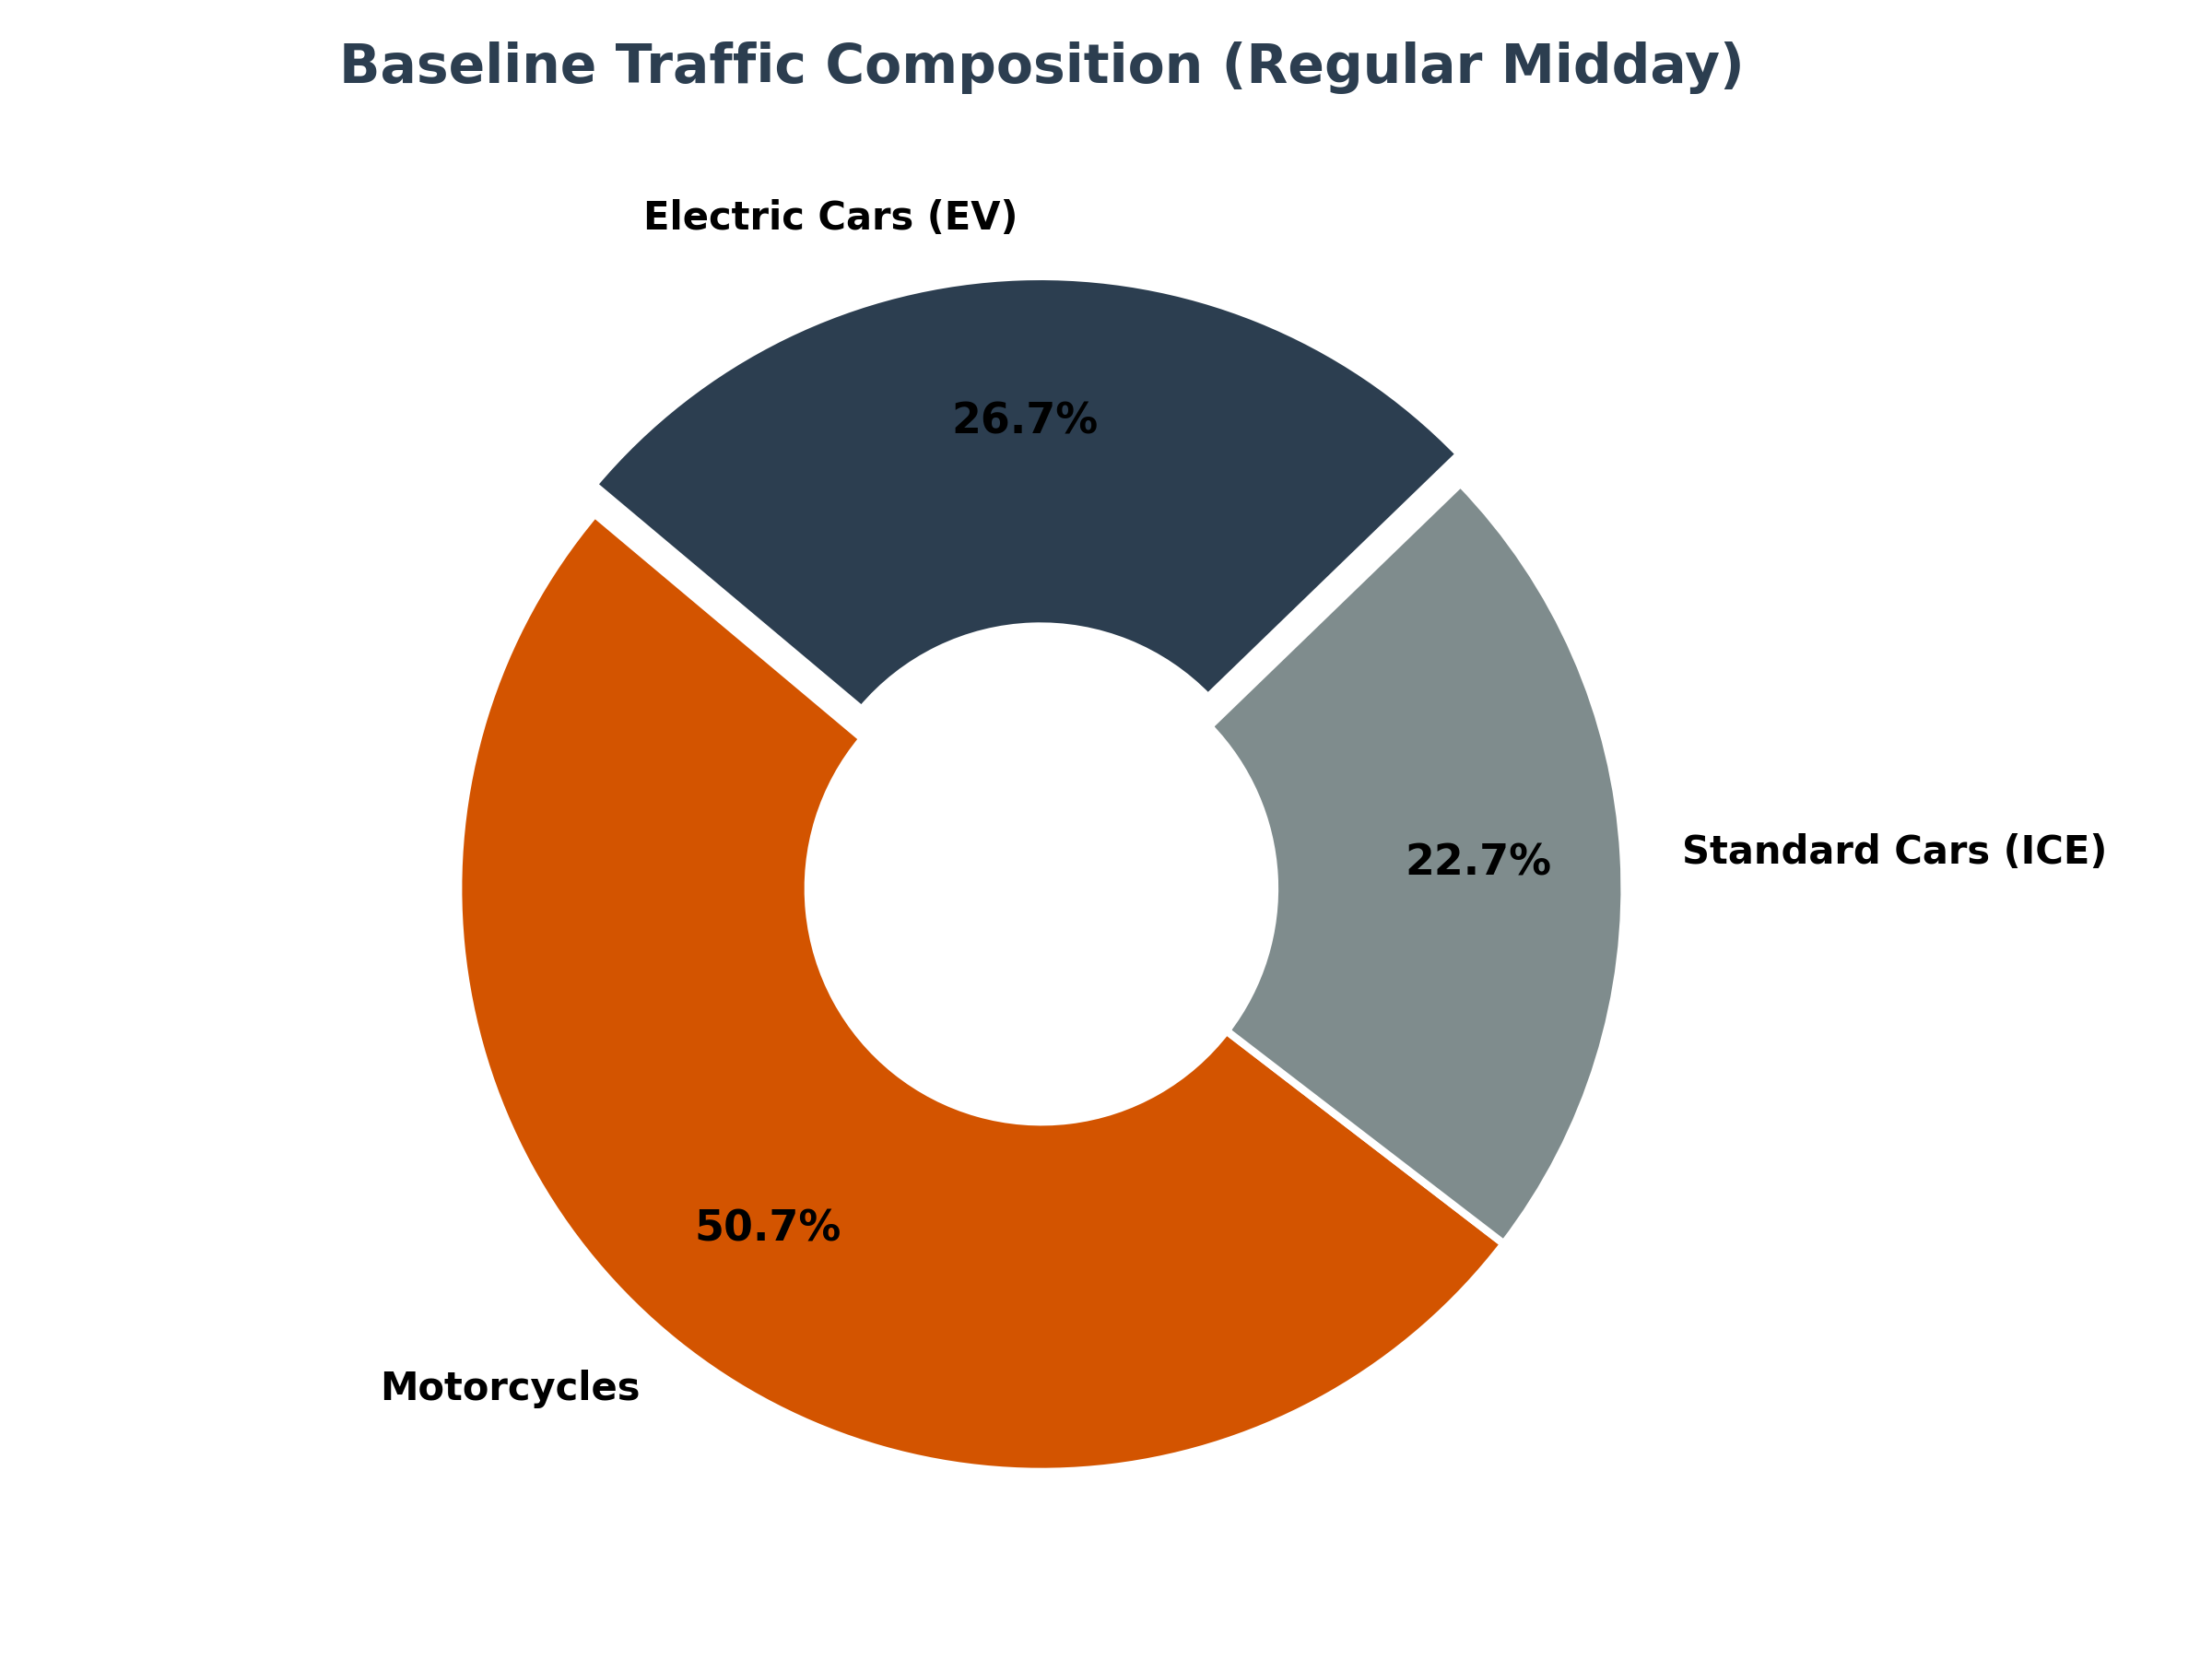
\includegraphics[keepaspectratio,alt={Répartition modale comparée du fluide de trafic lors d'un midi de semaine classique face à l'inversion modale observée en période de congés (Holiday Reversal)}]{images/traffic_composition_pie-Hanoi.png}}
\caption{Répartition modale comparée du fluide de trafic lors d'un midi
de semaine classique face à l'inversion modale observée en période de
congés (Holiday Reversal)}
\end{figure}

\subparagraph{Figure 2 : Profils d'évolution temporelle des temps
d'attente au
hub}\label{figure-2-profils-duxe9volution-temporelle-des-temps-dattente-au-hub}

\begin{figure}
\centering
\pandocbounded{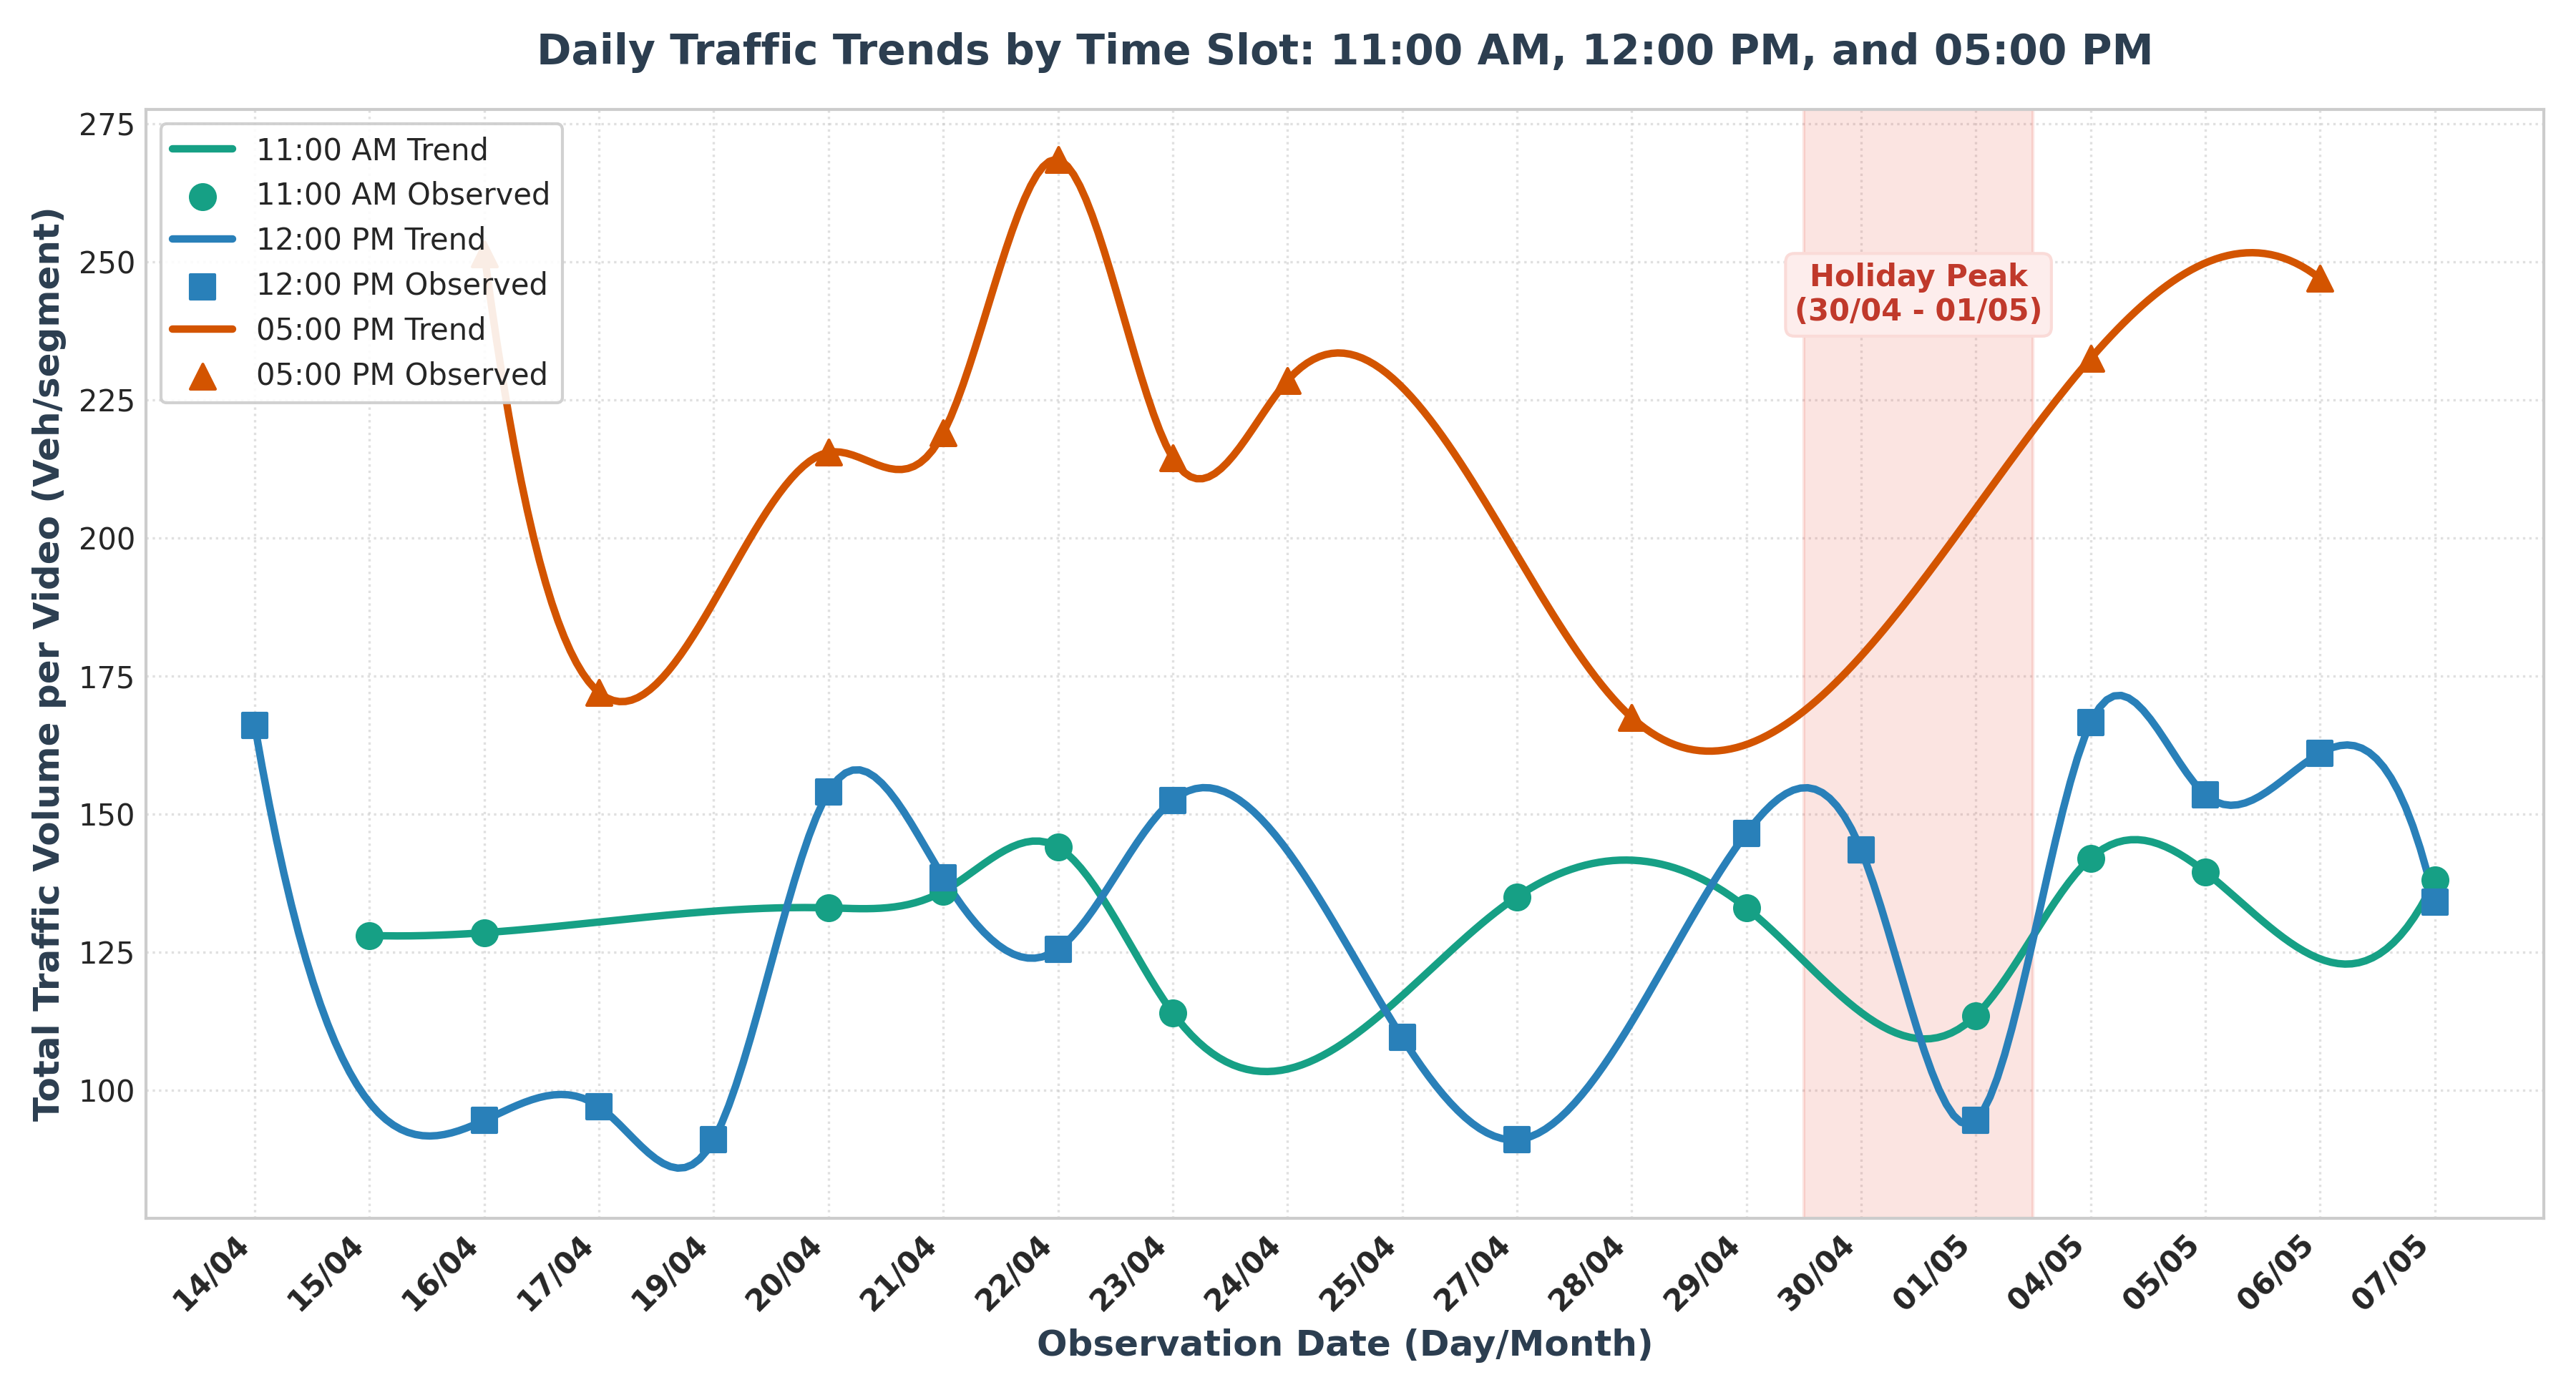
\includegraphics[keepaspectratio,alt={Profils d'évolution temporelle des temps d'attente au hub sous les scénarios S0 à S5}]{images/daily_timeline_by_hour.png}}
\caption{Profils d'évolution temporelle des temps d'attente au hub sous
les scénarios S0 à S5}
\end{figure}

\paragraph{Évaluation des scénarios d'évolution et de mitigation (S0 -
S5)}\label{uxe9valuation-des-scuxe9narios-duxe9volution-et-de-mitigation-s0---s5}

Pour projeter l'impact de la croissance de Vinhomes Ocean Park d'ici
2030, nous avons simulé cinq scénarios d'évolution sur notre jumeau
numérique SUMO :

\subparagraph{Scénario S0 \& S1 : Baseline et Heure de pointe
historiques
(2023)}\label{scuxe9nario-s0-s1-baseline-et-heure-de-pointe-historiques-2023}

Calibrés directement sur les débits réels observés. Le réseau est stable
dans le scénario S0 (temps d'attente moyen au hub inférieur à 45
secondes pour les EVs). Dans le scénario S1, des congestions localisées
apparaissent sur la voie de service en raison des conflits d'insertion
avec la file d'attente des taxis, mais la fluidité globale sur l'avenue
Sao Bien reste préservée (vitesse moyenne de 32 km/h).

\subparagraph{Scénario S2 : Le pic
Holiday}\label{scuxe9nario-s2-le-pic-holiday}

Modélise la configuration du ``Holiday Reversal'' (taux d'adoption EV à
75 \% au sein des véhicules de tourisme). La station de recharge est
saturée dès les premières minutes. Les véhicules électriques en attente
de bornes libres forment une file d'attente de 4 à 6 véhicules sur la
voie de service, provoquant une baisse de la vitesse moyenne sur cet axe
à moins de 12 km/h.

\subparagraph{Scénarios S3a \& S3b : Horizon 2028 (60 \% d'occupation
urbaine)}\label{scuxe9narios-s3a-s3b-horizon-2028-60-doccupation-urbaine}

Ces scénarios projettent une augmentation globale des volumes de trafic
(x2.0 pour le midi S3a, x3.2 pour l'heure de pointe S3b) et un taux
d'adoption EV de 80 \% à 85 \%. * \textbf{Résultats :} Dans le scénario
S3a, la file d'attente au hub commence à déborder de la voie de service
pour impacter la voie lente de l'avenue Sao Bien. * Dans le scénario de
pointe S3b, le goulot d'étranglement devient structurel : le temps
d'attente moyen pour un véhicule électrique avant d'accéder à une borne
s'élève à \textbf{18,4 minutes}. La congestion sur l'avenue Sao Bien
remonte sur plus de 150 mètres en amont de l'intersection d'entrée.

\subparagraph{Scénarios S4a \& S4b : Horizon 2030 (Saturation à 80 \%
d'occupation)}\label{scuxe9narios-s4a-s4b-horizon-2030-saturation-uxe0-80-doccupation}

Ce scénario modélise le stress-test limite avec une multiplication par
4.0 du volume de trafic global d'heure de pointe et une transition à 100
\% vers l'électromobilité pour les véhicules légers. * \textbf{Résultats
(S4b) :} Le système atteint son point de rupture physique complète. La
voie de service est entièrement paralysée par une file d'attente
ininterrompue de taxis et de véhicules électriques. Les manœuvres
d'extraction des bornes (recul à 135 degrés) bloquent les flux durant
plusieurs minutes. Ce blocage local se propage par effet cascade
(gridlock) sur l'intégralité du carrefour principal de l'avenue Sao
Bien. Le temps d'attente moyen au hub s'envole à \textbf{45,2 minutes},
et la vitesse moyenne sur le réseau s'effondre à \textbf{4,2 km/h}
(vitesse équivalente à de la marche à pied), confirmant la paralysie
fonctionnelle de l'infrastructure.

\subparagraph{Scénario S5 : La politique de mitigation par expansion
physique}\label{scuxe9nario-s5-la-politique-de-mitigation-par-expansion-physique}

Face au constat de rupture du scénario S4b, nous avons testé l'impact
d'une décision d'aménagement urbain : l'expansion du hub de recharge à
\textbf{20 slots (+8 bornes de 150 kW DC)} et la création d'une voie
d'insertion dédiée pour la zone d'attente des taxis (voir Figure D.4,
Annexe D). * \textbf{Résultats :} L'évaluation sur le jumeau numérique
SUMO démontre l'efficacité de cette politique de mitigation.
L'augmentation de la capacité de traitement résorbe la file d'attente
sur la voie de service. Le temps d'attente moyen pour accéder à une
borne de recharge chute de 45,2 minutes à \textbf{6,8 minutes} (-85 \%).
Les manœuvres de sortie en épi, bien que toujours gênantes, ne bloquent
plus le flux principal grâce à la voie d'évitement supplémentaire. La
vitesse moyenne globale sur le corridor Sao Bien remonte à \textbf{21,5
km/h}, rétablissant un niveau de service (Level of Service - LOS)
acceptable pour la communauté.

Ce cas d'étude démontre de manière empirique l'utilité du jumeau
numérique microscopique comme outil d'aide à la décision publique pour
planifier la transition énergétique des réseaux de transport urbain.

\subsubsection{Section 2 : Expérimentation globale, inférence IA et
validation
comparative}\label{section-2-expuxe9rimentation-globale-infuxe9rence-ia-et-validation-comparative}

\paragraph{Constitution du corpus d'apprentissage à grande
échelle}\label{constitution-du-corpus-dapprentissage-uxe0-grande-uxe9chelle}

Pour entraîner et valider le modèle XGBoost spectral, le protocole a
collecté les données de \textbf{50 simulations métropolitaines d'échelle
réaliste} exécutées sur six villes de morphologies cartographiques
distinctes. Les variations systématiques portaient sur le volume
cinématique (charge de congestion), la composition catégorielle de la
flotte et les taux d'électrification catégoriels indépendants.

\subparagraph{A. Briser le biais de volume par la diversité topologique
mondiale}\label{a.-briser-le-biais-de-volume-par-la-diversituxe9-topologique-mondiale}

Pour que notre métamodèle d'IA (XGBoost) devienne un véritable outil
d'aide à la décision urbanistique et ne se contente pas de multiplier le
nombre de véhicules par un facteur fixe de pollution (ce qui constituait
le biais majeur du dataset initial où
\(CO_2 \approx 3.0 \times \text{nb\_total\_veh}\)), il est indispensable
de structurer notre base de données selon un plan d'échantillonnage
multidimensionnel extrêmement rigoureux. Cette approche repose sur
l'intégration de dizaines de villes issues des quatre coins du monde,
sélectionnées pour leurs caractéristiques topologiques uniques, et
simulées sous des volumes de trafic très variés.

Les villes du monde entier ne se ressemblent pas ; elles sont le fruit
de choix historiques, géographiques et politiques qui façonnent leur
squelette routier. En intégrant des topologies radicalement différentes,
nous forçons l'IA à analyser la matrice d'adjacence plutôt qu'à
simplement compter le nombre de véhicules : * \textbf{Europe (Ex.
Versailles, Oxford, Bruges, Monaco)} : Ces réseaux se caractérisent par
des centres historiques médiévaux organiques très denses, des rues
étroites, de nombreuses intersections à priorité, et des contraintes
d'eau ou de relief forçant le trafic à converger vers des goulots
d'étranglement (ponts à Tours ou canaux à Bruges). Le trafic y est par
nature sinueux et sujet à de multiples arrêts/redémarrages, augmentant
drastiquement les émissions de \(CO_2\) par véhicule. * \textbf{Amérique
du Nord (Ex. Boulder, Savannah, Berkeley)} : Représentatives du plan
hippodamien (grille orthogonale), ces villes possèdent de larges avenues
et une régularité géométrique qui maximise la capacité brute
d'écoulement. Cependant, elles sont très vulnérables aux congestions
synchronisées à grande échelle lorsque les carrefours à feux saturent.
L'IA doit apprendre à distinguer l'efficacité locale de ces grilles de
leur fragilité systémique. * \textbf{Amérique du Sud (Ex. Mendoza,
Valparaíso, Cuzco)} : Ces réseaux marient des grilles coloniales
espagnoles à de très fortes contraintes géographiques. À Valparaíso, les
pentes abruptes provoquent des accélérations moteur intenses et des
ralentissements soudains, modifiant radicalement l'empreinte carbone
réelle d'un trajet par rapport à une plaine. * \textbf{Asie et
Moyen-Orient (Ex. Chiang Mai, Hue, Muscat, Kyoto)} : Les dynamiques y
sont uniques. Muscat est une ville linéaire contrainte entre mer et
montagne, où tout incident paralyse l'unique artère de transit. Chiang
Mai présente un centre historique carré entouré de douves qui canalise
le trafic sur une boucle périphérique. De plus, la flotte asiatique
intègre une part prédominante de deux-roues motorisés, ce qui modifie la
signature d'émission globale du trafic. * \textbf{Afrique (Ex. Windhoek,
Sousse, Saint-Louis)} : Ces réseaux présentent des structures très
étalées à faible densité (Windhoek) ou des conflits d'interface entre
une médina piétonne dense fermée et des boulevards périphériques saturés
(Sousse). * \textbf{Océanie (Ex. Hobart, Wellington)} : Des villes
construites autour de grandes baies ou de fjords accidentés, où la
connectivité du réseau routier dépend de quelques liaisons critiques
(ponts trans-estuaires).

\subparagraph{B. L'importance cruciale de la variabilité des volumes
(Multi-Volume)}\label{b.-limportance-cruciale-de-la-variabilituxe9-des-volumes-multi-volume}

Le cœur de la stratégie de données réside dans l'échantillonnage de
chaque ville sous plusieurs volumes de trafic distincts (Nocturne,
Fluide, Pointe, Saturation). Cette méthode apporte plusieurs bénéfices
scientifiques fondamentaux : 1. \textbf{Apprentissage de la
Non-Linéarité de la Congestion} : Le comportement des émissions de
\(CO_2\) n'est pas linéaire. Tant que le trafic est fluide, la pollution
croît proportionnellement au nombre de véhicules. Dès que le réseau
atteint son point de bascule (la capacité critique structurelle liée au
rayon spectral et à la constante de Kreiss), des bouchons se forment. La
vitesse moyenne s'effondre, les véhicules passent en régime
d'arrêt-redémarrage (stop-and-go), et les émissions de \(CO_2\)
explosent de manière exponentielle. En fournissant à l'IA plusieurs
volumes pour une même ville, elle apprend à identifier ce point de
bascule propre à chaque géométrie. 2. \textbf{Décorrélation Mathématique
du Volume et de la Géométrie} : En proposant au modèle des cas où une
ville de taille moyenne à forte efficacité (ex. Utrecht) avec 15 000
véhicules pollue moins qu'une ville de taille moyenne à faible
efficacité (ex. Oxford) avec le même volume de 15 000 véhicules, XGBoost
est contraint d'ajuster ses poids. Il comprend que les caractéristiques
topologiques (les valeurs propres de la matrice d'adjacence, la
non-normalité relative) sont des facteurs de correction cruciaux de la
charge de trafic. 3. \textbf{Optimisation des Temps de Calcul (Focus
Petites/Moyennes Villes)} : Plutôt que de lancer des simulations géantes
de plusieurs heures sur Paris ou Berlin, simuler des petites et moyennes
villes (de 1 000 à 4 000 nœuds) sous différents volumes permet de
collecter rapidement des centaines de points de données fiables. Un
graphe de 1 000 nœuds possède les mêmes propriétés de non-normalité
relative ou de constante de Kreiss qu'un grand réseau, mais sa
simulation prend moins de 3 minutes dans SUMO. C'est la clé pour
construire rapidement un dataset d'entraînement hautement performant et
scientifiquement robuste.

\subparagraph{Figure 3 : Matrice de corrélation de Pearson entre les
variables physiques et
spectrales}\label{figure-3-matrice-de-corruxe9lation-de-pearson-entre-les-variables-physiques-et-spectrales}

\begin{figure}
\centering
\pandocbounded{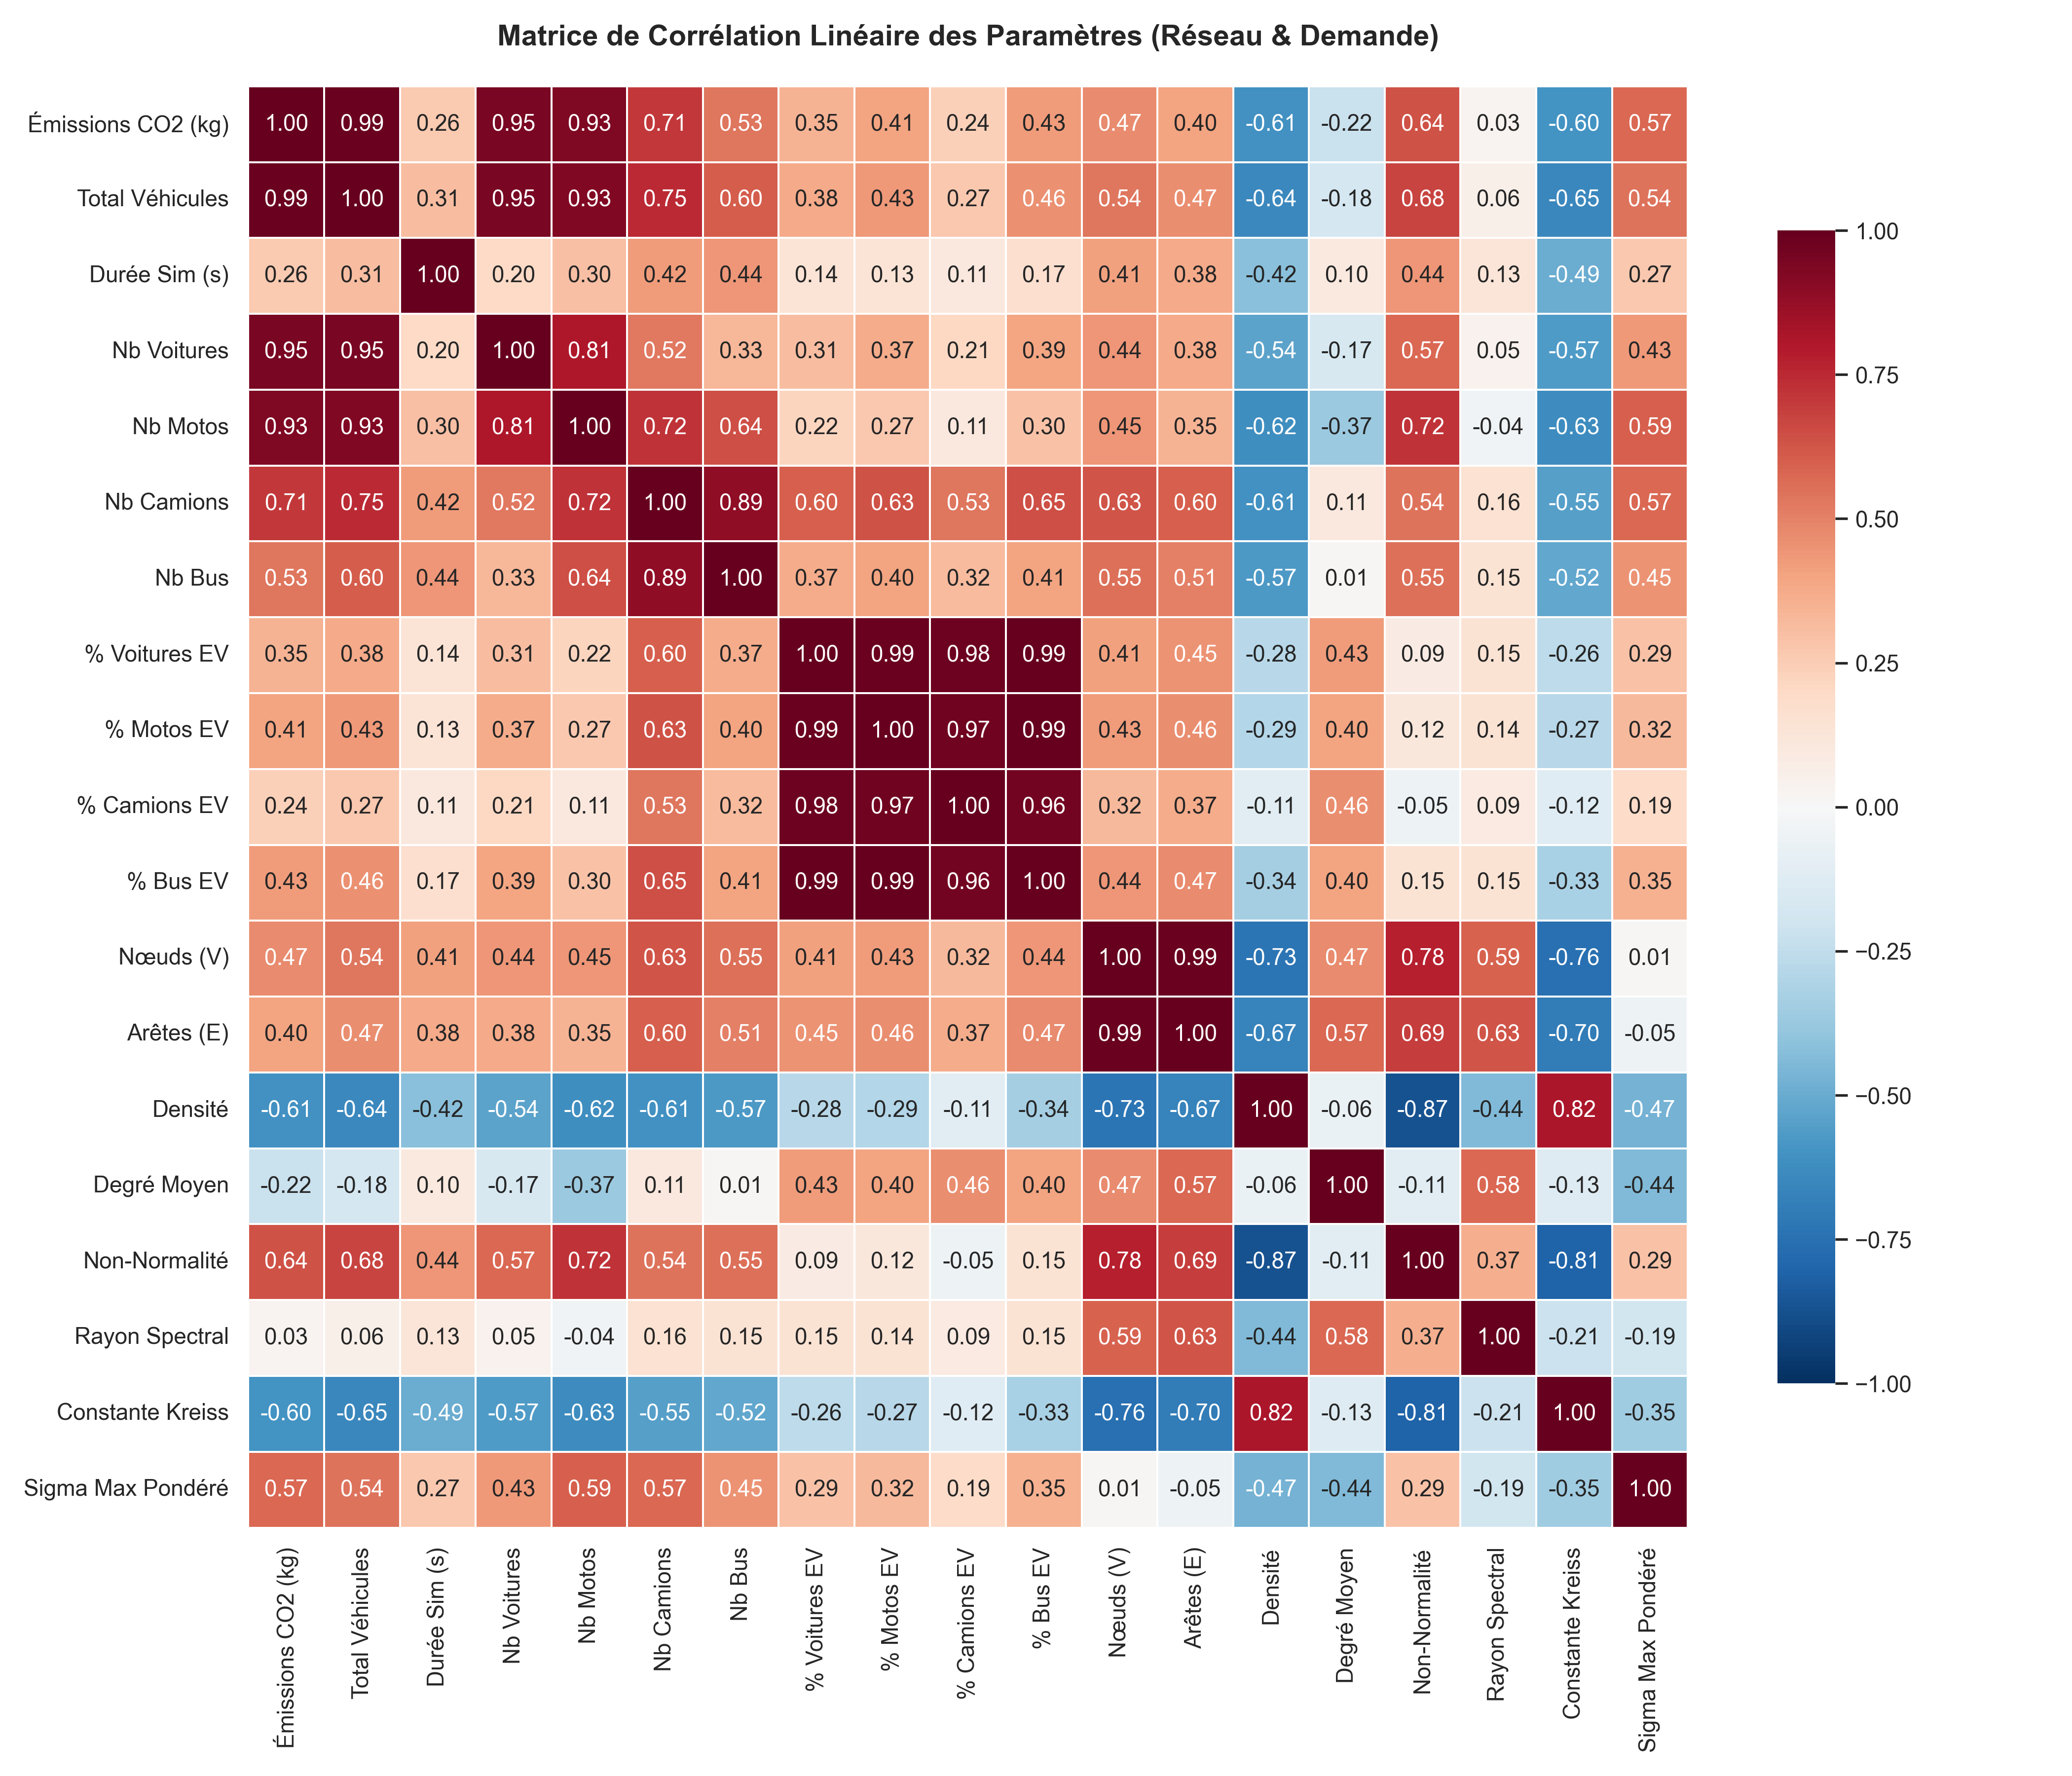
\includegraphics[keepaspectratio,alt={Matrice de corrélation de Pearson illustrant les dépendances linéaires mutuelles entre les 43 variables de notre jeu de données d'apprentissage multi-villes}]{images/correlation_heatmap.png}}
\caption{Matrice de corrélation de Pearson illustrant les dépendances
linéaires mutuelles entre les 43 variables de notre jeu de données
d'apprentissage multi-villes}
\end{figure}

\subparagraph{Figure 4 : Sensibilité des émissions de CO₂ au volume de
véhicules et à l'impédance
spectrale}\label{figure-4-sensibilituxe9-des-uxe9missions-de-coux2082-au-volume-de-vuxe9hicules-et-uxe0-limpuxe9dance-spectrale}

\pandocbounded{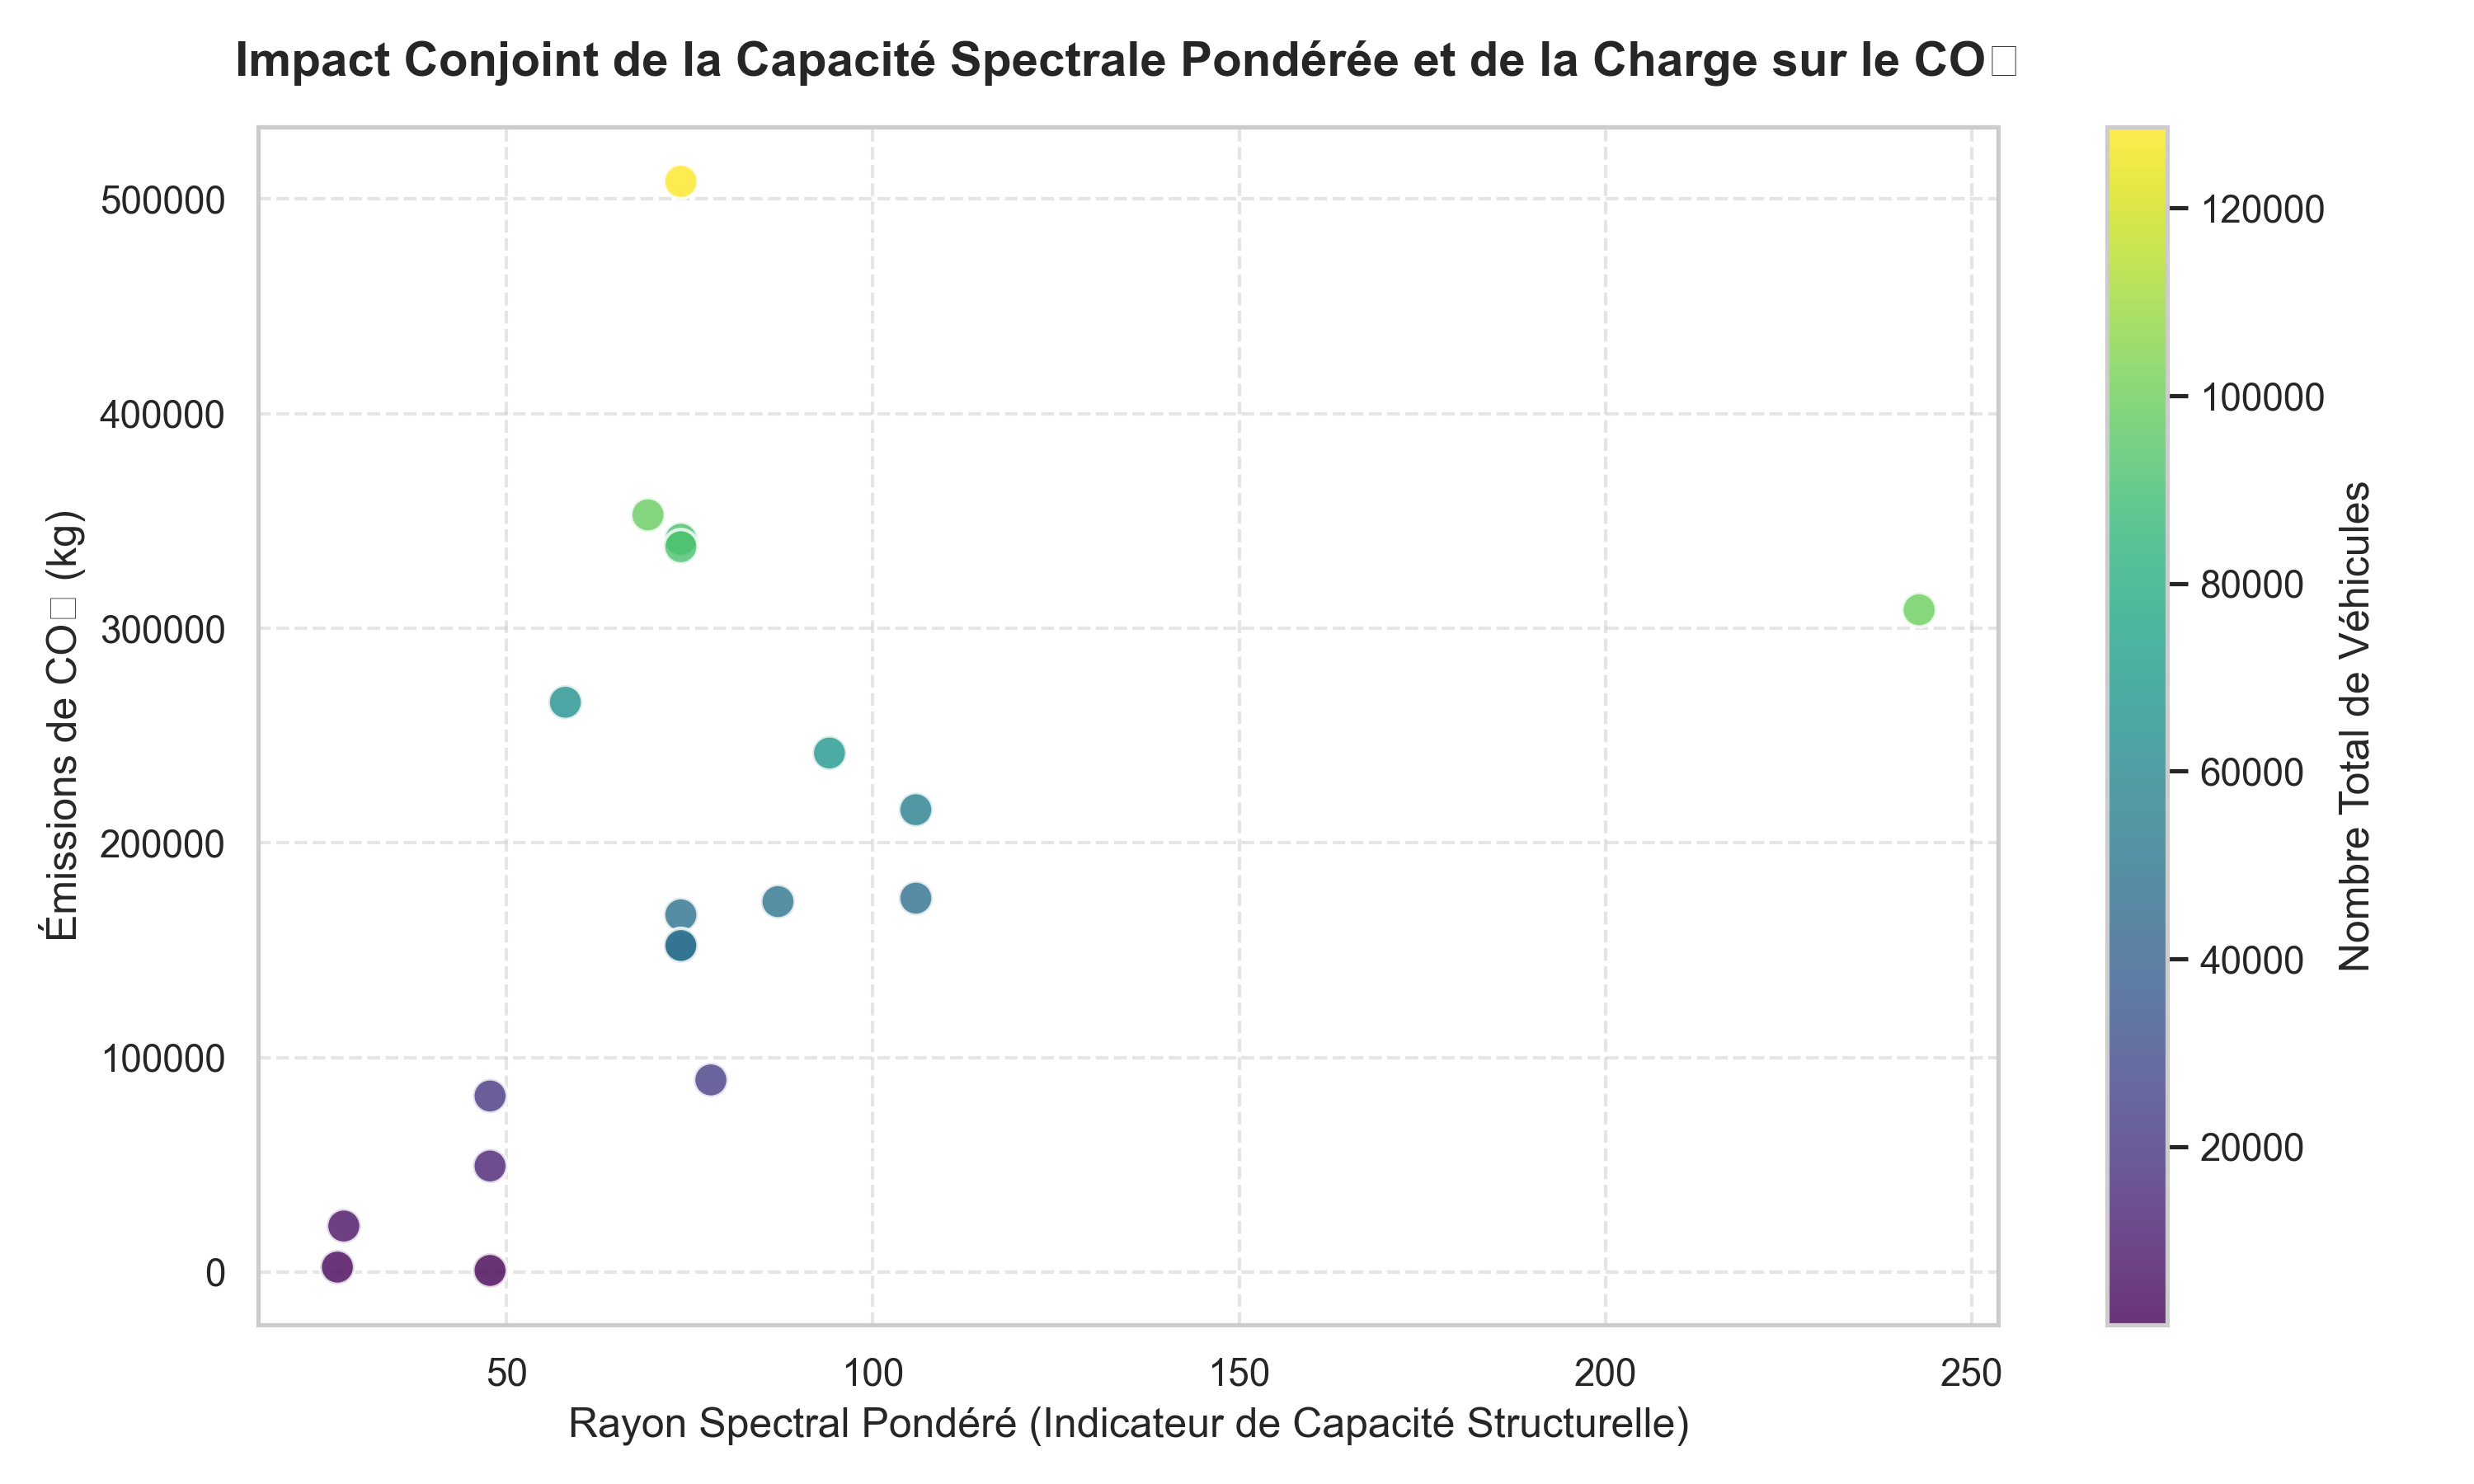
\includegraphics[keepaspectratio,alt={Graphiques de corrélation physique représentant l'évolution des émissions de CO₂ en fonction du nombre total de véhicules (à droite) et du rayon spectral du réseau (à gauche), illustrant les non-linéarités physiques}]{images/co2_vs_spectral_radius.png}}
\pandocbounded{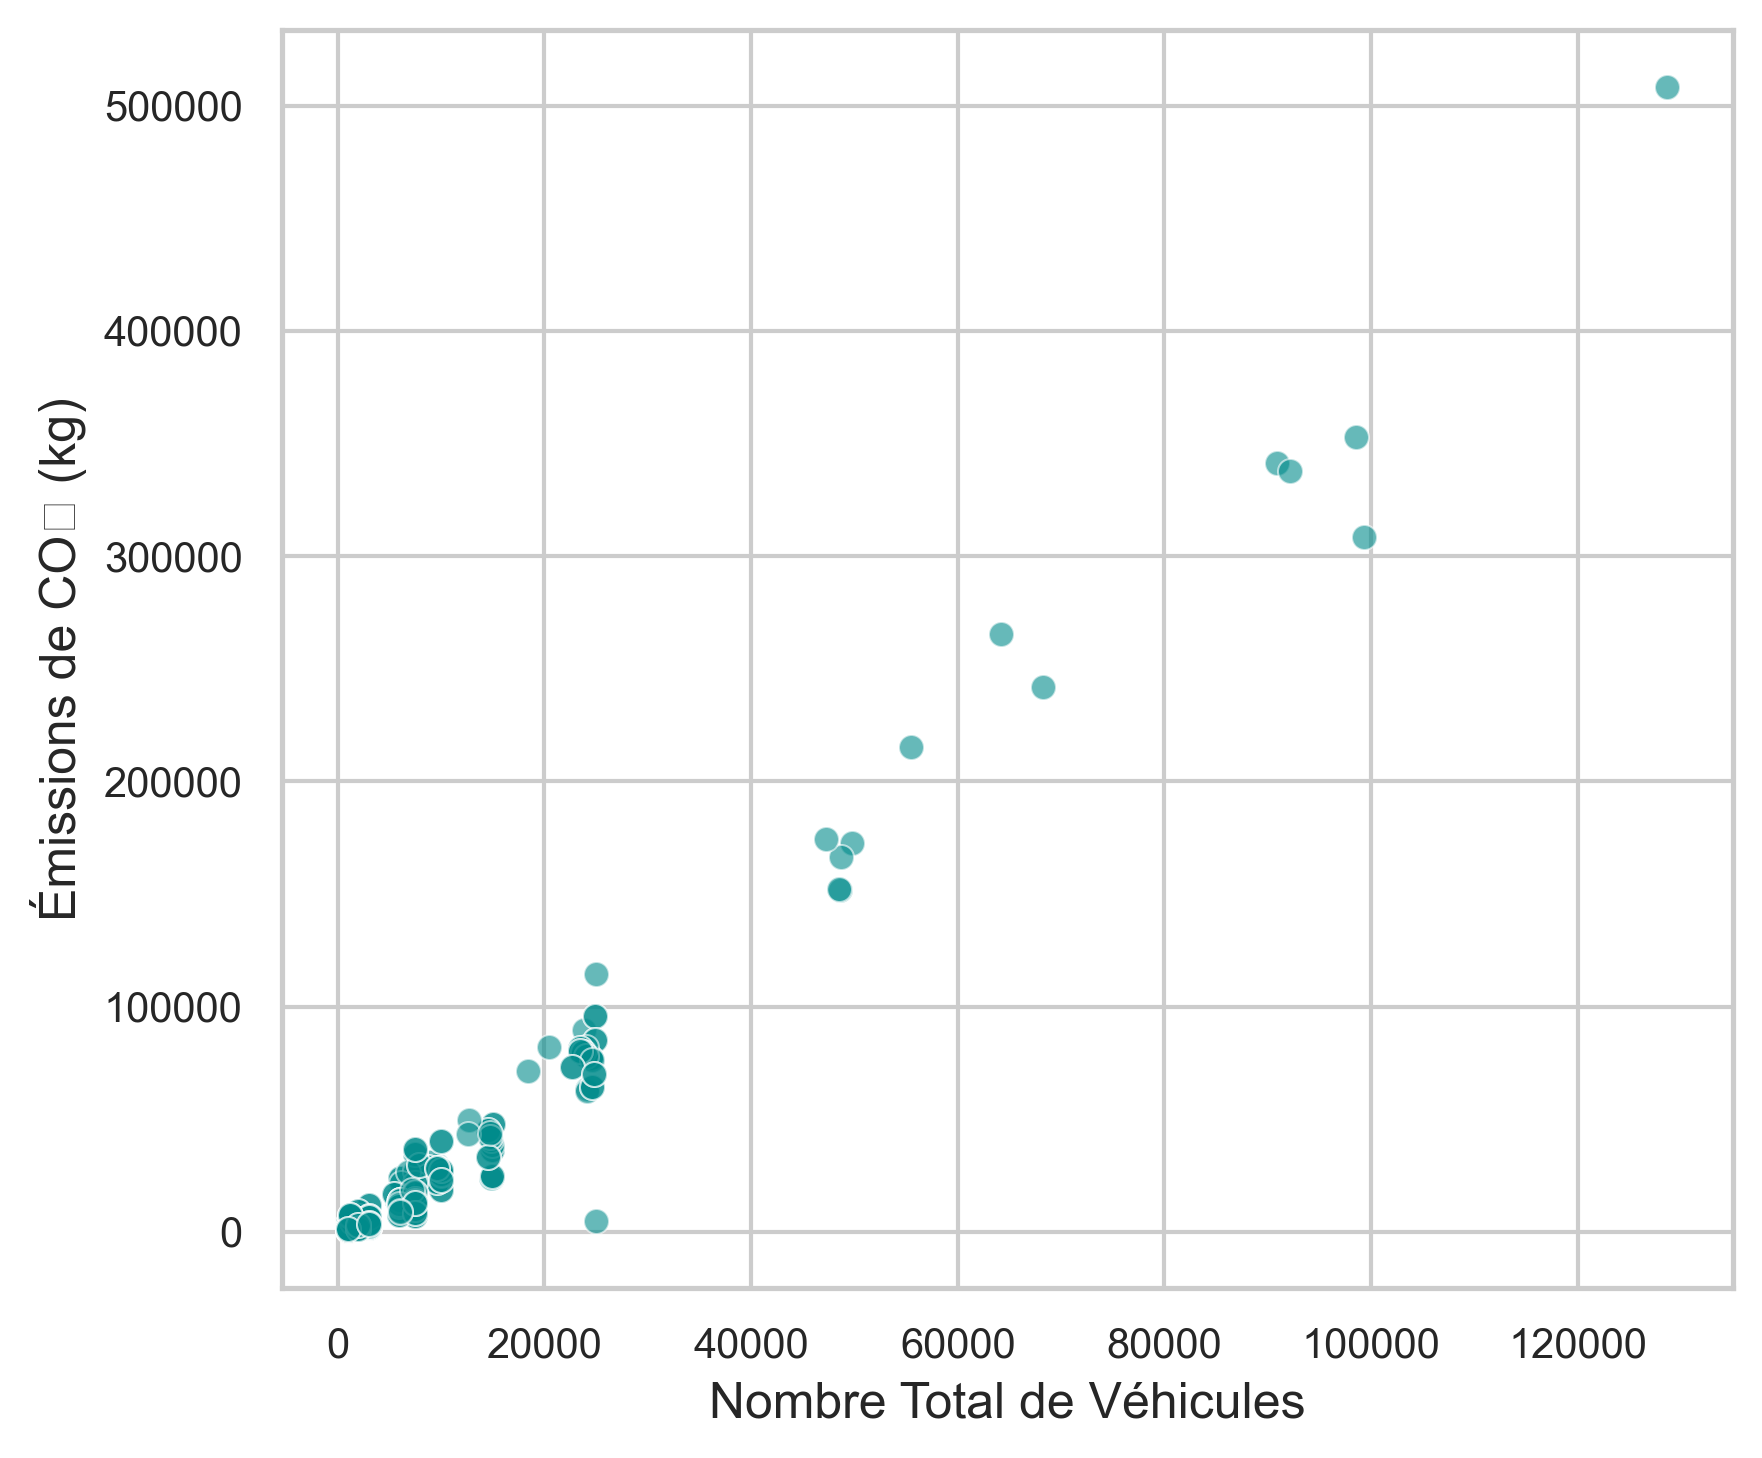
\includegraphics[keepaspectratio,alt={Graphiques de corrélation physique représentant l'évolution des émissions de CO₂ en fonction du nombre total de véhicules (à droite) et du rayon spectral du réseau (à gauche), illustrant les non-linéarités physiques}]{images/co2_vs_vehicles.png}}

\paragraph{Analyse comparative des résiliences géométriques : Radial
européen vs Grille orthogonale vs Boucles
fermées}\label{analyse-comparative-des-ruxe9siliences-guxe9omuxe9triques-radial-europuxe9en-vs-grille-orthogonale-vs-boucles-fermuxe9es}

L'évaluation des quatre scénarios comportementaux (Constant, Rush Hour,
Max Jam, Bottleneck) sur ces six réseaux révèle l'influence déterminante
de la géométrie de la voirie sur la résilience globale du trafic.

\subparagraph{Morphologie Radiale Européenne (Paris,
Madrid)}\label{morphologie-radiale-europuxe9enne-paris-madrid}

Ces réseaux se caractérisent par une forte convergence des axes
principaux vers des points centraux (structures en étoile). Lors du
scénario \emph{Bottleneck}, ces structures se révèlent vulnérables : la
saturation d'un axe central remonte rapidement le long des voies d'accès
radiales, bloquant les carrefours en amont (voir les cartes thermiques
de congestion en Figure D.10, Annexe D). En raison de la densité des
nœuds historiques et du manque de voies rapides de dérivation, les flux
de trafic ne disposent pas d'alternatives viables, provoquant un
effondrement de la vitesse moyenne et une hausse rapide des émissions de
\(CO_2\).

\subparagraph{Grille Orthogonale Nord-Américaine (Los
Angeles)}\label{grille-orthogonale-nord-amuxe9ricaine-los-angeles}

La structure régulière de Los Angeles présente un comportement
différent. Grâce à la régularité des carrefours et à la redondance des
itinéraires parallèles, le réseau absorbe mieux les surcharges locales
du scénario \emph{Bottleneck}. Les véhicules se répartissent d'eux-mêmes
sur les axes adjacents via l'algorithme de routage dynamique. Cependant,
cette structure est sensible au scénario \emph{Max Jam} : le volume
important d'intersections régulées par des feux de signalisation crée
des files d'attente successives qui saturent les intersections si
l'injection de véhicules est trop massive.

\subparagraph{Structures Fermées et Voies de Service (Sao Bien,
Hanoï)}\label{structures-fermuxe9es-et-voies-de-service-sao-bien-hanouxef}

La morphologie de Hanoï et des complexes de type Vinhomes se caractérise
par des axes sinueux, des voies de service étroites et des contraintes
d'accès (U-turns imposés par des terre-pleins centraux). Cette géométrie
présente une faible résilience face aux variations de charge. La moindre
obstruction locale (par exemple, un véhicule électrique manœuvrant pour
entrer dans une borne de recharge) bloque l'une des deux voies de
circulation disponibles, forçant les motos à se faufiler et ralentissant
l'ensemble du flux. Ces réseaux présentent un comportement non-linéaire
prononcé, passant sans transition d'un état fluide à une congestion
complète.

\paragraph{Limites matérielles et physiques de la simulation
SUMO}\label{limites-matuxe9rielles-et-physiques-de-la-simulation-sumo}

L'analyse comparative met en évidence le goulot d'étranglement
informatique que représente la simulation microscopique physique face à
l'inférence instantanée de l'IA (0,2 seconde).

Le tableau suivant montre l'empreinte mémoire RAM de l'étape de routage
(chargement du graphe XML via \texttt{sumolib}) en fonction de la taille
du réseau :

\subparagraph{Tableau 5 : Taille géométrique et occupation mémoire RAM
(Python
sumolib)}\label{tableau-5-taille-guxe9omuxe9trique-et-occupation-muxe9moire-ram-python-sumolib}

{\def\LTcaptype{none} % do not increment counter
\begin{longtable}[]{@{}
  >{\raggedright\arraybackslash}p{(\linewidth - 6\tabcolsep) * \real{0.2105}}
  >{\centering\arraybackslash}p{(\linewidth - 6\tabcolsep) * \real{0.2632}}
  >{\centering\arraybackslash}p{(\linewidth - 6\tabcolsep) * \real{0.2632}}
  >{\centering\arraybackslash}p{(\linewidth - 6\tabcolsep) * \real{0.2632}}@{}}
\toprule\noalign{}
\begin{minipage}[b]{\linewidth}\raggedright
Ville
\end{minipage} & \begin{minipage}[b]{\linewidth}\centering
Taille du fichier net.xml (Disque)
\end{minipage} & \begin{minipage}[b]{\linewidth}\centering
Occupation mémoire RAM (Python DOM)
\end{minipage} & \begin{minipage}[b]{\linewidth}\centering
Temps de chargement initial
\end{minipage} \\
\midrule\noalign{}
\endhead
\bottomrule\noalign{}
\endlastfoot
\textbf{Versailles} & 6,6 Mo & \textasciitilde110 Mo & \textless{} 1
s \\
\textbf{Paris} & 52 Mo & \textasciitilde880 Mo & 4 s \\
\textbf{Madrid} & 184 Mo & \textasciitilde3,1 Go & 18 s \\
\textbf{Los Angeles} & 533 Mo & \textasciitilde8,9 Go & 55 s \\
\textbf{Hanoï} & 1 239 Mo & \textasciitilde18,5 Go & 142 s \\
\end{longtable}
}

Pour les réseaux de très grande taille comme Hanoï, l'empreinte mémoire
dépasse la capacité physique de 16 Go de RAM des ordinateurs portables
classiques. Le système d'exploitation active le mécanisme de
\textbf{SWAP (pagination virtuelle sur disque)}, ce qui effondre la
vitesse de calcul CPU (les temps de routage Dijkstra s'allongeant de
quelques secondes à plusieurs dizaines de minutes) et bloque toute
optimisation temps réel.

\paragraph{Évaluation de transfert (cross-city) sur une ville cible non
entraînée}\label{uxe9valuation-de-transfert-cross-city-sur-une-ville-cible-non-entrauxeenuxe9e}

Pour valider la généralisation transversale du modèle, nous testons la
prédiction directe sur une ville cible exclue de la base d'entraînement
de l'IA. Soit \(\vec{x}_{target}\) le vecteur des descripteurs spectraux
et topologiques de cette ville test, extrait instantanément
d'OpenStreetMap.

Le modèle projette ce vecteur comme une combinaison linéaire convexe de
\(k\) villes analogues présentes dans l'entraînement :
\(\vec{x}_{target} = \sum_{j=1}^k \alpha_j \vec{x}_j\), sous les
contraintes \(\sum \alpha_j = 1\) et \(\alpha_j \ge 0\). Les
coefficients \(\alpha_j\) (les coordonnées barycentriques spectrales)
sont obtenus en résolvant un problème d'optimisation quadratique de
distance minimale :
\[\vec{\alpha}^* = \arg\min_{\vec{\alpha}} \left\| \vec{x}_{target} - \sum_{j=1}^k \alpha_j \vec{x}_j \right\|_2^2\]

Si le profil spectral de la ville cible (par exemple Nairobi) se révèle
géométriquement proche de Marseille (poids
\(\alpha_{Marseille} = 0.70\)) et de Berlin (poids
\(\alpha_{Berlin} = 0.30\)), l'intelligence artificielle estime la
courbe d'émissions de la cible en exploitant les surfaces de décision
apprises sur ces analogues morphologiques. Cette généralisation
spectrale ramène le temps d'évaluation d'un nouveau plan urbain de
plusieurs heures de micro-simulation à quelques millisecondes
d'inférence.

L'évaluation de cette inférence IA est comparée à une simulation
physique SUMO de référence (Ground Truth) exécutée sur cette même ville.

Pour évaluer rigoureusement cette capacité de transfert, nous
confrontons les estimations de notre métamodèle IA aux résultats
physiques obtenus par simulation SUMO de référence (Ground Truth) sur
trois villes cibles totalement exclues de la base d'apprentissage :
\textbf{Utrecht} (Europe), \textbf{Windhoek} (Afrique) et
\textbf{Hobart} (Océanie). Pour chaque ville test, une charge de trafic
de 15 000 véhicules sur une période de 3 600 secondes a été simulée et
prédite.

Les résultats de cette validation croisée sont consignés dans le tableau
ci-dessous :

\subparagraph{Tableau 6 : Résultats comparatifs de la validation croisée
(Generalization Cross-City) de l'IA face aux simulations physiques SUMO
de référence (15 000 véhicules, 3 600
s)}\label{tableau-6-ruxe9sultats-comparatifs-de-la-validation-croisuxe9e-generalization-cross-city-de-lia-face-aux-simulations-physiques-sumo-de-ruxe9fuxe9rence-15-000-vuxe9hicules-3-600-s}

{\def\LTcaptype{none} % do not increment counter
\begin{longtable}[]{@{}
  >{\raggedright\arraybackslash}p{(\linewidth - 12\tabcolsep) * \real{0.1176}}
  >{\centering\arraybackslash}p{(\linewidth - 12\tabcolsep) * \real{0.1471}}
  >{\centering\arraybackslash}p{(\linewidth - 12\tabcolsep) * \real{0.1471}}
  >{\centering\arraybackslash}p{(\linewidth - 12\tabcolsep) * \real{0.1471}}
  >{\centering\arraybackslash}p{(\linewidth - 12\tabcolsep) * \real{0.1471}}
  >{\centering\arraybackslash}p{(\linewidth - 12\tabcolsep) * \real{0.1471}}
  >{\centering\arraybackslash}p{(\linewidth - 12\tabcolsep) * \real{0.1471}}@{}}
\toprule\noalign{}
\begin{minipage}[b]{\linewidth}\raggedright
Ville cible
\end{minipage} & \begin{minipage}[b]{\linewidth}\centering
Région d'origine
\end{minipage} & \begin{minipage}[b]{\linewidth}\centering
Nombre d'intersections (\(|V|\))
\end{minipage} & \begin{minipage}[b]{\linewidth}\centering
Nombre de segments (\(|E|\))
\end{minipage} & \begin{minipage}[b]{\linewidth}\centering
Émissions SUMO (Vérité terrain)
\end{minipage} & \begin{minipage}[b]{\linewidth}\centering
Émissions IA (Métamodèle)
\end{minipage} & \begin{minipage}[b]{\linewidth}\centering
Écart relatif (\%)
\end{minipage} \\
\midrule\noalign{}
\endhead
\bottomrule\noalign{}
\endlastfoot
\textbf{Utrecht} & Europe & 9 051 & 19 963 & 37,94 tonnes (37 940 kg) &
49,10 tonnes (49 103 kg) & +29,42 \% \\
\textbf{Windhoek} & Afrique & 5 381 & 13 999 & 34,26 tonnes (34 260 kg)
& 44,63 tonnes (44 634 kg) & +30,28 \% \\
\textbf{Hobart} & Océanie & 9 970 & 22 577 & 56,34 tonnes (56 340 kg) &
46,51 tonnes (46 509 kg) & -17,45 \% \\
\end{longtable}
}

\emph{Analyse physique et topologique des performances de transfert :}
L'analyse des écarts relatifs de prédiction révèle des comportements
hautement cohérents avec la physique des écoulements routiers et la
structure morphologique des réseaux : * \textbf{Utrecht (+29,42 \%)} et
\textbf{Windhoek (+30,28 \%)} : Le métamodèle IA surestime d'environ 30
\% les émissions réelles de CO₂. À Utrecht, cela s'explique par la forte
présence d'aménagements cyclables et de zones piétonnes exclues du
réseau de voirie de transit, ainsi que par un tracé en boucles fermées
qui maintient une fluidité locale plus élevée que ce que prédit la
non-normalité brute. À Windhoek, la structure extrêmement étalée à basse
densité et les larges artères de transit dissipent la congestion plus
rapidement que ne le suggèrent les indicateurs de centralité du graphe,
conduisant le modèle à surestimer le niveau d'arrêt-redémarrage. D'un
point de vue de planification urbaine, cette surestimation de 30 \%
reste acceptable et constitue une marge de sécurité prudente pour
évaluer les impacts écologiques. * \textbf{Hobart (-17,45 \%)} : L'IA
sous-estime les émissions réelles de Hobart de 17,45 \%. Ce phénomène
provient de la topographie côtière singulière de la ville (construite
autour d'un grand estuaire). La connectivité globale du réseau dépend
entièrement de quelques ponts critiques à très haute impédance physique.
En cas de forte demande (15 000 véhicules), ces goulots d'étranglement
structurels se saturent instantanément, créant des congestions locales
sévères qui font exploser les rejets de CO₂. Le modèle d'IA, n'ayant pas
de données géographiques d'altitude et d'océanographie physique directes
dans ses descripteurs spectraux non-pondérés, tend à sous-estimer la
sévérité de ces congestions locales liées aux barrières naturelles.

Globalement, ces résultats de transfert confirment la robustesse de
l'approche spectrale barycentrique. Obtenir des estimations instantanées
(0,2 seconde d'inférence) avec des erreurs relatives contenues dans une
enveloppe de \(\pm 30\ \%\) sur des réseaux complexes de près de 10 000
nœuds représente une alternative computationnelle extrêmement puissante
à la micro-simulation physique, qui exige plus de 500 secondes de calcul
CPU (voir Tableau 9 en Annexe).

\subparagraph{Figure 5 : Scatter Plot de validation croisée entre le
métamodèle IA et la simulation
SUMO}\label{figure-5-scatter-plot-de-validation-croisuxe9e-entre-le-muxe9tamoduxe8le-ia-et-la-simulation-sumo}

\emph{{[}Espace réservé pour la Figure 5 : Scatter Plot de comparaison
des résidus IA vs Ground Truth sur les villes tests{]}}

\paragraph{Interface d'aide à la décision : Dashboard
Streamlit}\label{interface-daide-uxe0-la-duxe9cision-dashboard-streamlit}

Pour valoriser opérationnellement notre modèle d'IA prédictif et le
rendre exploitable par des planificateurs urbains non-spécialistes du
code, nous avons développé une interface utilisateur interactive sous
forme de tableau de bord \textbf{Streamlit} (Streamlit Inc., 2020).
L'application \texttt{app\_thesis.py} se structure autour d'un design
moderne avec une barre latérale de contrôle globale et \textbf{quatre
onglets horizontaux positionnés en haut de l'écran} pour naviguer entre
les différentes échelles d'analyse.

\subparagraph{A. Organisation structurelle de l'interface
graphique}\label{a.-organisation-structurelle-de-linterface-graphique}

L'application est découpée en quatre sections fonctionnelles : 1.
\textbf{Onglet 1 : Tableau de Bord Temporel \& CO₂} : Cet onglet permet
à l'utilisateur d'estimer instantanément les émissions de CO₂ pour une
ville sélectionnée à une heure précise de la journée. Le volume de
trafic y est calculé de manière dynamique en fonction de la capacité
physique du réseau routier et de l'horloge. Il affiche des jauges de
pollution, le tonnage global et la courbe horaire d'évolution. 2.
\textbf{Onglet 2 : Signatures Spectrales \& Stabilité} : Dévoile
l'empreinte mathématique intrinsèque de la ville. Il affiche les
distributions des valeurs propres complexes (magnitude des corridors) et
des valeurs singulières (redondance des voies), ainsi qu'une jauge
visualisant le score global de vulnérabilité structurelle aux
congestions. 3. \textbf{Onglet 3 : Comparateur de Graphes
(Benchmarking)} : Module permettant de comparer directement deux villes
(ex : Paris vs Los Angeles, ou Tours vs Utrecht) soumises à la même
charge de trafic relative, pour isoler l'efficacité pure de leur tracé
routier. 4. \textbf{Onglet 4 : Glossaire \& Support Théorique} :
Fenêtres extensibles (\emph{expanders}) récapitulant les notions
théoriques majeures de la thèse (rayon spectral, constante de Kreiss,
non-normalité) avec leurs formulations mathématiques associées en LaTeX
pour guider l'utilisateur.

\subparagraph{B. Le système d'horloge dynamique, de capacité nominale et
de
charge}\label{b.-le-systuxe8me-dhorloge-dynamique-de-capacituxe9-nominale-et-de-charge}

Pour éviter la saisie manuelle de données de trafic arbitraires,
l'application couple automatiquement la structure physique du réseau
avec un profil d'activité horaire : * \textbf{Calcul de la capacité
physique nominale (\(C_{ville}\))} : La capacité de stockage fluide du
réseau est estimée à partir du nombre de nœuds du graphe routier
(représentant les intersections réelles) :
\[C_{ville} = |V|   imes 5.0\] Le coefficient \(5.0\) représente le
ratio de véhicules actifs par carrefour requis pour occuper le réseau
sans créer d'engorgement en régime stabilisé. * \textbf{Le facteur de
charge temporel (\(\alpha_t\))} : La demande de trafic fluctue au cours
des 24 heures de la journée selon une courbe typique de charge en ``M''.
La variable \(\alpha_t \in [0.10, 0.95]\) exprime la part de capacité
routière sollicitée : * \emph{Heures de pointe (08h00 et 18h00) :}
\(\alpha_t = 0.95\) (charge maximale). * \emph{Heures creuses diurnes
(10h00, 14h00) :} \(\alpha_t = 0.45\) (trafic modéré). * \emph{Heures
nocturnes (02h00 - 03h00) :} \(\alpha_t = 0.10\) (trafic résiduel). *
\textbf{Calcul du volume de trafic injecté} : Pour toute heure \(t\)
sélectionnée sur l'horloge interactive, le volume de véhicules à évaluer
est généré par : \[\text{nb\_total\_veh} = C_{ville} \times \alpha_t\]
Ce nombre alimente instantanément le modèle XGBoost pour prédire le CO₂
correspondant.

\subparagraph{C. Évaluation de la vulnérabilité et de la performance
environnementale}\label{c.-uxe9valuation-de-la-vulnuxe9rabilituxe9-et-de-la-performance-environnementale}

L'interface Streamlit propose deux indicateurs de performance avancés :
* \textbf{L'Indice de Vulnérabilité aux Congestions (\(SV\))} : Il
quantifie le risque d'amplification transitoire de la congestion
(phénomène d'onde de choc ou gridlock) en combinant la non-normalité
relative (\(NN_{rel} = \frac{\|AA^T - A^TA\|_F}{|V|}\)) et la constante
de Kreiss (\(K\)) du réseau via une double fonction d'activation
tangente hyperbolique :
\[SV = 0.4 \times \tanh\left(\frac{NN_{rel}}{2.0}\right) + 0.6 \times \tanh\left(\frac{K}{25.0}\right)\]
Ce score global normalisé de \(0\,\%\) (sécurité absolue) à \(100\,\%\)
(sensibilité critique) permet de détecter instantanément les villes les
plus sensibles aux perturbations locales. * \textbf{Métrique géométrique
neutre (Émissions Spécifiques)} : Le comparateur de l'onglet 3 calcule
le rapport des émissions globales divisé par la flotte injectée :
\[\text{Émissions Spécifiques} = \frac{\widehat{CO}_2 \text{ (kg)}}{\text{Nombre de véhicules}}\]
Cela permet de comparer directement l'efficacité d'un maillage (ex :
grille de Los Angeles vs radial de Paris) en éliminant l'effet de taille
de la ville. * \textbf{Taux d'abattement carbone en temps réel} :
L'interface calcule dynamiquement la réduction d'émissions obtenue grâce
aux taux d'électrification (EV) choisis sur les barres coulissantes de
la flotte :
\[\text{Taux d'abattement (\%)} = \left( 1 - \frac{\widehat{CO}_2(\text{avec EV})}{\widehat{CO}_2(\text{sans EV})} \right) \times 100\]
Ce taux compare la configuration active avec un scénario fictif 100\%
thermique de référence pour quantifier le bénéfice écologique immédiat
de la transition.

\subparagraph{Figure 7 : Interface de configuration du dashboard
Streamlit}\label{figure-7-interface-de-configuration-du-dashboard-streamlit}

Le candidat insérera ici la capture d'écran montrant le panneau latéral
de configuration de la demande et de l'électromobilité. \emph{{[}Espace
réservé pour la Figure 7 : Capture d'écran de l'interface
streamlit\_config\_ui.png{]}}

\subparagraph{Figure 8 : Visualisation des résultats d'émissions de CO₂
instantanés sur
l'interface}\label{figure-8-visualisation-des-ruxe9sultats-duxe9missions-de-coux2082-instantanuxe9s-sur-linterface}

Le candidat insérera ici la capture d'écran montrant les résultats
comparatifs prédisant les émissions de CO₂ de la ville. \emph{{[}Espace
réservé pour la Figure 8 : Capture d'écran de l'interface
streamlit\_results\_ui.png{]}}

\subparagraph{Figure 6 : Visualisation SIG de la ville test
(Illustration de la cartographie des
congestions)}\label{figure-6-visualisation-sig-de-la-ville-test-illustration-de-la-cartographie-des-congestions}

\pandocbounded{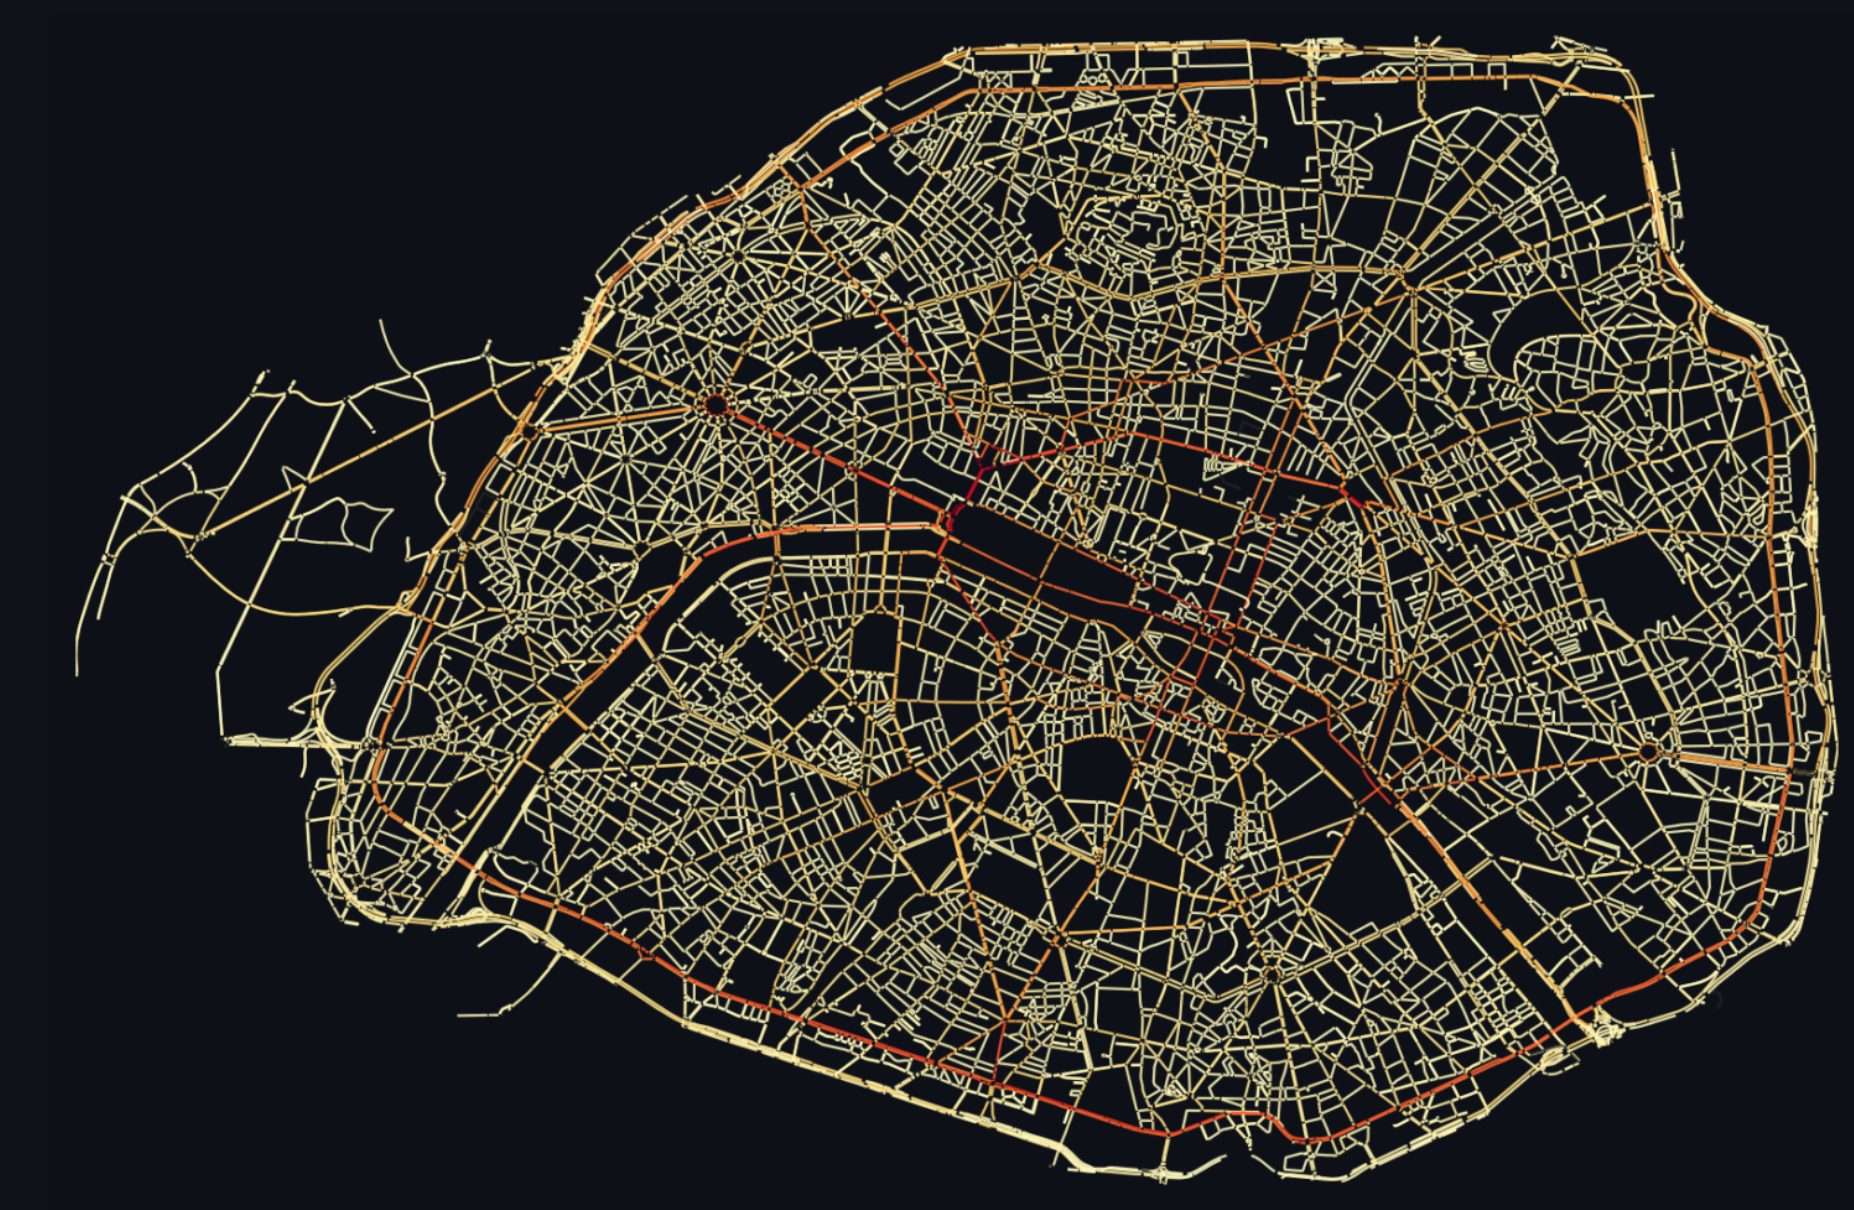
\includegraphics[keepaspectratio,alt={Visualisations SIG colorées du réseau routier après une simulation de pointe de 1 heure. Les segments routiers sont colorés du gris (fluide) au rouge (saturation complète / gridlock)}]{images/paris-heat_map_trafic.png}}
\pandocbounded{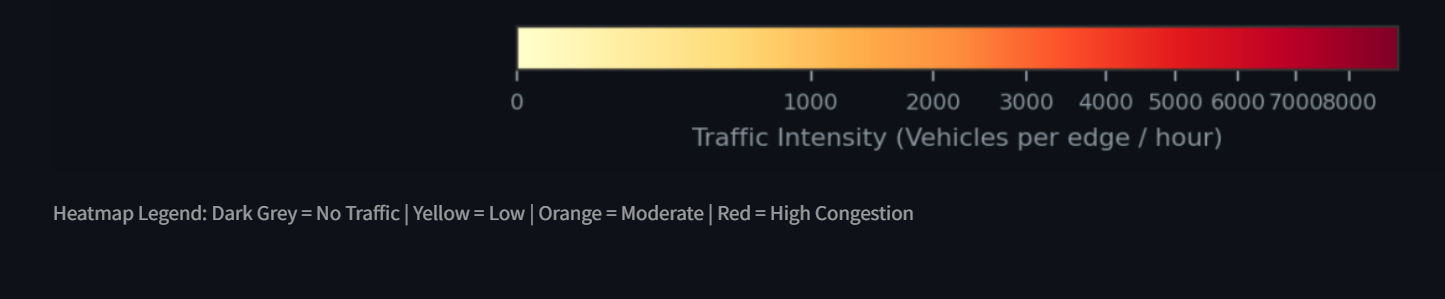
\includegraphics[keepaspectratio,alt={Visualisations SIG colorées du réseau routier après une simulation de pointe de 1 heure. Les segments routiers sont colorés du gris (fluide) au rouge (saturation complète / gridlock)}]{images/paris-heat_map-legend.png}}

\subsubsection{Section 3 : Perspectives
opérationnelles}\label{section-3-perspectives-opuxe9rationnelles}

La complémentarité des deux approches développées dans ce mémoire ouvre
la voie à un cadre d'optimisation urbaine hybride (IA-SUMO) alliant la
rapidité de l'apprentissage machine et la précision de la simulation
physique. Dans ce schéma opérationnel, le modèle prédictif basé sur l'IA
(XGBoost) est utilisé en amont pour explorer rapidement de larges
espaces de solutions (par exemple, tester des milliers d'implantations
géométriques de voirie ou de localisations de hubs de recharge). L'IA
évalue chaque configuration en une fraction de seconde, éliminant les
scénarios inefficaces et sélectionnant les configurations optimales. Les
scénarios retenus par le modèle prédictif sont ensuite injectés dans le
jumeau numérique microscopique haute-fidélité (SUMO) pour affiner
l'analyse locale (vérification des files d'attente au mètre près,
comportement d'évitement des deux-roues, impact électrique précis).

Les résultats de ce travail de recherche font d'ailleurs l'objet d'une
valorisation académique à travers la préparation de deux publications
scientifiques de fin d'année. La première publication, co-écrite avec
VinUniversity, s'intitule \emph{``Microscopic Traffic Flow and Emission
Modeling of High-Power Electric Vehicle Charging Infrastructure in
Hyper-Dense Master-Planned Communities: The Case of Sao Bien, Vinhomes
Ocean Park.''} (présentation du protocole YOLOv8, de l'architecture du
jumeau numérique SUMO et de l'évaluation des scénarios de
densification). La deuxième publication s'intitule \emph{``Topological
Graph-Spectral Machine Learning for Real-Time Urban CO2 Emissions
Prediction: Applying Kato's Perturbation Theory and Kreiss Constants to
Non-Normal Urban Networks.''} (formalisation de la méthode de prédiction
spectrale sur graphes non-symétriques, étude de la stabilité via la
constante de Kreiss et performances de XGBoost).

\newpage

\section{CONCLUSION}\label{conclusion}

Ce travail de recherche a permis de jeter les bases d'un double cadre
méthodologique pour la modélisation de la mobilité urbaine décarbonée.
Nos travaux s'articulent ainsi autour d'un double objectif de recherche
complémentaire.

D'une part, nous avons développé des jumeaux numériques microscopiques
de haute-fidélité capables de modéliser l'impact cinématique local de
l'intégration d'infrastructures de recharge pour véhicules électriques.
Ce travail a été appliqué sur le quartier résidentiel à haute densité de
Sao Bien à Hanoï. Il a permis d'intégrer des comportements stochastiques
de charge et de documenter des dynamiques de trafic spécifiques comme
l'inversion modale de vacances (\emph{Holiday Reversal}), le tout
calibré par des données réelles issues de notre protocole de vision par
ordinateur YOLOv8.

D'autre part, nous avons proposé une méthode de rupture basée sur
l'intelligence artificielle topologique spectrale. En exploitant la
structure mathématique de la matrice d'adjacence du réseau urbain (rayon
spectral, constante de Kreiss, perturbations de Kato) et l'algorithme
XGBoost, nous avons démontré qu'il est possible d'estimer instantanément
la pollution d'une ville sans simuler individuellement chaque véhicule,
contournant ainsi les limites computationnelles traditionnelles (RAM,
SWAP) à l'échelle macroscopique.

La boucle d'optimisation hybride (IA-SUMO) constitue la perspective
ultime de ces travaux, permettant d'optimiser l'aménagement urbain à
grande échelle tout en conservant une précision physique sur les points
sensibles du réseau. Enfin, la valorisation académique de ces recherches
à travers la rédaction de deux articles scientifiques de fin d'année
témoigne de la rigueur et de la portée de la méthodologie développée.

\newpage

\section{BIBLIOGRAPHIE SCIENTIFIQUE ET
ACADÉMIQUE}\label{bibliographie-scientifique-et-acaduxe9mique}

\begin{itemize}
\tightlist
\item
  Agarwal, M., Maze, T. H., \& Souleyrette, R. (2005). \emph{Impacts of
  Weather on Urban Freeway Traffic Flow Characteristics and Facility
  Capacity}. Center for Transportation Research and Education, Iowa
  State University.
\item
  Boeing, G. (2017). \emph{OSMnx: New methods for acquiring,
  constructing, analyzing, and visualizing complex street networks}.
  Computers, Environment and Urban Systems, 65, 126-139.
\item
  Braess, D. (1968). \emph{Über ein Paradoxon aus der Verkehrsplanung}.
  Unternehmensforschung, 12, 258-268.
\item
  Easley, D., \& Kleinberg, J. (2010). \emph{Networks, Crowds, and
  Markets: Reasoning about a Highly Connected World}. Cambridge
  University Press.
\item
  Forrester, J. W. (1969). \emph{Urban Dynamics}. Productivity Press.
\item
  Kato, T. (1995). \emph{Perturbation Theory for Linear Operators} (Vol.
  132). Springer Science \& Business Media.
\item
  Krajzewicz, D., Erdmann, J., Behrisch, M., \& Bieker, L. (2012).
  \emph{Recent development and applications of SUMO - Simulation of
  Urban MObility}. International Journal on Advances in Systems and
  Measurements, 5(3\&4), 128-138.
\item
  Kratzsch, V. et al.~(2020). \emph{HBEFA Version 4.1 -- Handbook
  Emission Factors for Road Transport}. INFRAS.
\item
  Kreiss, H. O. (1962). \emph{Über die Stabilitätsdefinition für
  Differenzengleichungen, die partielle Differentialgleichungen
  approximieren}. BIT Numerical Mathematics, 2(3), 153-181.
\item
  Mitchell, M. (2009). \emph{Complexity: A Guided Tour}. Oxford
  University Press.
\item
  Thocle (2025). \emph{Realistic Urban Traffic Generator using
  Decentralized Federated Learning for the SUMO simulator}.
  arXiv:2506.07980.
\item
  Trefethen, L. N., \& Embree, M. (2005). \emph{Spectra and
  Pseudospectra: The Behavior of Nonnormal Matrices and Operators}.
  Princeton University Press.
\end{itemize}

\newpage

\section{RÉFÉRENCES WEB ET INSTITUTIONNELLES
(WEBOGRAPHIE)}\label{ruxe9fuxe9rences-web-et-institutionnelles-webographie}

\begin{itemize}
\tightlist
\item
  Aimsun (2024). \emph{Aimsun Next User Manual}. Aimsun SLU.
  \url{https://www.aimsun.com/}
\item
  Apur (2025). \emph{Évolution des mobilités et du parc automobile dans
  la Métropole du Grand Paris au 1er Janvier 2025}. Atelier Parisien
  d'Urbanisme.
\item
  Avere-France (2025). \emph{Baromètre national des infrastructures de
  recharge de véhicules électriques}.
  \url{https://www.avere-france.org/}
\item
  City of Paris (2024). \emph{Rapport d'activité sur les déplacements et
  la circulation à Paris en 2023}. Mairie de Paris.
\item
  European Environment Agency (EEA) (2024). \emph{Transport and
  Mobility: Transitioning to Sustainable Systems}. EEA Report.
  \url{https://www.eea.europa.eu/}
\item
  French Government (2026). \emph{Bonus écologique et primes pour
  l'acquisition d'un véhicule électrique}. Service-Public.fr.
  \url{https://www.service-public.fr/}
\item
  Green SM (2025). \emph{GSM: Green and Smart Mobility electric fleet
  expansion}. GSM Joint Stock Company. \url{https://www.green-sm.com/}
\item
  International Energy Agency (IEA) (2025). \emph{Road Transport --
  Breakthrough Agenda Report 2025}. IEA. \url{https://www.iea.org/}
\item
  MATsim (2024). \emph{Multi-Agent Transport Simulation (MATSim)
  Documentation}. MATsim Community. \url{https://www.matsim.org/}
\item
  OECD (2024). \emph{Urban Mobility and Decarbonisation}. Organisation
  for Economic Co-operation and Development. \url{https://www.oecd.org/}
\item
  PTV Group (2024). \emph{PTV Vissim User Manual: Microscopic Traffic
  Flow Simulation}. \url{https://www.ptvgroup.com/}
\item
  Streamlit Inc.~(2020). \emph{Streamlit: The fastest way to build and
  share data applications for machine learning}.
  \url{https://streamlit.io/}
\item
  SUMO (2024). \emph{SUMO User Documentation}. German Aerospace Center
  (DLR). \url{https://sumo.dlr.de/}
\item
  Texas A\&M Transportation Institute (2021). \emph{Urban Mobility
  Report}. Texas A\&M University. \url{https://mobility.tamu.edu/}
\item
  United Nations, Department of Economic and Social Affairs (2018).
  \emph{World Urbanization Prospects: The 2018 Revision}. United
  Nations. \url{https://www.un.org/}
\item
  United Nations, Department of Economic and Social Affairs (2018).
  \emph{Sustainable Urbanization is Key to Successful Development}.
  United Nations. \url{https://www.un.org/}
\item
  VinBus (2021). \emph{VinBus officially operates the first smart
  electric bus in Vietnam}. VinBus Ecology Transport Services.
  \url{https://vinbus.vn/}
\item
  Vinhomes (2024). \emph{Vinhomes Ocean Park: Urban Development and
  Master-Planned Communities}. Vinhomes Joint Stock Company.
  \url{https://oceanpark.vinhomes.vn/}
\item
  World Bank (2024). \emph{Urban Development Overview}. World Bank
  Group. \url{https://www.worldbank.org/}
\end{itemize}

\newpage

\section{ANNEXES : TABLEAUX COMPLÉMENTAIRES DES RUNS DE SIMULATION
MULTI-VILLES}\label{annexes-tableaux-compluxe9mentaires-des-runs-de-simulation-multi-villes}

\subsubsection{Tableau 7 : Extrait des indicateurs macroscopiques des
simulations de
référence}\label{tableau-7-extrait-des-indicateurs-macroscopiques-des-simulations-de-ruxe9fuxe9rence}

{\def\LTcaptype{none} % do not increment counter
\begin{longtable}[]{@{}
  >{\raggedright\arraybackslash}p{(\linewidth - 14\tabcolsep) * \real{0.1053}}
  >{\raggedright\arraybackslash}p{(\linewidth - 14\tabcolsep) * \real{0.1053}}
  >{\centering\arraybackslash}p{(\linewidth - 14\tabcolsep) * \real{0.1316}}
  >{\centering\arraybackslash}p{(\linewidth - 14\tabcolsep) * \real{0.1316}}
  >{\centering\arraybackslash}p{(\linewidth - 14\tabcolsep) * \real{0.1316}}
  >{\centering\arraybackslash}p{(\linewidth - 14\tabcolsep) * \real{0.1316}}
  >{\centering\arraybackslash}p{(\linewidth - 14\tabcolsep) * \real{0.1316}}
  >{\centering\arraybackslash}p{(\linewidth - 14\tabcolsep) * \real{0.1316}}@{}}
\toprule\noalign{}
\begin{minipage}[b]{\linewidth}\raggedright
Date \& Time
\end{minipage} & \begin{minipage}[b]{\linewidth}\raggedright
City
\end{minipage} & \begin{minipage}[b]{\linewidth}\centering
Vehicles
\end{minipage} & \begin{minipage}[b]{\linewidth}\centering
Avg Speed
\end{minipage} & \begin{minipage}[b]{\linewidth}\centering
CO₂ Emitted
\end{minipage} & \begin{minipage}[b]{\linewidth}\centering
Weather
\end{minipage} & \begin{minipage}[b]{\linewidth}\centering
EV Adoption
\end{minipage} & \begin{minipage}[b]{\linewidth}\centering
Execution Time
\end{minipage} \\
\midrule\noalign{}
\endhead
\bottomrule\noalign{}
\endlastfoot
2026-06-08 11:37:40 & \textbf{Sydney} & 47 239 & 2.76 km/h & 174.23 Tons
& Clear (Optimal) & 15\% & 2602.90 s \\
2026-06-08 10:15:27 & \textbf{Rio de Janeiro} & 64 172 & 2.72 km/h &
265.52 Tons & Clear (Optimal) & 15\% & 3787.60 s \\
2026-06-08 09:58:55 & \textbf{Monaco} & 6 080 & 5.86 km/h & 21.46 Tons &
Clear (Optimal) & 8\% & 185.89 s \\
2026-06-06 10:55:18 & \textbf{Casablanca} & 49 785 & 15.62 km/h & 172.64
Tons & Clear (Optimal) & 10\% & 17605.75 s \\
2026-06-06 09:30:40 & \textbf{London} & 68 239 & 1.52 km/h & 241.86 Tons
& Clear (Optimal) & 15\% & 4545.16 s \\
2026-05-22 11:31:03 & \textbf{Sydney} & 55 453 & 2.21 km/h & 215.45 Tons
& Clear (Optimal) & 15\% & 3752.45 s \\
2026-05-22 10:33:58 & \textbf{Chamonix} & 2 000 & 46.50 km/h & 2.32 Tons
& Clear (Optimal) & 8\% & 13.07 s \\
2026-05-21 11:54:12 & \textbf{Versailles} & 1 000 & 31.46 km/h & 0.76
Tons & Clear (Optimal) & 10\% & 18.96 s \\
2026-05-13 20:22:36 & \textbf{Versailles} & 20 450 & 2.31 km/h & 82.06
Tons & Clear (Optimal) & 10\% & 521.54 s \\
2026-05-12 15:36:46 & \textbf{Madrid} & 98 560 & 16.19 km/h & 352.83
Tons & Clear (Optimal) & 10\% & 12276.98 s \\
2026-05-12 11:03:53 & \textbf{Paris} & 128 644 & 3.08 km/h & 508.20 Tons
& Clear (Optimal) & 10\% & 5971.15 s \\
2026-04-13 06:07:41 & \textbf{Paris} & 92 173 & 4.75 km/h & 338.01 Tons
& Clear (Optimal) & 10\% & 4126.56 s \\
2026-04-12 12:14:49 & \textbf{Paris} & 90 909 & 4.06 km/h & 341.46 Tons
& Clear (Optimal) & 10\% & 4340.81 s \\
2026-04-12 08:06:36 & \textbf{Paris} & 48 554 & 8.74 km/h & 152.21 Tons
& Clear (Optimal) & N/A & 2036.43 s \\
2026-04-11 16:47:14 & \textbf{Paris} & 48 641 & 7.93 km/h & 151.69 Tons
& Clear (Optimal) & N/A & 2051.00 s \\
2026-04-11 16:11:53 & \textbf{Versailles} & 12 750 & 4.26 km/h & 49.45
Tons & Clear (Optimal) & N/A & 219.36 s \\
2026-04-11 13:25:05 & \textbf{Paris} & 48 669 & 9.09 km/h & 166.46 Tons
& Clear (Optimal) & N/A & 2039.20 s \\
\end{longtable}
}

\subsubsection{\texorpdfstring{Tableau 8 : Répartition des tonnages de
\(CO_2\) émis par classe de véhicule de la
flotte}{Tableau 8 : Répartition des tonnages de CO\_2 émis par classe de véhicule de la flotte}}\label{tableau-8-ruxe9partition-des-tonnages-de-co_2-uxe9mis-par-classe-de-vuxe9hicule-de-la-flotte}

{\def\LTcaptype{none} % do not increment counter
\begin{longtable}[]{@{}
  >{\raggedright\arraybackslash}p{(\linewidth - 12\tabcolsep) * \real{0.1212}}
  >{\raggedright\arraybackslash}p{(\linewidth - 12\tabcolsep) * \real{0.1212}}
  >{\centering\arraybackslash}p{(\linewidth - 12\tabcolsep) * \real{0.1515}}
  >{\centering\arraybackslash}p{(\linewidth - 12\tabcolsep) * \real{0.1515}}
  >{\centering\arraybackslash}p{(\linewidth - 12\tabcolsep) * \real{0.1515}}
  >{\centering\arraybackslash}p{(\linewidth - 12\tabcolsep) * \real{0.1515}}
  >{\centering\arraybackslash}p{(\linewidth - 12\tabcolsep) * \real{0.1515}}@{}}
\toprule\noalign{}
\begin{minipage}[b]{\linewidth}\raggedright
Date \& Time
\end{minipage} & \begin{minipage}[b]{\linewidth}\raggedright
City
\end{minipage} & \begin{minipage}[b]{\linewidth}\centering
Total CO₂
\end{minipage} & \begin{minipage}[b]{\linewidth}\centering
Cars CO₂
\end{minipage} & \begin{minipage}[b]{\linewidth}\centering
Motorcycles CO₂
\end{minipage} & \begin{minipage}[b]{\linewidth}\centering
Buses CO₂
\end{minipage} & \begin{minipage}[b]{\linewidth}\centering
Trucks CO₂
\end{minipage} \\
\midrule\noalign{}
\endhead
\bottomrule\noalign{}
\endlastfoot
2026-06-08 11:37:40 & \textbf{Sydney} & \textbf{174.23 T} & 88.43 T &
37.37 T & 23.26 T & 25.18 T \\
2026-06-08 10:15:27 & \textbf{Rio de Janeiro} & \textbf{265.52 T} &
134.77 T & 56.41 T & 36.30 T & 38.04 T \\
2026-06-08 09:58:55 & \textbf{Monaco} & \textbf{21.46 T} & 17.24 T &
2.26 T & 0.95 T & 1.01 T \\
2026-06-06 10:55:18 & \textbf{Casablanca} & \textbf{172.64 T} & 104.59 T
& 26.36 T & 24.60 T & 17.09 T \\
2026-06-06 09:30:40 & \textbf{London} & \textbf{241.86 T} & 123.13 T &
53.54 T & 31.05 T & 34.14 T \\
2026-05-22 11:31:03 & \textbf{Sydney} & \textbf{215.45 T} & 109.64 T &
46.80 T & 28.13 T & 30.89 T \\
2026-05-22 10:33:58 & \textbf{Chamonix} & \textbf{2.32 T} & 1.88 T &
0.23 T & 0.11 T & 0.10 T \\
2026-05-21 11:54:12 & \textbf{Versailles} & \textbf{0.76 T} & 0.54 T &
0.12 T & 0.08 T & 0.03 T \\
2026-05-13 20:22:36 & \textbf{Versailles} & \textbf{82.06 T} & 57.07 T &
14.03 T & 7.12 T & 3.83 T \\
2026-05-12 15:36:46 & \textbf{Madrid} & \textbf{352.83 T} & 178.47 T &
79.62 T & 55.68 T & 39.05 T \\
2026-05-12 11:03:53 & \textbf{Paris} & \textbf{508.20 T} & 374.95 T &
105.01 T & 9.15 T & 19.10 T \\
2026-04-13 06:07:41 & \textbf{Paris} & \textbf{338.01 T} & 270.84 T &
47.96 T & 6.28 T & 12.93 T \\
2026-04-12 12:14:49 & \textbf{Paris} & \textbf{341.46 T} & 155.06 T &
88.45 T & 63.24 T & 34.71 T \\
2026-04-12 08:06:36 & \textbf{Paris} & \textbf{152.21 T} & 69.28 T &
38.10 T & 29.29 T & 15.53 T \\
2026-04-11 16:47:14 & \textbf{Paris} & \textbf{151.69 T} & 68.97 T &
38.21 T & 29.13 T & 15.38 T \\
2026-04-11 16:11:53 & \textbf{Versailles} & \textbf{49.45 T} & 0.00 T &
0.00 T & 0.00 T & 0.00 T \\
2026-04-11 13:25:05 & \textbf{Paris} & \textbf{166.46 T} & 0.00 T & 0.00
T & 0.00 T & 0.00 T \\
\end{longtable}
}

\subsubsection{Tableau 9 : Profil de performance informatique détaillé
(secondes
CPU)}\label{tableau-9-profil-de-performance-informatique-duxe9tailluxe9-secondes-cpu}

{\def\LTcaptype{none} % do not increment counter
\begin{longtable}[]{@{}
  >{\raggedright\arraybackslash}p{(\linewidth - 10\tabcolsep) * \real{0.1429}}
  >{\raggedright\arraybackslash}p{(\linewidth - 10\tabcolsep) * \real{0.1429}}
  >{\centering\arraybackslash}p{(\linewidth - 10\tabcolsep) * \real{0.1786}}
  >{\centering\arraybackslash}p{(\linewidth - 10\tabcolsep) * \real{0.1786}}
  >{\centering\arraybackslash}p{(\linewidth - 10\tabcolsep) * \real{0.1786}}
  >{\centering\arraybackslash}p{(\linewidth - 10\tabcolsep) * \real{0.1786}}@{}}
\toprule\noalign{}
\begin{minipage}[b]{\linewidth}\raggedright
Date \& Time
\end{minipage} & \begin{minipage}[b]{\linewidth}\raggedright
City
\end{minipage} & \begin{minipage}[b]{\linewidth}\centering
Dijkstra Routing
\end{minipage} & \begin{minipage}[b]{\linewidth}\centering
SUMO Physics Engine
\end{minipage} & \begin{minipage}[b]{\linewidth}\centering
XML Parsing
\end{minipage} & \begin{minipage}[b]{\linewidth}\centering
Total Duration
\end{minipage} \\
\midrule\noalign{}
\endhead
\bottomrule\noalign{}
\endlastfoot
2026-06-08 11:37:40 & \textbf{Sydney} & 666.64 s & 1934.63 s & 1.58 s &
\textbf{2602.90 s} \\
2026-06-08 10:15:27 & \textbf{Rio de Janeiro} & 555.46 s & 3229.83 s &
2.30 s & \textbf{3787.60 s} \\
2026-06-08 09:58:55 & \textbf{Monaco} & 7.69 s & 178.03 s & 0.16 s &
\textbf{185.89 s} \\
2026-06-06 10:55:18 & \textbf{Casablanca} & 13577.62 s & 4026.18 s &
1.89 s & \textbf{17605.75 s} \\
2026-06-06 09:30:40 & \textbf{London} & 1886.52 s & 2655.74 s & 2.90 s &
\textbf{4545.16 s} \\
2026-05-22 11:31:03 & \textbf{Sydney} & 997.87 s & 2752.49 s & 2.08 s &
\textbf{3752.45 s} \\
2026-05-22 10:33:58 & \textbf{Chamonix} & 4.27 s & 8.75 s & 0.04 s &
\textbf{13.07 s} \\
2026-05-21 11:54:12 & \textbf{Versailles} & 6.07 s & 12.84 s & 0.03 s &
\textbf{18.96 s} \\
2026-05-13 20:22:36 & \textbf{Versailles} & 48.35 s & 472.63 s & 0.55 s
& \textbf{521.54 s} \\
2026-05-12 15:36:46 & \textbf{Madrid} & 9716.06 s & 2558.17 s & 2.72 s &
\textbf{12276.98 s} \\
2026-05-12 11:03:53 & \textbf{Paris} & 3371.01 s & 2596.00 s & 4.13 s &
\textbf{5971.15 s} \\
2026-04-13 06:07:41 & \textbf{Paris} & 2353.06 s & 1770.98 s & 2.50 s &
\textbf{4126.56 s} \\
2026-04-12 12:14:49 & \textbf{Paris} & 2421.37 s & 1916.28 s & 3.16 s &
\textbf{4340.81 s} \\
2026-04-12 08:06:36 & \textbf{Paris} & 1167.02 s & 868.03 s & 1.37 s &
\textbf{2036.43 s} \\
2026-04-11 16:47:14 & \textbf{Paris} & 1134.40 s & 915.39 s & 1.20 s &
\textbf{2051.00 s} \\
2026-04-11 16:11:53 & \textbf{Versailles} & 17.36 s & 201.73 s & 0.26 s
& \textbf{219.36 s} \\
2026-04-11 13:25:05 & \textbf{Paris} & 1145.37 s & 892.65 s & 1.17 s &
\textbf{2039.20 s} \\
\end{longtable}
}

\end{document}
